\chapter{Equip Expectation Maximization with Normalizing Flows}
\label{chpt6:em-flow}
\graphicspath{{source/chapter6/}}

When learning with partially observed variables in graphical models, EM is one of the most widely used frameworks in practices. In directed graphical models, immediate relief is that we do not need to deal with the partition function $Z(\bm{\theta})$ anymore. However, it does not mean directed graphical models with partially observed variables are trivial to learn. The 'missing' data (corresponding to unobserved variables) still poses challenges in model learning, since we want to have the partial evidence (observed) well explained by our model while keeping its ability to track uncertainty of the 'unobserved' part.

As discussed in section~\ref{chpt2:sec:learning-principles}, the presence of latent or hidden variables is either due to the data availability or abstraction of data generating. Once the dataset is given, the option left to us is the choice of the model that we plan to use to approximate the true distribution $p^{\ast}$ which actually generated the dataset. This process is to select one model from a set of models, i.e. hypothesis space, based on the likelihood criteria. If the hypothesis space is very limited, the ability to represent our true $p^{\ast}$ is limited, leading to the inherent error. This type of inherent limitation brings learning \textit{bias} before we start to fit the parameters.
Therefore, given that the dataset is large and representative enough, we hope that the hypothesis space is highly expressive such that we are more likely to be able to represent $p^{\ast}$ with a selected model from the hypothesis space. This naturally requires our model to be flexible and expressive.

Gaussian mixture model has been successfully applied widely with EM framework, which also enjoys the closed-form update rule in iterations. The advantage comes with the limitation of linear dependency and free parameters that can be tuned, i.e. limitation of flexibility. To explore further, we discuss more flexible models beyond Gaussian in this chapter. We start by inducing the normalizing flows that are going to be used as probabilistic models in place of Gaussian models. A normalizing flow can consist of as many non-linear transformations as needed, and thus is highly flexible. Besides, likelihood computation ability remains and it allows efficient sampling in normalizing flow. But closed-form iterative update solutions are not available anymore. We, therefore, need to design the practical algorithms to model learning in EM framework.


\section{Normalizing Flow}
Normalizing flow is a practical approach to improve the flexibility of probabilistic models while still keeping the likelihood computation tractable and the efficiency of generating samples. The general idea is to start with an initial random variable following a relatively simple distribution with known probability density function. Then a chain of invertible parameterized transformations is applied to the initial random variable such that the output follows a more flexible distribution.

Denote the chain of transformations by $\tilde{\bm{g}}$ and the output by $\tilde{\bm{x}}\in \RR^{N}$. Then we have
\begin{equation}
  \tilde{\bm{x}}=\tilde{\bm{g}}(\bm{z})
\end{equation}
where $\bm{z}\in \RR^{N}$ is the initial random variable with know density function $p(\bm{z})$. To explicitly denote the chain,
\begin{equation}
  \tilde{\bm{g}}=\tilde{\bm{g}}^{[L]}\circ \tilde{\bm{g}}^{[L-1]}\circ \cdots
  \circ \tilde{\bm{g}}^{[1]},
\end{equation}
which is invertible $\tilde{\bm{f}}=\tilde{\bm{g}}^{-1}$. Then the signal flow can be depicted as% , illustrated in \autoref{illustation}.
\begin{equation*}
  \centering
  \begin{tikzpicture}
    \node (z) at (0,0) {};
    \node at ($(z)-(0.5,0)$){$\bm{z}=\bm{h}_0$};
    \node (xi1) at (1.5,0) {$\bm{h}_1$};
    \node (xi2) at (3,0) {};
    \node (xi3) at (4.5,0){};
    \node (x) at (6,0) {};
    \node at ($(x)+(0.5,0)$){$\tilde{\bm{x}} = \bm{h}_L$};
    \draw[->] ($(z) + (0.3,0.1)$) -- node[above]{$\tilde{\bm{g}}^{[1]}$} ($(xi1)+(-0.3,0.1)$); 
    \draw[->] ($(xi1)-(0.3,0.1)$) -- node[below]{$\tilde{\bm{f}}^{[1]}$}($(z) - (-0.3,0.1)$);
    \draw[->] ($(xi1) + (0.3,0.1)$) -- node[above]{$\tilde{\bm{g}}^{[2]}$} ($(xi2)+(-0.3,0.1)$); 
    \draw[->] ($(xi2)-(0.3,0.1)$) -- node[below]{$\tilde{\bm{f}}^{[2]}$}($(xi1) - (-0.3,0.1)$);
    \draw[->] ($(xi3) + (0.3,0.1)$) -- node[above]{$\tilde{\bm{g}}^{[L]}$} ($(x)+(-0.3,0.1)$); 
    \draw[->] ($(x)-(0.3,0.1)$) -- node[below]{$\tilde{\bm{f}}^{[L]}$}($(xi3) - (-0.3,0.1)$);
    \draw[dotted,line width = 0.3 mm] (xi2) -- (xi3);
  \end{tikzpicture}
\end{equation*}
where $\tilde{\bm{g}}^{[l]}$ and $\tilde{\bm{f}}^{[l]}$ are the $l$-th transformation in $\tilde{\bm{g}}$ and $\tilde{\bm{f}}$, respectively. In practice, $\bm{\tilde}{g}$ can be implemented by feed-forward neural networks, which we will detail later.

If every transformation in the chain of the flow is invertible, the full mapping is invertible.
Then, the probability density function relation between $p(\bm{z})$ and $p(\tilde{\bm{x}})$ follows the change of variable formula
\begin{equation}\label{chpt6:eq:change-var}
  p(\tilde{\bm{x}}) =  p(\bm{z}) \bigg| \mathrm{det}(\bm{J}) \big|_{\bm{z}=\tilde{\bm{f}}(\tilde{\bm{x}})}\bigg|,
\end{equation}
where $\mathrm{det}(\bm{J})$ denotes the determinant of Jacobian $\bm{J}$
\begin{equation}
  \bm{J} = \left[
    \begin{array}{ccc}
      \frac{\partial \tilde{f}_1}{\partial \tilde{x}_1} & \hdots & \frac{\partial \tilde{f}_1}{\partial \tilde{x}_N} \\
      \vdots & \hdots & \vdots \\
      \frac{\partial \tilde{f}_N}{\partial \tilde{x}_1} & \hdots & \frac{\partial \tilde{f}_N}{\partial \tilde{x}_N}
    \end{array}
  \right].
\end{equation}
The challenge lies at the determinant computation of Jacobian $\bm{J}$, or equivalently that of each transformation $\tilde{\bm{g}}^{[l]}$. \cite{DBLP:journals/corr/DinhKB14} introduced the model NICE to transform only half of the variables at a chain step, which results in triangular Jacobian of the transformation. If each transformation has a triangular Jacobian, determinant computation would be efficient in \eqref{chpt6:eq:change-var}.
This flow architecture divides the feature $\bm{h}_l$ at the $l$'th layer into two subparts as
$\bm{h}_l = [\bm{h}_{l,a}^{\intercal} \, , \, \bm{h}_{l,b}^{\intercal}]^{\intercal}$ where
$(\cdot)^{\intercal}$ denotes transpose operation. Then considering $\bm{h}_0 = \bm{z}$, we have the following forward and inverse relations between $(l-1)$'th and $l$'th layers:
\begin{equation}\label{eq-gl}
  \begin{array}{l}
    \bm{h}_{l-1} =
    \begin{bmatrix}
      \bm{h}_{l-1,a}\\
      \bm{h}_{l-1,b}
    \end{bmatrix}
    =
    \begin{bmatrix}
      \bm{h}_{l,a}\\
      \bm{m}_a(\bm{h}_{l,a})\odot \bm{h}_{l,b} + \bm{m}_b(\bm{h}_{l,a})
    \end{bmatrix},\vspace{10pt}\\
    \bm{h}_{l} =
    \begin{bmatrix}
      \bm{h}_{l,a}\\
      \bm{h}_{l,b}
    \end{bmatrix}
    =
    \begin{bmatrix}
      \bm{h}_{l-1,a}\\
      \left(  \bm{h}_{l-1,b} - \bm{m}_b(\bm{h}_{l-1,a}) \right)\oslash \bm{m}_a(\bm{h}_{l-1,a}) 
    \end{bmatrix}, \\
  \end{array}  
\end{equation}
where $\odot$ denotes element-wise product, $\oslash$ denotes
element-wise division, and $\bm{m}_a(\cdot), \bm{m}_b(\cdot)$ can be
complex non-linear mappings (implemented by neural networks).
For the flow model, the determinant of Jacobian matrix is
\begin{equation}
  \begin{array}{rl}
    \mathrm{det}(\bm{J}) |_{\bm{z}=\tilde{\bm{f}}(\tilde{\bm{x}})} & = \prod_{l=1}^L \det (\bm{J}_l) |_{\bm{h}_{l}},
  \end{array}
\end{equation}
where $\bm{J}_l$ is the Jacobian of the transformation from the $l$-th layer to the $(l-1)$-th layer, i.e., the inverse transformation. We compute the determinate of the Jacobian matrix as
\begin{align}\label{eq-hl-determinate}
  \det (\bm{J}_l)|_{\bm{h}_{l}}& = \det \left[  \pd{\bm{h}_{l-1}}{\bm{h}_l} \right] \nonumber\\
                               & = \det
                                 \begin{bmatrix}
                                   \bm{I}_a & \mathbf{0} \nonumber\\
                                   \pd{\bm{h}_{l-1,b}}{\bm{h}_{l,a}} & \mathrm{diag}(\bm{m}_a(\bm{h}_{l,a}))
                                 \end{bmatrix}\nonumber\\
                               &= \det \left( \mathrm{diag}(\bm{m}_a(\bm{h}_{l,a})) \right),
\end{align}
where $\bm{I}_a$ is identity matrix and $\mathrm{diag}(\cdot)$ returns a square matrix with the elements of $(\cdot)$ on the main diagnal. Then the pdf is
\begin{align}
  p(\tilde{\bm{x}}) & =  p(\bm{z}) \big| \mathrm{det}(\bm{J}) |_{\bm{z}=\tilde{\bm{f}}(\tilde{\bm{x}})}\big| \nonumber\\
                    &  = p(\bm{z}) \prod_{l=1}^L \abs{\det\left( \mathrm{diag}(\bm{m}_a(\bm{h}_{l,a}))]  \right)}.
\end{align}
\eqref{eq-gl} describes a \textit{coupling} mapping between layers. Since the coupling has a partial identity mapping, direct concatenation of multiple such coupling mappings would result in a partial identity mapping of the overall mapping $\tilde{\bm{g}}$. Therefore, techniques such as alternating the positions of identity mapping \cite{2016arXiv160508803D} or using $1\times1$ convolution operations \cite{2018arXiv180703039K} before each coupling mapping are used to treat the issue.
Sometimes, it may not be necessary to carry all features thorough all $L$ chain steps. For instance, \cite{2016arXiv160508803D}\cite{2018arXiv180703039K} split some hidden
layer signal $\bm{h}$ and model a part of it directly as standard Gaussian to reduce computation and memory burden.

\begin{remark}
  There are alternative ways of formulating the transformation of variable changing while maintaining efficient computation of the Jacobian determinant. Inverse autoregreeesive flow (IAF) was proposed in \cite{rezende2015variational}. In the IAF model, a chain step of transformation is
  \begin{equation*}
    \bm{h}_l = \bm{h}_{l-1} + \bm{u} \cdot {m}(\bm{w}^{\intercal} \cdot \bm{h}_{l-1} + b)
  \end{equation*}
  where $m$ is non-linear mapping, $\bm{w}, \bm{u}~\in \RR^{N}$ and $b\in \RR$. IAF does no use partial identity mapping as NICE. Its Jacobian is not triangular and thus determinant computation is more expensive. The followed work by \cite{kingma2016IVF} created element-wise transformation in a customized way to improve IAF such the Jacobian becomes a triangular matrix. 
  
  In contrast to the above finite-chain flow where $L$ is a discrete finite integer, the method developed in \cite{ricky2018ODE} introduced a continuous-transformation of variables by solving an ordinary differential equation (ODE). Comparing to the discrete finite chain of transformation in normalizing flow, ODE can be viewed as a continuous chain of variable transformation. The inverse mapping and Jacobian determinant are not required in ODE method. But ODE needs to solve differentiation equations which is also challenging.
\end{remark}



\section{expectation maximization of neural network based mixture models}

\section{An alternative construction method}

\section{Experiments}


\section{Summary}

\section{Raw material}
\section{Introduction}

% Recently a significant attention has been given to
The paradigm of neural network based implicit distribution
modeling has received a significant attention. In this paradigm, a neural network being a powerful non-linear function acts as an efficient generator. Prominent examples of neural network based implicit distributions are generative adversarial networks (GANs) \cite{NIPS2014_5423} and its
variants \cite{NIPS2016_6125,
  2018arXiv180508318Z, salimans2018improving}. GANs are efficient for generating samples and successful in several applications \cite{ledig2017photo}, \cite{NIPS2016_6125}. For a GAN, a latent variable is used as
an input to the generator neural network of the GAN and the output of the
neural network is considered to be a data sample from the implicit
distribution.  In implicit distribution modeling by GANs, neither
analytical form of the distribution nor likelihood for a data sample
is available. Naturally the use of neural network based implicit distribution models like GANs is restricted to many applications where it is important to compute likelihood, for example, maximum likelihood based classification.

% Naturally, this is a limitation to explore use of EM for design of neural network based implicit mixture models. %On the other hand, to the best of authors' knowledge, we are not aware of works on exploring EM for neural network based explicit mixture models.

In this article, we focus on neural network based explicit distribution modeling. An explicit distribution model has an analytical functional form and we are able to compute likelihood. While use of neural network based generators in GANs for distribution modeling is powerful, we look for further improvements. In this regard, a standard practice is to use mixture models assuming that the underlying distribution is multi-modal, or data are spread over multiple manifolds and subspaces. Therefore we propose to design neural network based explicit mixture models such that they
\begin{enumerate}[noitemsep, nolistsep]
\item[(a)] have analytical forms, 
\item[(b)] offer the advantage of computing likelihood, and 
\item[(c)] retain the advantage of generating samples efficiently.
\end{enumerate}
With the advantage of computing likelihood, our proposed neural network based mixture models are suitable for maximum likelihood based classification. 

An important question is how to design practical algorithms to learn parameters of the proposed mixture models. In literature, expectation-maximization (EM) \cite{dempster1977maximum} is a standard approach for learning parameters of an explicit mixture model in a maximum likelihood framework, such as learning parameters of a Gaussian mixture model (GMM) \cite{Bishop:2006:PRM:1162264}. For realizing EM, computation of the
posterior distribution of a hidden variable (related to identity of a mixture component) given the observation
(visible signal/data) is required in the expectation step
(E-step). In addition, it is required to compute the joint log-likelihood of the observation signal and the hidden variable in the maximization step (M-step). For example, EM for GMM can be realized due to fullfilment of the above two requirements. Typically it is challenging to fulfill these two requirements for many other mixture distribution models. We also face the challenge to realize EM for learning parameters of neural network based explicit mixture models. This is due to the fact that use of neural networks in design of a system/algorithm/method often leads to loss of required level of analytical tractability. 

% We also face the challenge to realize EM for --->
% The challenge remains to releaze EM for ...

% It is often difficult to fulfill these two requirements for many  mixture distribution models due to analytical tractability. 
% For the case of learning GMM parameters, EM can be realized due to availability of computable likelihood and posterior. On the other hand, 
% It is a challenge to realize EM for learning parameters of neural network based explicit mixture models. Use of neural networks in a system often brings analytical complexities. 

In pursuit of neural network based explicit mixture models, our contributions in this article are as follows.
\begin{enumerate}[noitemsep, nolistsep]
\item[(a)] Proposing two mixture models - a high-complexity model and a low-complexity model. The low-complexity model uses shared parameters.
\item[(b)] Finding theoretical conditions for the models such that EM can be applied for their parameter learning. The theoretical conditions help to find explicit posterior and computation of expected likelihood. 
  % \item[(c)] \textcolor{blue}{Convergence analysis is provided for our proposed models and we provide a sufficient condition such that our models converge.}
\item[(c)] Designing practical algorithms for realization of EM where gradient search based optimization is efficiently embedded into M-step.
\item[(d)] Demonstrating efficiency of proposed mixture models through extensive experiments for generating samples and maximum likelihood based classification. 
\end{enumerate}
{At this point we mention the conditions of realizing EM to learn neural network based explicit mixture models.} The sufficient conditions are invertibility of associated neural networks and Jacobian computation of functional form of the neural networks. This helps to compute likelihood using change of variables. In practice we address the sufficient conditions using a flow-based neural network \cite{2018arXiv180703039K}.










% Learning of mixture distribution is a classic problem in
% pattern recognition and machine learning. Use of expectation maximization (EM)\cite{dempster1977maximum} is a standard approach for learning of mixture distribution model in a maximum likelihood framework, for example, learning a Gaussian mixture model (GMM) \cite{Bishop:2006:PRM:1162264}. Further extensions using variational inference for learning
% parameters of mixture models, such as GMM, beta mixture model have been explored in literature\cite{ma2011bayesian}.

% EM applies to explicit mixture distribution modeling. An explicit
% distribution has an analytical form and likelihood for
% a data sample can be computed. For realizing EM, computation of the
% posterior distribution of a latent variable given the observation
% (visible signal) is required firstly in the expectation step
% (E-step). In addition, it is required to compute the log-likelihood of joint observation signal and latent variable in the maximization step (M-step). It is often a challenge to fulfill these two requirements for many  mixture distribution models. 

% % For many models of practical interest, especially the
% % distribution models that are based on neural networks, it is
% % often infeasible to fulfill the above requirements of latent variable
% % posterior and joint logarithm likelihood computation.

% % Use of EM is traditionally explored for those mixture models where we
% % have computable analytical expressions for mixture distribution modeling. For example, GMM has an explicit analytical form and we can compute likelihood for a data point. %It is easy to 
% % calculate hidden variables (also known as responsibilities in EM literature) as posterior. 
% % GMM is comprised of a number of Gaussian components. We learn parameters of GMM which are the prior probabilities, mean vectors and covariance matrices for the Gaussian components. 

% % Analytical and computable expression of a mixture model helps for ease
% % of use. For example, we can easily calculate likelihood for a data sample, sampling from the distribution, etc. Further, learning of parameters of mixture model using machine learning approaches, such as EM may be realizable. 

% Recently machine learning community has given significant attention to
% the paradigm of neural network based implicit distribution
% modeling. In this paradigm, neural network based non-linear functions act as powerful generators. Prominent examples of neural network based implicit distributions are generative adversarial networks (GANs) \cite{NIPS2014_5423} and its
% variants \cite{NIPS2016_6125,
% 2018arXiv180508318Z, salimans2018improving}. GANs have shown
% success in several applications such as image super
% resolution \cite{ledig2017photo} and semi-supervised learning \cite{NIPS2016_6125}. A latent variable is used as
% an input to the generator neural network of GAN and the output of the
% neural network is considered to be a data sample from the implicit
% distribution. In implicit distribution modeling by GANs, neither
% analytical form of the distribution nor likelihood for a data sample
% is available. Naturally, this is a limitation to explore use of EM for design of neural network based implicit mixture models. %On the other hand, to the best of authors' knowledge, we are not aware of works on exploring EM for neural network based explicit mixture models.

% In this article, we explore use of EM for neural network based explicit mixture modeling. We propose two such mixture models that admit explicit, analytical expressions for the distributions and allow the computation of likelihood of data samples. We provide sufficient conditions to address the two requirements of EM in its E-step and M-step. The sufficient conditions are invertibility of associated neural networks and Jacobian computation of functional form of the neural networks. Therefore our main contribution in this article is to realize EM for neural network based explicit mixture models. We exploit power of EM for mixture modeling in maximum likelihood framework, as well as power of non-linear functional representation of neural networks. Our expectation is that the proposed mixture models are good for data with high diversity, where data distribution has multiple modes, or data are spread over multiple manifolds and subspaces.  


\subsection{Related Work and Background}
% \textcolor{blue}{We have to reduce size of this section. More compact writing necessary.}

% GANs do not provide explicit distribution models and they are
% trained by an adversary game, where neural network based generator and discriminator play against with each other to improve the implicit probability distribution induced by the generator. 
While GANs have high success in many applications, they are known to
suffer in a mode dropping problem where a generator of a GAN is unable
to capture all modes of an underlying probability distribution of data
\cite{2018arXiv180600880K}. To address diversity in data and model
multiple modes in a distribution, variants of generative models have been developed and
usage of multiple generators
has been considered. For instance, methods of minibatch discrimination \cite{NIPS2016_6125} and feature representation \cite{bang2018icml} are used to construct new discriminators of GANs which encourage the GANs to generate samples with diversity. Multiple Wasserstein GANs \cite{2017arXiv170107875A} are used in \cite{2018arXiv180600880K} with appropriate mutual information based regularization to encourage the diversity of samples generated by different GANs.
A mixture GAN approach is proposed in \cite{hoang2018mgan} using multiple generators and multi-classification solution to
encourage diversity of samples. Multi-agent diverse GAN \cite{DBLP:journals/corr/GhoshKNTD17} similarly employs $k$ generators, but uses a $(k+1)$-class discriminator instead of a typical binary discriminator to increase the diversity of generated samples. These works are implicit probability distribution modeling and thus prior distribution of generators can not be inferred when multiple generators are used.
% In all these existing GAN based mixture modeling method we do not have advantage of analytical form and computing prior distribution of generators. 

Typically, for a GAN, the latent variable is assumed to follow a known and fixed distribution, e.g., Gaussian. The latent signal for a given data sample can not be obtained since generators which are usually based on neural networks are non-invertible. The mapping from a data sample to its corresponding latent signal is approximately estimated by neural networks in different ways. \cite{donahue2017adversarial} and \cite{dumoulin2017adversarially} propose to train a
generative model and an inverse mapping (also neural network) from the data sample to the latent signal
simultaneously, using the adversarial training method of
GAN. Alternatively, \cite{dustin2017hierarchical}
proposes to approximately minimize a Kullback-Leibler divergence to
estimate the mapping from the data sample to the latent variable, which leads to a nontrivial probability density ratio estimation problem.

% \textcolor{blue}{Please compress this paragraph.}
Another track of
mixture modeling is based on ensembling method that combines weaker
learners together to boost the overall performance \cite{grover2017aaai_boost,
  2017arXiv170102386T}. In this approach mixture models are obtained as follows. Based on how well the current-step mixture model captures the underlying distribution, a new generative model is
trained to compensate the miss-captured part. However, measuring the difference between current-step mixture model and underlying distribution
of dataset quantitatively is a nontrivial task. In addition, since incremental building components are used in the mixture modeling, parallel training of model components is not feasible.


% is to combine weak or imperfect generative models to
% improve their overall performance, which is similar to boosting
% technique in supervised learning. In this type of approaches, an
% imperfect generative model is firstly trained directly using empirical dataset. Then the
% empirical dataset is reweighed to correct errors made by the trained imperfect
% generative model. Finally, a new generative model is trained on the reweighed
% empirical dataset. The reweighing step and new generative model
% training step are repeated, and these trained generative models are
% used in mixture way. \cite{grover2017aaai_boost} studies the application
% of boosting technique to generative models ensemble with regard to
% Kullback-Liebler divergence. A more general study of ensembling
% generative models by boosting is to minimizing a f-divergence between
% the empirical data distribution and the ensembled generative model
% \cite{2017arXiv170102386T}. This incremental building method tries to
% improve the performance of the ensembled model by adding a new
% (weighted) generative model component at each step. However, parallel
% training among generative model components is not feasible for this
% approach, since reweighing step on dataset is based on how bad the
% current ensembled generative model is. In addition, in each reweighing
% step, the ratio of true data distribution to the ensembled generative model
% distribution needs to be estimated. True data distribution is of course unknown and
% probability distribution ratio is usually statistical estimated which
% has large variance.


% \hrule



% GANs have shown high promise in
% high-dimensional probability distribution representation and
% manipulation. Success applications of GANs have been seen such as in
% simi-supervised learning \cite{NIPS2016_6125} and image super resolution
% \cite{ledig2017photo}. GANs do not provide any density function estimation and are
% trained by an adversary game, where neural network based generator and
% discriminator play against with each other to improve the implicit
% probability distribution induced by the generator. Given the success
% of GANs, they are hard to train stably and suffer from
% mode dropping problem where trained generators of GANs only can only
% capture a part of underlying distribution of datasets\cite{2018arXiv180600880K}.


% % \textcolor{red}{(You mean: distribution induced by generator? or generative model?)}. \textcolor{red}{(I think the discussion of GANs should be from the point view of probabilistic modeling, since our work/method is also probability distribution modeling method.)} 


% We use a flow model of neural network \cite{} in practical implementations to realize the sufficient conditions. Using extensive experiments, we show that mixture distributions are better to fit a data distribution than a single component distribution in the sense of likelihood and four different metrics. 

% \textcolor{blue}{does these two following paragraphs necessary here? I think we can discuss these two in experiment section and conclusions.}
% Our experimental results also show that the proposed model adhere to
% an important aspect in machine learning. The aspect is the general
% statistical knowledge about trend in model performance versus model
% complexity. We are able to show that the likelihood performance
% improves in the beginning with increase in model complexity, but then
% further increase of model complexity does not give further significant benefit. The same trend is valid with other metrics we use for experimental validation. Additionally we show that the EM formulations have good generalization property. The performance gap between training dataset and testing dataset remains small for the datasets we use for experiments.

% % -----------------------------------------------------
% % \textcolor{blue}{below is part of the introduction written by dong}
% % On the one hand, GANs are hard to train, i.e. the well
% % known stability problem of training. On the other hand, GANs suffer from
% % mode dropping problem where trained generators of GANs only can only
% % capture a part of empirical data distributions. In another word, the
% % support of the probability distribution induced by a generative model
% % contains only one or several sub-manifolds of empirical data distribution.

% % One of assumptions accounting for mode dropping problem is that empirical data locates in multiple disjoint manifolds in high
% % dimensional space. This has been discussed and intuitively explained
% % in \cite{2018arXiv180600880K}. The difficulty of learning
% % disjoint/disconnected manifolds of data by a GAN remains.

% % Carrying on the assumption the underlying distribution of a dataset
% % has disconnected support, that consists of multiple disjoint submanifolds, we try and
% % attempt the problem of learning the underlying probability
% % distribution by building generative models in mixture way.
% % We assume that the disjoint support of the underlying distribution is either because it is induced by multiple generators using a single latent signal, or by multiple latent signals via a single  generator. A general model which is a combination of the two above assumptions is beyond the scope of this paper.
% % We summarize our contribution of this work as follows:
% % \begin{itemize}
% % \item As our first assumption, we propose an expectation maximization generative model where
% %   generators are combined in an naive mixture way, termed as
% %   EMGM-NM. The prior distribution of generators of this mixture model is estimated
% %   using the posterior distribution along with empirical data distribution.
% % \item Following our second assumption, we propose an expectation maximization generative model with
% %   latent source distribution as an mixture distribution, which is
% %   termed as EMGM-SM. Similar, the prior distribution of latent sources
% %   is estimated during training the EMGM-SM model.
% % \item In our models EMGM-NM and EMGM-SM, we are able to infer the latent
% %   code of an image by method of maximizing a posterior probability. 
% % \end{itemize}




% Recent researches have actively explored the implicit probability
% modeling via methods of generative models, where generators are
% designed and trained in various ways to learn underlying distribution
% of datasets with high diverse data samples. Generally speaking,
% modifying generative models and using mixture of multiples generators
% have been considered in the literature as approaches to avoid mode
% dropping in learning of underlying distribution of empirical datasets. For instance,
% methods of minibatch discrimination \cite{NIPS2016_6125} and 
% representation feature \cite{bang2018icml} are used to construct new
% discriminators of GANs which encourage the GANs to generate different samples.

% It is claimed that empirical data often lies in multiple disjoint
% sub-manifolds that are disconnected or disjoint with each
% other\cite{2018arXiv180600880K}. Therefore, it is intuitive to employ
% multiple generators to emulate the data
% distribution with support consisting of disconnected sub-manifolds. 
% \cite{2018arXiv180600880K} proposes DMWGAN to diversify generated
% samples by training multiple Wasserstein GANs
% \cite{2017arXiv170107875A}, and uses mutual information between
% generated samples and their corresponding generator id to encourage
% the diversity of samples generated by different GANs. With a similar
% motivation, MGAN proposes a mixture GAN approach using multiple generators and a multi-classification
% network is also trained in addition to a typical binary discriminator to
% encourage diversity of samples generated by these
% generators\cite{hoang2018mgan}. Multi-Agent Diverse GAN \cite{DBLP:journals/corr/GhoshKNTD17}
% similarly employs $k$ generators, but uses a $k+1$-class discriminator
% instead of a typical binary discriminator to increase the diversity of
% generated samples.

% Although the previous works in exploring multiple generators usage
% show improvements of generative model performance. Different techniques
% and regularizations have to used to stop multiple generators from
% collapsing same part of distribution representation. In addition, the
% prior distribution of generators are nontrivial to estimate since
% density function is not available in the implicit models.

% Additionally, latent source distribution for generators is assumed as
% known (usually Gaussian) but the source signal corresponding to a
% given empirical sample can not be obtained since generators are usual
% implemented as neural networks and are not reversible. This problem is
% also approximately attempted in different ways.\cite{donahue2017adversarial} and \cite{dumoulin2017adversarially} propose to train a
% generative model and an inverse mapping from data to latent signal
% simultaneously, using the adversarial training method of
% GAN. Alternatively, \cite{dustin2017hierarchical} proposes to use variational inference method to
% estimate the posterior probability of latent signal given observation
% of data via implicit implicit models.


% Another track is to combine weak or imperfect generative models to
% improve their overall performance, which is similar to boosting
% technique in supervised learning. In this type of approaches, an
% imperfect generative model is firstly trained directly using empirical dataset. Then the
% empirical dataset is reweighed to correct errors made by the trained imperfect
% generative model. Finally, a new generative model is trained on the reweighed
% empirical dataset. The reweighing step and new generative model
% training step are repeated, and these trained generative models are
% used in mixture way. \cite{grover2017aaai_boost} studies the application
% of boosting technique to generative models ensemble with regard to
% Kullback-Liebler divergence. A more general study of ensembling
% generative models by boosting is to minimizing a f-divergence between
% the empirical data distribution and the ensembled generative model
% \cite{2017arXiv170102386T}. This incremental building method tries to
% improve the performance of the ensembled model by adding a new
% (weighted) generative model component at each step. However, parallel
% training among generative model components is not feasible for this
% approach, since reweighing step on dataset is based on how bad the
% current ensembled generative model is. In addition, in each reweighing
% step, the ratio of true data distribution to the ensembled generative model
% distribution needs to be estimated. True data distribution is of course unknown and
% probability distribution ratio is usually statistical estimated which
% has large variance.


% % Although the previous works aim to diversify the generated samples, it
% % is often assumed further that the prior distribution of the generative
% % model components is uniform, due to the intractability of neural
% % neworks used as generators. A recently related work to ours in
% % \cite{eitan2018nips_gmm} compares GANs with maximizing log-likelihood
% % of Gaussian mixture model and finds that the Gaussian mixture model
% % can generate samples with higher diversity but sample quality is not
% % as good as that of GANs.
\begin{figure}
  \begin{tikzpicture}
    % \tikzstyle{enode} = [thick, draw=blue, circle, inner sep = 3pt,
    % align=center]
    \tikzstyle{enode} = [thick, draw=blue, ellipse, inner sep = 2pt,  align=center]
    \tikzstyle{nnode} = [thick, rectangle, rounded corners = 2pt,minimum size = 0.8cm,draw,inner sep = 2pt]
    \node[enode] (z) at (0,0) {$\bm{z}\sim p(\bm{z})$};
    \node[enode] (x) at (5.5,0){$\bm{x}\sim p(\bm{x}; \bm{\Phi})$};
    % \node at (5.2,-1) {$p(\bm{x};\bm{\Phi}) = \textstyle\sum_{k=1}^K \pi_k  p_k(\bm{x})$};
    \node[nnode] (g1) at (2.6,1.8) {$\bm{g}_1$};
    \node[nnode] (g2) at (2.6,0.5) {$\bm{g}_2$};
    \node[nnode] (gk) at (2.6,-1.8) {$\bm{g}_K$};
    \draw[dotted,line width=2pt] (2.6,-0.3) -- (2.6,-1.2);
    \draw[->] (z) [in= 180, out =0] to (g1);
    \draw[->] (z) [in= 180, out =0] to (g2);
    \draw[->] (z) [in= 180, out =0] to (gk);
    \filldraw[->] (3.7, 0.5)circle (2pt) -- node[above=0.2]{$\bm{s}\sim \bm{\pi}$} (x) ;
    % \draw[->] (3,-0.8) -- (3.5, -0.8);
    \draw[->] (g1) -- (3.5,1.8);
    \draw[->] (g2) -- (3.5, 0.5);
    \draw[->] (gk) -- (3.5, -1.8);
  \end{tikzpicture}
  \caption{Diagram of Generator Mixture Model (GenMM).}\label{dia-emgm-nm}
  \vspace{0.1cm}
\end{figure}




\section{Generator mixture model and EM}
% \begin{figure}
%   \centering
%   \begin{tikzpicture}
%     \node (z) at (0,0) {$\bm{z}$};
%     \node (xi1) at (1.5,0) {$\bm{\xi}_1$};
%     \node (xi2) at (3,0) {};
%     \node (xi3) at (4.5,0){};
%     \node (x) at (6,0) {$\bm{x}$};
%     \draw[->] ($(z) + (0.3,0.1)$) -- node[above]{$\bm{h}_1$} ($(xi1)+(-0.3,0.1)$); 
%     \draw[->] ($(xi1)-(0.3,0.1)$) -- node[below]{$\bm{h}_1^{-1}$}($(z) - (-0.3,0.1)$);
%     \draw[->] ($(xi1) + (0.3,0.1)$) -- node[above]{$\bm{h}_2$} ($(xi2)+(-0.3,0.1)$); 
%     \draw[->] ($(xi2)-(0.3,0.1)$) -- node[below]{$\bm{h}_2^{-1}$}($(xi1) - (-0.3,0.1)$);
%     \draw[->] ($(xi3) + (0.3,0.1)$) -- node[above]{$\bm{h}_L$} ($(x)+(-0.3,0.1)$); 
%     \draw[->] ($(x)-(0.3,0.1)$) -- node[below]{$\bm{h}_L^{-1}$}($(xi3) - (-0.3,0.1)$);
%     \draw[dotted,line width = 0.3 mm] (xi2) -- (xi3);
%   \end{tikzpicture}
% \end{figure}

% \begin{figure}
%   \begin{tikzpicture}
%     \tikzstyle{enode} = [thick, draw=blue, circle, inner sep = 3pt,  align=center]
%     \tikzstyle{nnode} = [thick, rectangle, rounded corners = 2pt,minimum size = 1.2cm,draw,inner sep = 2pt]
%     \node[enode] (z1) at (0,2) {$\bm{z}\sim p_1(\bm(z))$};
%     \node[enode] (z2) at (0,0){$z_2\sim p_{2}(\bm(z))$};
%     \node[enode] (zK) at (0,-3) {$z_K\sim p_{K}(\bm(z))$}; 
%     \node[enode] (x) at (6,0){$\bm{x}\sim p(\bm{x};\underset{\bar{}}{\bm{\Phi}})$};
%     \node[nnode] (g) at (3,0) {$\bm{g}$};
%     \draw[dotted,line width=2pt] (0,-1) -- (0,-2);
%     \draw[->,dashed] (z1) [in=180,out=0]  to node[right]{$\pi_1$} (g);
%     \draw[->] (z2) [in=180,out=0]  to node[above]{$\pi_2$} (g);
%     \draw[->,dashed] (zK) [in=180,out=0]  to node[right]{$\pi_K$} (g);
%     \draw[->] (g) to (x);
%   \end{tikzpicture}
%   \caption{Diagram of LatMM}\label{dia-emgm-sm}
% \end{figure}
% \begin{figure}
%   \centering
%   % Graphic for TeX using PGF
% Title: /home/dong/Documents/draft/increamentalOT/images/diagram/emgm-nm.dia
% Creator: Dia v0.97.3
% CreationDate: Fri Jan  4 16:04:39 2019
% For: dong
% \usepackage{tikz}
% The following commands are not supported in PSTricks at present
% We define them conditionally, so when they are implemented,
% this pgf file will use them.
\ifx\du\undefined
  \newlength{\du}
\fi
\setlength{\du}{15\unitlength}
\begin{tikzpicture}[scale=0.9]
\pgftransformxscale{1.000000}
\pgftransformyscale{-1.000000}
\definecolor{dialinecolor}{rgb}{0.000000, 0.000000, 0.000000}
\pgfsetstrokecolor{dialinecolor}
\definecolor{dialinecolor}{rgb}{1.000000, 1.000000, 1.000000}
\pgfsetfillcolor{dialinecolor}
\pgfsetlinewidth{0.100000\du}
\pgfsetdash{}{0pt}
\pgfsetdash{}{0pt}
\pgfsetbuttcap
\pgfsetmiterjoin
\pgfsetlinewidth{0.100000\du}
\pgfsetbuttcap
\pgfsetmiterjoin
\pgfsetdash{}{0pt}
\definecolor{dialinecolor}{rgb}{1.000000, 1.000000, 1.000000}
\pgfsetfillcolor{dialinecolor}
\fill (13.010904\du,11.320284\du)--(13.010904\du,12.636154\du)--(14.284327\du,12.636154\du)--(14.284327\du,11.320284\du)--cycle;
\definecolor{dialinecolor}{rgb}{0.000000, 0.000000, 0.000000}
\pgfsetstrokecolor{dialinecolor}
\draw (13.010904\du,11.320284\du)--(13.010904\du,12.636154\du)--(14.284327\du,12.636154\du)--(14.284327\du,11.320284\du)--cycle;
\pgfsetbuttcap
\pgfsetmiterjoin
\pgfsetdash{}{0pt}
\definecolor{dialinecolor}{rgb}{0.000000, 0.000000, 0.000000}
\pgfsetstrokecolor{dialinecolor}
\draw (13.010904\du,11.320284\du)--(13.010904\du,12.636154\du)--(14.284327\du,12.636154\du)--(14.284327\du,11.320284\du)--cycle;
\definecolor{dialinecolor}{rgb}{1.000000, 1.000000, 1.000000}
\pgfsetfillcolor{dialinecolor}
\pgfpathellipse{\pgfpoint{8.119699\du}{15.253281\du}}{\pgfpoint{1.377568\du}{0\du}}{\pgfpoint{0\du}{0.758267\du}}
\pgfusepath{fill}
\pgfsetlinewidth{0.100000\du}
\pgfsetdash{}{0pt}
\pgfsetdash{}{0pt}
\definecolor{dialinecolor}{rgb}{0.000000, 0.000000, 0.000000}
\pgfsetstrokecolor{dialinecolor}
\pgfpathellipse{\pgfpoint{8.119699\du}{15.253281\du}}{\pgfpoint{1.377568\du}{0\du}}{\pgfpoint{0\du}{0.758267\du}}
\pgfusepath{stroke}
% setfont left to latex
\definecolor{dialinecolor}{rgb}{0.000000, 0.000000, 0.000000}
\pgfsetstrokecolor{dialinecolor}
\node[anchor=west] at (6.636705\du,15.370270\du){$\bm{z} \sim p_z$};
% setfont left to latex
\definecolor{dialinecolor}{rgb}{0.000000, 0.000000, 0.000000}
\pgfsetstrokecolor{dialinecolor}
\node[anchor=west] at (13.1\du,12.1\du){$g_1$};
\pgfsetlinewidth{0.100000\du}
\pgfsetdash{}{0pt}
\pgfsetdash{}{0pt}
\pgfsetbuttcap
\pgfsetmiterjoin
\pgfsetlinewidth{0.100000\du}
\pgfsetbuttcap
\pgfsetmiterjoin
\pgfsetdash{}{0pt}
\definecolor{dialinecolor}{rgb}{1.000000, 1.000000, 1.000000}
\pgfsetfillcolor{dialinecolor}
\fill (13.052423\du,13.965422\du)--(13.052423\du,15.281293\du)--(14.325846\du,15.281293\du)--(14.325846\du,13.965422\du)--cycle;
\definecolor{dialinecolor}{rgb}{0.000000, 0.000000, 0.000000}
\pgfsetstrokecolor{dialinecolor}
\draw (13.052423\du,13.965422\du)--(13.052423\du,15.281293\du)--(14.325846\du,15.281293\du)--(14.325846\du,13.965422\du)--cycle;
\pgfsetbuttcap
\pgfsetmiterjoin
\pgfsetdash{}{0pt}
\definecolor{dialinecolor}{rgb}{0.000000, 0.000000, 0.000000}
\pgfsetstrokecolor{dialinecolor}
\draw (13.052423\du,13.965422\du)--(13.052423\du,15.281293\du)--(14.325846\du,15.281293\du)--(14.325846\du,13.965422\du)--cycle;
% setfont left to latex
\definecolor{dialinecolor}{rgb}{0.000000, 0.000000, 0.000000}
\pgfsetstrokecolor{dialinecolor}
\node[anchor=west] at (13.1\du,14.7\du){$g_2$};
\pgfsetlinewidth{0.100000\du}
\pgfsetdash{}{0pt}
\pgfsetdash{}{0pt}
\pgfsetbuttcap
\pgfsetmiterjoin
\pgfsetlinewidth{0.100000\du}
\pgfsetbuttcap
\pgfsetmiterjoin
\pgfsetdash{}{0pt}
\definecolor{dialinecolor}{rgb}{1.000000, 1.000000, 1.000000}
\pgfsetfillcolor{dialinecolor}
\fill (13.083957\du,18.390629\du)--(13.083957\du,19.706499\du)--(14.357380\du,19.706499\du)--(14.357380\du,18.390629\du)--cycle;
\definecolor{dialinecolor}{rgb}{0.000000, 0.000000, 0.000000}
\pgfsetstrokecolor{dialinecolor}
\draw (13.083957\du,18.390629\du)--(13.083957\du,19.706499\du)--(14.357380\du,19.706499\du)--(14.357380\du,18.390629\du)--cycle;
\pgfsetbuttcap
\pgfsetmiterjoin
\pgfsetdash{}{0pt}
\definecolor{dialinecolor}{rgb}{0.000000, 0.000000, 0.000000}
\pgfsetstrokecolor{dialinecolor}
\draw (13.083957\du,18.390629\du)--(13.083957\du,19.706499\du)--(14.357380\du,19.706499\du)--(14.357380\du,18.390629\du)--cycle;
% setfont left to latex
\definecolor{dialinecolor}{rgb}{0.000000, 0.000000, 0.000000}
\pgfsetstrokecolor{dialinecolor}
\node[anchor=west] at (13.1\du,19.\du){$g_K$};
\pgfsetlinewidth{0.100000\du}
\pgfsetdash{{\pgflinewidth}{0.200000\du}}{0cm}
\pgfsetdash{{\pgflinewidth}{0.200000\du}}{0cm}

\pgfsetbuttcap
{
\definecolor{dialinecolor}{rgb}{0.000000, 0.000000, 0.000000}
\pgfsetfillcolor{dialinecolor}
% was here!!!
\pgfsetarrowsend{latex}
\pgfsetarrowsstart{latex}
\definecolor{dialinecolor}{rgb}{0.000000, 0.000000, 0.000000}
\pgfsetstrokecolor{dialinecolor}
\draw (9.259084\du,14.716381\du)--(12.906657\du,11.955913\du);
}
\pgfsetlinewidth{0.100000\du}
\pgfsetdash{}{0pt}
\pgfsetdash{}{0pt}

\pgfsetbuttcap
{
\definecolor{dialinecolor}{rgb}{0.000000, 0.000000, 0.000000}
\pgfsetfillcolor{dialinecolor}
% was here!!!
\pgfsetarrowsend{latex}
\pgfsetarrowsstart{latex}
\definecolor{dialinecolor}{rgb}{0.000000, 0.000000, 0.000000}
\pgfsetstrokecolor{dialinecolor}
\draw (9.558972\du,15.070794\du)--(12.853106\du,14.552306\du);
}
\pgfsetlinewidth{0.100000\du}
\pgfsetdash{{\pgflinewidth}{0.200000\du}}{0cm}
\pgfsetdash{{\pgflinewidth}{0.200000\du}}{0cm}

\pgfsetbuttcap
{
\definecolor{dialinecolor}{rgb}{0.000000, 0.000000, 0.000000}
\pgfsetfillcolor{dialinecolor}
% was here!!!
\pgfsetarrowsend{latex}
\pgfsetarrowsstart{latex}
\definecolor{dialinecolor}{rgb}{0.000000, 0.000000, 0.000000}
\pgfsetstrokecolor{dialinecolor}
\draw (9.272715\du,15.806882\du)--(12.961182\du,19.139616\du);
}
% setfont left to latex
\definecolor{dialinecolor}{rgb}{0.000000, 0.000000, 0.000000}
\pgfsetstrokecolor{dialinecolor}
\node[anchor=west] at (13.548174\du,16.029692\du){.};
% setfont left to latex
\definecolor{dialinecolor}{rgb}{0.000000, 0.000000, 0.000000}
\pgfsetstrokecolor{dialinecolor}
\node[anchor=west] at (13.548174\du,16.829692\du){.};
% setfont left to latex
\definecolor{dialinecolor}{rgb}{0.000000, 0.000000, 0.000000}
\pgfsetstrokecolor{dialinecolor}
\node[anchor=west] at (13.548174\du,17.629692\du){.};
% setfont left to latex
\definecolor{dialinecolor}{rgb}{0.000000, 0.000000, 0.000000}
\pgfsetstrokecolor{dialinecolor}
\node[anchor=west] at (11.7\du,13.\du){$\pi_1$};
% setfont left to latex
\definecolor{dialinecolor}{rgb}{0.000000, 0.000000, 0.000000}
\pgfsetstrokecolor{dialinecolor}
\node[anchor=west] at (11.7\du,19.5\du){$\pi_K$};
% setfont left to latex
\definecolor{dialinecolor}{rgb}{0.000000, 0.000000, 0.000000}
\pgfsetstrokecolor{dialinecolor}
\node[anchor=west] at (11.7\du,15.3\du){$\pi_2$};
\pgfsetlinewidth{0.100000\du}
\pgfsetdash{{\pgflinewidth}{0.200000\du}}{0cm}
\pgfsetdash{{\pgflinewidth}{0.200000\du}}{0cm}

\pgfsetbuttcap
{
\definecolor{dialinecolor}{rgb}{0.000000, 0.000000, 0.000000}
\pgfsetfillcolor{dialinecolor}
% was here!!!
\pgfsetarrowsend{latex}
\pgfsetarrowsstart{latex}
\definecolor{dialinecolor}{rgb}{0.000000, 0.000000, 0.000000}
\pgfsetstrokecolor{dialinecolor}
\draw (14.462816\du,11.881080\du)--(17.761580\du,14.593700\du);
}
\pgfsetlinewidth{0.100000\du}
\pgfsetdash{}{0pt}
\pgfsetdash{}{0pt}

\pgfsetbuttcap
{
\definecolor{dialinecolor}{rgb}{0.000000, 0.000000, 0.000000}
\pgfsetfillcolor{dialinecolor}
% was here!!!
\pgfsetarrowsend{latex}
\pgfsetarrowsstart{latex}
\definecolor{dialinecolor}{rgb}{0.000000, 0.000000, 0.000000}
\pgfsetstrokecolor{dialinecolor}
\draw (14.443896\du,14.549597\du)--(17.352642\du,15.057163\du);
}
\pgfsetlinewidth{0.100000\du}
\pgfsetdash{{\pgflinewidth}{0.200000\du}}{0cm}
\pgfsetdash{{\pgflinewidth}{0.200000\du}}{0cm}

\pgfsetbuttcap
{
\definecolor{dialinecolor}{rgb}{0.000000, 0.000000, 0.000000}
\pgfsetfillcolor{dialinecolor}
% was here!!!
\pgfsetarrowsend{latex}
\pgfsetarrowsstart{latex}
\definecolor{dialinecolor}{rgb}{0.000000, 0.000000, 0.000000}
\pgfsetstrokecolor{dialinecolor}
\draw (14.530972\du,19.214696\du)--(17.540968\du,15.710928\du);
}
\definecolor{dialinecolor}{rgb}{1.000000, 1.000000, 1.000000}
\pgfsetfillcolor{dialinecolor}
\pgfpathellipse{\pgfpoint{18.779206\du}{15.188702\du}}{\pgfpoint{1.377568\du}{0\du}}{\pgfpoint{0\du}{0.758267\du}}
\pgfusepath{fill}
\pgfsetlinewidth{0.100000\du}
\pgfsetdash{}{0pt}
\pgfsetdash{}{0pt}
\definecolor{dialinecolor}{rgb}{0.000000, 0.000000, 0.000000}
\pgfsetstrokecolor{dialinecolor}
\pgfpathellipse{\pgfpoint{18.779206\du}{15.188702\du}}{\pgfpoint{1.377568\du}{0\du}}{\pgfpoint{0\du}{0.758267\du}}
\pgfusepath{stroke}
% setfont left to latex
\definecolor{dialinecolor}{rgb}{0.000000, 0.000000, 0.000000}
\pgfsetstrokecolor{dialinecolor}
\node[anchor=west] at (17.3\du,15.270494\du){$\bm{x} \sim P_g$};
\end{tikzpicture}

%%% Local Variables:
%%% mode: latex
%%% TeX-master: "../../naive_mix_icml"
%%% End:

%   \caption{GenMM}\label{dia-emgm-nm}
% \end{figu

In this proposed generative model, we have $K$ separate neural networks. All the $K$ neural networks have a common input latent variable $\bm{z} \in \mathbb{R}^M$. Here, a neural network $\bm{g}_k(\bm{z}): \mathbb{R}^M
\rightarrow \mathbb{R}^N$ acts as the $k$-th generator and depends on a set of parameters $\bm{\theta}_k$ as
$\bm{g}_k(\bm{z})=\bm{g}(\bm{z};\boldsymbol{\theta}_k)$. For
simplicity, we assume that all $K$ neural networks have the same
signal-flow structure. Furthermore, the distribution of $\bm{z}$ is fixed as Gaussian $\mathcal{N}(\bm{0},\bm{I})$.
The induced probability density function (pdf) of $\bm{x} \in \mathbb{R}^N$ of the proposed mixture model with $K$ mixture components is given as:
\begin{align}\label{eq:FirstMixtureModel}
  p(\bm{x};\bm{\Phi})  &= \textstyle\sum_{k=1}^K \pi_k  p_k(\bm{x}) \nonumber\\
                       &= \textstyle \sum_{k=1}^K \pi_k  p(\bm{g}_k(\bm{z}))\nonumber\\
                       &= \textstyle \sum_{k=1}^K \pi_k  p(\bm{g}(\bm{z};\boldsymbol{\theta}_k)).
\end{align}
Their parameters $\boldsymbol{\theta}_k$, however,
are different. We use $\bm{\Phi}$ to denote the set of all parameters $ \{\bm{\pi},\bm{\theta}_1, \dots, \bm{\theta}_K \}$, where $\bm{\pi} = \left[\pi_1, \hdots, \pi_K\right]^{T}$is the prior distribution of the generators. Note that $\pi_k \geq 0$ and $\sum_{k=1}^K \pi_k =1$. The mixture model
in \eqref{eq:FirstMixtureModel} is called a generator mixture model (GenMM). The
diagram of GenMM is illustrated in \autoref{dia-emgm-nm}. The GenMM can be considered as a high-complexity model because each mixture component $p_k(\bm{x})$ has its own parameter set $\bm{\theta}_k$. 
% the parameter $\boldsymbol{\theta}_k$ varies across $K$ mixture components.

The maximum likelihood estimation problem is
\begin{equation}\label{eq:max-genmm}
  \hat{\bm{\Phi}} =    \arg \max_{\bm{\Phi}} \log \textstyle\prod_{i} p(\bm{x}^{(i)};\bm{\Phi}),
\end{equation}
where the superscript $(i)$ corresponds to the $i$'th data sample in a given dataset.
We address the above maximum likelihood estimation problem using EM. 
Let us use a categorical variable $\bm{s} = [s_1, s_2, \cdots, s_K]$
for $1$-of-$K$ representation to be a hidden variable that indicates which generator is the actual one. Elements of $\bm{s}$ follow $s_k \in \{0,1\}$, $\sum_{k=1}^K s_k =1$, and $\PP\{s_k=1\}=\pi_k$. The variable $\bm{s}$ is the hidden variable in EM. We will use $\gamma_k$ to denote the posterior probability $\PP\{s_k =1|\bm{x}\}$ calculated as
\begin{align}\label{eq-genmm-gamma}
  \gamma_k = \PP\{s_k =1|\bm{x};\bm{\Phi}\}  
  = \frac{\pi_k p(\bm{g}(\bm{z};\bm{\theta}_k))}{\sum_{l=1}^K\; \pi_l p(\bm{g}(\bm{z};\bm{\theta}_l))}.
\end{align}
The posterior probability $\gamma_k$ is also known as responsibility in the EM literature.
Assume that a value $\bm{\Phi}^{\mathrm{old}}$ of the parameter set $\bm{\Phi}$ is given, the iterative steps in EM algorithm update $\bm{\Phi}$ as follows.
\begin{enumerate}
\item E-step: Evaluation of $\gamma_{k}^{(i)}$ is 
  \begin{equation}\label{eq-genmm-e-step}
    \gamma_{k}^{(i)}(\bm{\Phi}^{\mathrm{old}}) = \frac{\pi_k^\mathrm{{old}} p(\bm{g}(\bm{z}^{(i)};\bm{\theta}_k^{\mathrm{old}}))}{\sum_{l=1}^K\; \pi_l^\mathrm{{old}} p(\bm{g}(\bm{z}^{(i)};\bm{\theta}_l^{\mathrm{old}}))}.   
  \end{equation}
\item M-step: Evaluation of $\bm{\Phi}^{\mathrm{new}}$ given by
  \begin{equation}\label{eq-genmm-opt}
    \bm{\Phi}^{\mathrm{new}} =   \arg \max_{\bm{\Phi}} \mathcal{Q} (\bm{\Phi},\bm{\Phi}^{\mathrm{old}}),  
  \end{equation}
  where the expected likelihood is
  \begin{equation}
    \hspace{-8pt}\mathcal{Q} (\bm{\Phi},\bm{\Phi}^{\mathrm{old}}) = \sum_{i}\sum_{k} \gamma_{k}^{(i)}(\bm{\Phi}^{\mathrm{old}}) \log \pi_k p_k(\bm{x}^{(i)}).
  \end{equation}
\end{enumerate}

For the GenMM in \eqref{eq:FirstMixtureModel}, the main technical challenges in realizing EM are computation of $\gamma_k$ in the E-step and computation of the joint likelihood $\log{\pi_k p_k(\bm{x})}$ in the M-step. They require explicit computation of the conditional density $p_k(\bm{x}) =  p(\bm{g}_k(\bm{z})) =p(\bm{g}(\bm{z};\bm{\theta}_k))$. Thus, the problem statement is how to design the neural network $\bm{g}_k(\cdot) = \bm{g}(\cdot;\bm{\theta}_k)$ such that $p_k(\bm{x})=p(\bm{g}(\bm{z};\bm{\theta}_k))$ can be computed.







\subsection{On Theoretical Requirement}

We provide sufficient conditions for realizing EM algorithm associated with learning parameters of GenMM.  

\begin{proposition}[Sufficient conditions]
  EM algorithm for GenMM distribution~\eqref{eq:FirstMixtureModel} is realizable if every generator neural network is an one-to-one mapping function and $M=N$. That means $\bm{g}_k(\bm{z}): \mathbb{R}^N \rightarrow \mathbb{R}^N, \forall k$ are invertible.
\end{proposition}

\noindent \emph{\textbf{Proof:}} We use the multivariate transformation method to prove the proposition. To realize EM for GenMM, it is required to compute $p_k(\bm{x}),\forall k$. Without loss of generality we consider computation of $\gamma_k  = \PP(s_k =1|\bm{x};\bm{\Phi})$ and $p_k(\bm{x}) =  p(\bm{g}_k(\bm{z})) =p(\bm{g}(\bm{z};\bm{\theta}_k))$. 
Let us denote the output of the $k$-th generator by $\tilde{\bm{x}}$ %, i.e. $\tilde{\bm{x}} \triangleq \bm{x} |_{s_k =1}$
and $\tilde{\bm{g}}(\bm{z})% \triangleq \bm{g}_k(\bm{z})
= \bm{g}(\bm{z};\bm{\theta}_k)$. We have $\tilde{\bm{x}} = \tilde{\bm{g}}(\bm{z})$. Under the conditions $M=N$ and invertible $\bm{g}_k(\bm{z}) = \tilde{\bm{g}}(\bm{z})$, there exists an inverse function $\tilde{\bm{g}}^{-1}(\tilde{\bm{x}})=[\tilde{g}_1^{-1}(\tilde{\bm{x}}), \, \tilde{g}_2^{-1}(\tilde{\bm{x}}), \hdots, \tilde{g}_N^{-1}(\tilde{\bm{x}})]^{\top}=\bm{z}$. Then, the Jacobian of this multivariate transformation is
% \begin{equation}
%   \bm{J} = \left[
%     \begin{array}{ccc}
        %         \frac{\partial \tilde{g}_1^{-1}}{\partial \tilde{x}_1} & \hdots & \frac{\partial \tilde{g}_1^{-1}}{\partial \tilde{x}_N} \\
        %         \vdots & \hdots & \vdots \\
        %         \frac{\partial \tilde{g}_N^{-1}}{\partial \tilde{x}_1} & \hdots & \frac{\partial \tilde{g}_N^{-1}}{\partial \tilde{x}_N}
                                                                                    %       \end{array}
                                                                                    %                                                                                     \right].
                                                                                    %                                                                                     \end{equation}

                                                                                    %                                                                                     Assume that $\bm{x}$ is generated from the first generator ($s_1 =1$), i.e. $\bm{x}=\bm{g}(\bm{z};\bm{\theta}_1)$. Let us use notations $\tilde{\bm{x}} \triangleq \bm{x} |_{s_1 =1}$ and $\tilde{\bm{g}}(\bm{z}) \triangleq \bm{g}_1(\bm{z}) = \bm{g}(\bm{z};\bm{\theta}_1)$.We have $\tilde{\bm{x}} = \tilde{\bm{g}}(\bm{z})$.
                                                                                    %                                                                                     Under the conditions that $M=N$ and $\bm{g}(\cdot,\bm{\theta}_1)$ is invertible, there exists an inverse function $\bm{f}\colon\mathbb{R}^N\to\mathbb{R}^N$ such that $\bm{f}(\bm{x}) = \bm{z}$. Then the Jacobian of this multivariate transformation is
                                                                                    %                                                                                     \begin{equation}
                                                                                    %                                                                                     \bm{J} = \left[
                                                                                    %                                                                                     \begin{array}{ccc}
                                                                                    %                                                                                     \frac{\partial f_1}{\partial x_1} & \hdots & \frac{\partial f_1}{\partial x_N} \\
        %         \vdots & \hdots & \vdots \\
        %         \frac{\partial f_N}{\partial x_1} & \hdots & \frac{\partial f_N}{\partial x_N} 
                                                               %       \end{array}
                                                               %                                                                \right].
                                                               %                                                                \end{equation}
Let $\mathrm{det}(\bm{J})$ denotes the determinant of $\bm{J}$. Then, the pdf is
\begin{equation}\label{eq:sufficient-change-var}
  p_k(\bm{x}) = p(\tilde{\bm{x}}) =  p(\bm{z}) \bigg| \mathrm{det}(\bm{J}) \big|_{\bm{z}=\tilde{\bm{g}}^{-1}(\tilde{\bm{x}})}\bigg|.
\end{equation}
Similarly, we can compute the pdf of other mixture components.

\subsection{Algorithm for Learning}
In this section we first discuss about a suitable neural network model for $\bm{g}_k(\bm{z})$ in GenMM and then design the EM algorithm for GenMM. 

\subsubsection{Use of flow-based neural network}\label{subsec-flow-intro}



\subsubsection{EM Algorithm for GenMM}
\label{sec-algo-genmm}
The mixture model GenMM is illustrated in \autoref{dia-emgm-nm},
where $K$ generators with a certain prior distribution share the same
latent distribution $p(\bm{z})$. With a flow-based neural network used as the generator $\bm{g}_k$ for the $k$'th mixture component in GenMM, the pdf $p_k(\bm{x})$ for any
$\bm{x}$ can be computed exactly. Recall that $p_k(\bm{x}) =  p(\bm{g}_k(\bm{z})) =p(\bm{g}(\bm{z};\bm{\theta}_k))$. Let $\bm{f}_k$ be the inverse of $\bm{g}_k$. Then, %
                                                               %                                                                \begin{equation}\label{eq-nm-Q_k}
                                                               %                                                                \begin{array}{rl}
                                                               %                                                                  P_k(\bm{x})&= p(\bm{z})\bigg|\det\left( \pd{\bm{z}}{\bm{x}} \right)
                                                               %                                                                  \bigg|_{\bm{z}=\bm{g}_k^{-1}(\bm{x})} \\
                                                               %                                                                  &= p(\bm{z}) \prod_{l=1}^L\abs{\det{(\pd{\bm{h}_{k,
                                                               %                                                                  l-1}}{\bm{h}_{k, l}})}},
                                                               %                                                                \end{array}
                                                               %                                                              \end{equation}
                                                               %                                                              where $\bm{h}_{k, l}$ is the $l$-th hidden layer signal of
                                                               %                                                              generator $\bm{g}_k$ and $\bm{z} = \bm{h}_{k,0}$,
                                                               %                                                              $\bm{x} = \bm{h}_{k,L}$ by default.
the posterior probability can be computed further from \autoref{eq-genmm-e-step} as
\begin{align}\label{eq-genmm-gamma}
  \gamma_k({\bm{\Phi}}^{\mathrm{old}}) %= \Pp(k|x; \left\{
  % \th_k^{t}\right\}_{k=1}^{K})
  = & \frac{\pi_k^{\mathrm{old}} p(\bm{g}(\bm{z};\bm{\theta}_k))}{\sum_{j=1}^K\;
      \pi_j^{\mathrm{old}} p(\bm{g}(\bm{z};\bm{\theta}_j))} \nonumber\\
  = &\frac{\pi_k^{\mathrm{old}} p(\bm{f}_k(\bm{x})) \big|\det\left( \pd{\bm{f}_k(\bm{x})}{\bm{x}} \right)\big|}{\sum_{j=1}^K\; \pi_j^{\mathrm{old}} p(\bm{f}_j(\bm{x})) \big|\det\left( \pd{\bm{f}_j(\bm{x})}{\bm{x}} \right)\big|},
\end{align}
and the objective function in the M-step can be written as
\begin{align}\label{eq-genmm-obj}
  &\Qq\left(\bm{\Phi},\bm{\Phi}^{\mathrm{old}}\right)  =\sum_{i=1}^n \sum_{k=1}^{K}\gamma_k^{(i)}(\bm{\Phi}^{\mathrm{old}})\bigg[ \log\;\pi_k 
    \nonumber\\ &+\log\;p(\bm{f}_k(\bm{x}^{(i)})) 
                  + \log\;\bigg|\det\left(\pd{\bm{f}_k(\bm{x}^{(i)})}{\bm{x}^{(i)}} \right)\bigg|\bigg],
\end{align}
where $n$ denotes the number of data samples. We usually deal with a large dataset for model learning, i.e. $n$ is large. In that case we implement the EM algorithm in batch fashion. 
Recall that $ \bm{\Phi}= \{\bm{\pi},\bm{\theta}_1, \dots, \bm{\theta}_K \}$ and hence the M-step optimization problem $\arg \max_{\bm{\Phi}} \mathcal{Q} (\bm{\Phi},\bm{\Phi}^{\mathrm{old}})$ is addressed in two steps: (a) optimization of $\{ \bm{\theta}_k \}_{k=1}^{K}$, and (b) optimization of $\bm{\pi}$.


% Dong: can you write here about the gradient search based optimization of Q function for $\{ \bm{\theta}_k \}$? Talk about challenges, embedding gradient search, how do you overcome the challenge. Mainly to address the line no 14 of the algorithm 1. Optimization
% w.r.t. $\bm{\Phi}$ via objective function
% $\Qq\left(\bm{\Phi},\bm{\Phi}^{\mathrm{old}}\right)$ is by
% back-propagation through flow-based generators and their parameters are optimized by ADAM \cite{DBLP:journals/corr/KingmaB14}.\newline

Finding a closed-form solution for the problem $\arg \max_{\{\bm{\theta}_k\}_{k=1}^{K}} \mathcal{Q} (\bm{\Phi},\bm{\Phi}^{\mathrm{old}})$ is challenging. Instead, we do the batch-size gradient decent to optimize w.r.t. $\{\bm{\theta}_k\}_{k=1}^{K}$.
% due to large size of dataset we use for training.
Further, optimization in the batch fashion leads to a practical problem as follows. 
Since $\bm{\theta}_k$ is the parameter set of neural networks $\bm{g}_k$, one update step of gradient decent would update the generator $\bm{g}_k$ and we would lose the old mixture model parameter set $\bm{\Phi}^{\mathrm{old}}$ that is needed to compute the posteriors $\gamma_k(\bm{\Phi}^{\mathrm{old}})$ and to update $\bm{\pi}$. Thus, in learning GenMM, we maintain two such models with parameter sets $\bm{\Phi}$ and $\bm{\Phi}^{\mathrm{old}}$, respectively. At the beginning of an EM step, $\bm{\Phi} = \bm{\Phi}^{\mathrm{old}}$. While we optimize $\{\bm{\theta}_k\}_{k=1}^{K}$ of $\bm{\Phi}$ with batch-size gradient decent, we use the model with old parameter set $\bm{\Phi}^{\mathrm{old}}$ to do posterior computation and update of $\bm{\pi}$. At the end of the EM step, the old parameter set is replaced by the updated one: $\bm{\Phi}^{\mathrm{old}}\gets \bm{\Phi}$.


% \begin{algorithm}
%   \caption{EM for learning GenMM}\label{flow-algo-em}
%   \begin{algorithmic}[1]
%     \STATE {\bfseries Input:}{
%     Latent distribution: $p(\bm{z})$\\
%     Empirical distribution $P_d(\bm{x})$ on the input dataset; \\
%     \STATE Set a total number of epochs $T$ for training, a prior distribution $\bm{\pi}$, an update gap $t_{\pi}$;
%     Set a learning rate $\eta$. }
%     \STATE Initialize the generator prior distribution $\pi_k = 1/K$;\\ Initialize $\bm{\theta}_k$ of $\bm{g}_k$, for all $k=1,\dots,K$ randomly.
%     \FOR { {epoch} $t < T$}
%     \FOR{iteration in epoch $t$} %\Comment{M-Step}
%     \STATE Sample a batch of data $\left\{ \bm{x}^{(i)}
%     \right\}_{i=1}^{n_b}$ from the dataset $P_d(\bm{x})$
%     \STATE Compute $\gamma_k^{(i)}(\bm{\Phi}^{\mathrm{old}})$ as in \eqref{eq-genmm-gamma},
%     for all $\bm{x}^{(i)}$ and $k=1, \dots, K$
%     %     \Comment{Calculate posterior \autoref{eq-posterior-gamma}}
%     \STATE Compute
%     $\Qq\left(\bm{\Phi},\bm{\Phi}^{\mathrm{old}}\right)$ as in \eqref{eq-genmm-obj}%\Comment{Expectation}

%     \STATE $\partial{g_k} \gets \nabla_{\bm{\th}_k} \frac{1}{n^{b}}\Qq\left(
%       \bm{\Phi}, \bm{\Phi}^{\mathrm{old}}\right)$,
%     $\forall \bm{\th}_k \in \bm{\Phi}$
%     \STATE $\bm{\th}_k \gets \bm{\th}_k + \eta \cdot \partial{g_k}$, $\forall \bm{\th}_k \in \bm{\Phi}$
%     \ENDFOR
%     %     \STATE $\th_k^{t+1} \gets \th_k$, $\forall k$ %\Comment{Update new
%     %     parameters}
%     \IF{$(t \mod t_{\pi} ) = 0$}
%     \STATE $\pi_k \gets \EE_{P_d}\left[ \gamma_k \right]$ %\Comment{Update perior}
%     \ENDIF
%     \ENDFOR
%   \end{algorithmic}
% \end{algorithm}
\begin{algorithm}[t]
  \caption{EM for learning GenMM}\label{flow-algo-em}
  \begin{algorithmic}[1]
    \STATE {\bfseries Input:}
    Latent distribution: $p(\bm{z})$. Empirical distribution $P_d(\bm{x})$ of the input dataset;
    \STATE Set a total number of epochs $T$ for training, a prior distribution $\bm{\pi}$, EM update gap $t_{\mathrm{EM}}$;
    \STATE  Set a learning rate $\eta$. 
    \STATE Build two models with parameter sets:
    \STATE ${\bm{\Phi}}^{\mathrm{old}}=\{ \bm{\pi}^{\mathrm{old}},
    \bm{\th}_1^{\mathrm{old}},\hdots,
    \bm{\th}_K^{\mathrm{old}} \}$,
    \STATE ${\bm{\Phi}} = \{ \bm{\pi},
    \bm{\th}_1,\hdots, \bm{\th}_K \}$.
    \STATE Initialize the generator prior distribution $\pi_k = 1/K$;\\ Initialize $\bm{\theta}_k$ of $\bm{g}_k$, for all $k=1,\dots,K$ randomly. 
    \STATE $\bm{\Phi}^{\mathrm{old}} \gets \bm{\Phi}$.
    \FOR { {epoch} $t < T$}
    \FOR{the iteration in epoch $t$} %\Comment{M-Step}
    \STATE Sample a batch of data $\left\{ \bm{x}^{(i)}
    \right\}_{i=1}^{n_b}$ from the dataset $P_d(\bm{x})$
    \STATE Compute $\gamma_k^{(i)}(\bm{\Phi}^{\mathrm{old}})$ as in \autoref{eq-genmm-gamma},
    for all $\bm{x}^{(i)}$ and $k=1, \dots, K$
    % \Comment{Calculate posterior \autoref{eq-posterior-gamma}}
    \STATE Compute
    $\Qq\left(\bm{\Phi},\bm{\Phi}^{\mathrm{old}}\right)$ as in \autoref{eq-genmm-obj}%\Comment{Expectation}
    
    \STATE $\partial{g_k} \gets \nabla_{\bm{\th}_k} \frac{1}{n^{b}}\Qq\left(
      \bm{\Phi}, \bm{\Phi}^{\mathrm{old}}\right)$,
    $\forall \bm{\th}_k \in \bm{\Phi}$
    \STATE $\bm{\th}_k \gets \bm{\th}_k + \eta \cdot \partial{g_k}$, $\forall \bm{\th}_k \in \bm{\Phi}$
    \ENDFOR
    % \STATE $\th_k^{t+1} \gets \th_k$, $\forall k$ %\Comment{Update new
    % parameters}
    \IF{$(t \mod t_{\mathrm{EM}} ) = 0$}
    \STATE $\pi_k \gets \EE_{P_d}\left[ \gamma_k \right]$ %\Comment{Update perior}
    \STATE $\bm{\Phi}^{\mathrm{old}} \gets \bm{\Phi}$.
    \ENDIF
    \ENDFOR
  \end{algorithmic}
\end{algorithm}

Then we discuss the optimization of the prior distribution $\bm{\pi}$. The optimization problem is 
\begin{equation}\label{eq-pi-update1}
  \bm{\pi}^{\mathrm{new}} = \displaystyle \arg \max_{\bm{\pi}} \mathcal{Q}
  (\bm{\Phi},\bm{\Phi}^{\mathrm{old}}), \,\,
  \mathrm{s.t.} \sum_{k=1}^{K}\pi_k = 1.
\end{equation}
The update of prior follows the solution
\begin{equation}\label{eq-pi-solution}
  \pi_k^{\mathrm{new}} = \frac{1}{n}\sum_{i=1}^{n}\gamma_k^{(i)}(\bm{\Phi}^{\mathrm{old}}).
\end{equation}
The detail to get the solution is derived in the subsection~\ref{subsubsec:Proof_for_update}. For a given dataset with empirical distribution $P_d(\bm{x})$,
$\gamma_k$ is evaluated with batch data in order to calculate the cost
$\Qq\left(\bm{\Phi},\bm{\Phi}^{\mathrm{old}}\right)$ and to update the
parameter $\bm{\theta}_k$ of $\bm{g}_k$. We accumulate the values of $\gamma_k$ of batches and
average out for one epoch to update $\bm{\pi}$, {i.e.}, $\pi_k \gets \EE_{P_d}\left[ \gamma_k \right]$.



We summarize the EM algorithm for GenMM in Algorithm~\autoref{flow-algo-em}.
In implementation, to avoid numerical computation problem, $\log{p(\bm{g}(\bm{z}; \bm{\theta}_k))}$ is
scaled by the dimension of signal $\bm{x}$ in order to compute $\gamma_k$. 
% We usually deal with a large dataset for model learning. In that case we implement the EM algorithm in batch fashion.
% , {i.e.}, E-step and M-step are iterated over batch data. 


% We train the model based on EM.
% The convergence property of Algorithm~\autoref{flow-algo-em} follows the converge of meta EM algorithm itself. Generally, no global optimum is guaranteed.
% While there are technical discussions on convergence properties of EM \cite{wu1983convergence}, there is no standalone proof showing the convergence of EM in general. Naturally the EM for GenMM also suffers in similar issues. In practice EM shows good performance in model fitting and we also demonstrate this by extensive experiments in the \autoref{sec:experiments}.

\subsubsection{Proof for update of $\pi$}
\label{subsubsec:Proof_for_update}

% In this section, we detail the update rule for prior distribution
% $\bm{\pi}$. We will show the solution for the case in GenMM first,
% then the prior update of LatMM follows similarly. We relax the
% non-negativity constraint on the prior parameters first. Then this
% constraint is shown to be satisfied automatically when the solution is derived.
% As shown in the M-step of
% GenMM, update of $\bm{\pi}$ should follow:
% \begin{align}
%   \bm{\pi}^{\mathrm{new}} &= \arg \max_{\bm{\pi}} \mathcal{Q}
%   (\bm{\Phi},\bm{\Phi}^{\mathrm{old}}), \nonumber \\
%   &\mathrm{s.t.} \sum_{k=1}^{K}\pi_k = 1
% \end{align}

The optimization of $\bm{\pi}$ is addressed in the following Lagrangian form
\begin{equation}
  \Ff(\bm{\Phi}) = \mathcal{Q}(\bm{\Phi},\bm{\Phi}^{\mathrm{old}}) + \lambda
  \left( 1 - \sum_{k=1}^{K}\pi_k \right),
\end{equation}
where $\lambda$ is the Lagrange multiplier. Then
\begin{align}
  \bm{\pi}^{\mathrm{new}} =& \arg \max_{\bm{\pi}} \Ff(\bm{\Phi}) \nonumber\\
  =&  \arg \max_{\bm{\pi}}\sum_{i=1}^n
     \sum_{k=1}^{K}\gamma_k^{(i)}(\bm{\Phi}^{\mathrm{old}})\bigg[
     \log\;\pi_k +   \log\;p(\bm{f}_k(\bm{x}^{(i)})) \nonumber \\
                           &+ \log\;\bigg|\det\left(
                             \pd{\bm{f}_k(\bm{x}^{(i)})}{\bm{x}^{(i)}}
                             \right)\bigg|\bigg] + \lambda  \left( 1 - \sum_{k=1}^{K}\pi_k \right) \nonumber\\
  =& \arg \max_{\bm{\pi}} \sum_{i=1}^n
     \sum_{k=1}^{K}\gamma_k^{(i)}(\bm{\Phi}^{\mathrm{old}})
     \log\;\pi_k+ \lambda  \left( 1 - \sum_{k=1}^{K}\pi_k \right),
\end{align}
where $\bm{f}_k = \bm{g}_k^{-1}$. Then solving
\begin{equation}
  \pd{\Ff}{\pi_k} = 0, k=1, 2, \cdots, K,
\end{equation}
we get 
$
\pi_k = \frac{1}{\lambda}
\sum_{i=1}^{n}\gamma_k^{(i)}(\bm{\Phi}^{\mathrm{old}}), \forall k.
$
With condition $\sum_{k=1}^{K}\pi_k =1$, we have
$
\lambda = \sum_{k=1}^{K}\sum_{i=1}^{n}\gamma_k^{(i)}(\bm{\Phi}^{\mathrm{old}}) =n.
$
Therefore, the solution is
$
\pi_k = \frac{1}{n}
\sum_{i=1}^{n}\gamma_k^{(i)}(\bm{\Phi}^{\mathrm{old}}), \forall k.
$
Note that the updated prior parameter $\pi_k$
is non-negative due to the non-negativity of the posterior $\gamma_k{(i)}$.

\subsection{On Convergence of GenMM}
     %      The prior distribution $\bm{\pi}$ update rule for LatMM can be similarly obtained.

     %      \textcolor{blue}{Where did you call Algorithm 1? Further, we do not need to show remark 1 as a separate remark. Just include it in text.}

     %      \textcolor{blue}{Technique to speed up this problem: Use K-mean
     %      algorithm to find the K centroids. Then initial EM method from that
     %      point on. We have not tried this yet.}



     %      Recently machine learning community has given significant attention for neural network based distribution modeling. Prominent examples are generative adversarial network (GANs) \cite{} and its derivatives and further improvements \cite{}. The main objective of neural network based distribution modelling is generation of data samples

     %      Recently machine learning community has given significant attention for neural network based distribution modeling. Prominent examples are generative adversarial network (GANs) \cite{} and its derivatives and further improvements \cite{}. The main objective of Neural network based distribution modelling is generation of data samples.
     %      typically do not have computable analytical expressions.
     %      \hline


     %      Generalization, the ability to adapt to unseen dataset, is one of the major problems in machine learning. Generative models, as a promising branch of machine learning, deal
     %      with challenging tasks in unsupervised problems. Similar to representation
     %      learning where there problem is usually formulated as a learning of joint distribution,
     %      generative models learn distributions of meaningful features with no
     %      labeling or human supervision. Generative models
     %      allow an agent to plan ahead with generated data before the agent
     %      actually interacting with the real world. 

     %      Generative Adversarial Networks (GANs) have gain a lot attention for their success in image
     %      synthesis. Training a GAN is formulated an adversarial game between two players: a generator network produces synthetic
     %      samples, and a discriminator network distinguishes the real empirical
     %      samples from the synthetic ones\cite{2017arXiv170100160G}. 



     %      \subsection{Introduce the flow NN}\label{sub-into-flow}
     %      In a flow-based neural
     %      network\cite{2018arXiv180703039K}\cite{2016arXiv160508803D}, coupling layer is designed such that the inverse mapping and Jacobin
     %      matrix of this layer of neural network can be easily calculated.
     %      Assume that the overall network is the concatenation of these coupling
     %      layers: $g_l$: $g = g_{L} \circ g_{L-1} \circ \cdots \circ g_{1}$. Assume that $\bm{z}$ is the latent source signal, the the generated output x can be written as  $\bm{x}= g(\bm{z})$. The relation is illustrated in the following,
     %      \begin{equation}
     %      \bm{z} \xleftrightarrow[f_{1}]{g_{1}} \bm{h}_{1}
     %      \xleftrightarrow[f_{2}]{g_{2}} \bm{h}_{2} \cdots
     %      \xleftrightarrow[f_{L}]{g_{L}} \bm{x},
     %      \end{equation}
     %      where $f_l = g_l^{-1}$ is the inverse of $g_l$, $l=1, 2, \cdots, L$,
     %      and we have the notation setting $\bm{h}_0= \bm{z}$ and $\bm{h}_{L} = \bm{x}$.

     %      To make $f_l: \bm{h}_l \rightarrow \bm{h}_{l-1}$ exist and $\pd{\bm{h}_{l-1}}{\bm{h}_l} = \pd{f_{l}(\bm{h}_l)}{\bm{h}_l}$
     %      computable, $f_l$ is defined via the following set of relations.
     %      \begin{equation}\label{eq-fl}
     %      \bm{h}_{l-1} =
     %      \begin{bmatrix}
     %      \bm{h}_{l-1,a}\\
        %         \bm{h}_{l-1,b}
        %         \end{bmatrix}
        %         =
        %         \begin{bmatrix}
        %         \bm{h}_{l,a}\\
        %         m_a(\bm{h}_{l,a})\odot \bm{h}_{l,b} + m_b(\bm{h}_{l,a})
        %         \end{bmatrix},
        %         \end{equation}
        %         where $\odot$ is element-wise product and $m_a, m_b \in \Mm$ can be
        %         any complex mappings or neural networks. It can be seen that the
        %         inverse of $f_l$, $g_l$, is given as follows.
        %         \begin{equation}\label{eq-gl}
        %         \bm{h}_{l} =
        %         \begin{bmatrix}
        %         \bm{h}_{l,a}\\
        %         \bm{h}_{l,b}
        %         \end{bmatrix}
        %         =
        %         \begin{bmatrix}
        %         \bm{h}_{l-1,a}\\
        %         \left(  \bm{h}_{l-1,b} - m_b(\bm{h}_{l-1,a}) \right)\oslash m_a(\bm{h}_{l-1,a}) 
        %         \end{bmatrix}
        %         \end{equation}
        %         where $\oslash$ is element-wise division. And the determinate of the
        %         Jacobian matrix is calculated as
        %         \begin{equation}\label{eq-hl-determinate}
        %         \begin{array}{rl}
        %         \det \left(  \pd{\bm{h}_{l-1}}{\bm{h}_l}\right) &= \det
                                                                    %                                                                     \begin{bmatrix}
                                                                    %                                                                     \mathbb{1}_a & 0\\
        %         \pd{\bm{h}_{l-1,b}}{\bm{h}_{l-1,a}} & diag(m_a).
                                                        %                                                         \end{bmatrix}  \\
        %                                                                          &= \abs{diag(m_a(\bm{h}_{l-1,a}))}
                                                                                     %       \end{array}
                                                                                     %                                                                                      \end{equation}
                                                                                     %                                                                                      , where $l = 1, 2, \cdots, L+1$.

                                                                                     %                                                                                      Since the coupling layer denoted $f_l$ or $g_l$ in \autoref{eq-fl} and
                                                                                     %                                                                                      \autoref{eq-gl} is has partial identity mapping. This problem is treated
                                                                                     %                                                                                      by alternating the identity mapping position
                                                                                     %                                                                                      \cite{2016arXiv160508803D} or $1\times1$ convolution operation \cite{2018arXiv180703039K} when
                                                                                     %                                                                                      concatenating multiple layers together. Also, applying affine mapping
                                                                                     %                                                                                      at each layer does not affect the easy inverse and determinate computation.
                                                                                     %                                                                                      The convergence property of Algorithm~\autoref{flow-algo-em} follows the converge of meta EM algorithm itself. Generally, no global optimum is guaranteed.
                                                                                     %                                                                                      While there are technical discussions on convergence properties of EM \cite{wu1983convergence}, there is no standalone proof showing the convergence of EM in general. Naturally the EM for GenMM also suffers in similar issues. In practice EM shows good performance in model fitting and we also demonstrate this by extensive experiments in the \autoref{sec:experiments}.
{In general the convergence of EM is guaranteed only in some cases, cf. \cite{wu1983convergence}. However, under some conditions our GenMM converges. In what follows we present the convergence arguments. 
}

\begin{proposition}
  Assume that for all $k$, the parameters $\bm{\theta}_k$ are in a compact set such that the corresponding mapping $\bm{g}_k$ is invertible. Assume further that all generator mappings fulfill that $\bm{f}_k$ and $\frac{\partial \bm{f}_k}{\partial \bm{x}}$ are continuous functions of $\bm{\theta}_k$. Then GenMM converges. 
  % Suppose that all the generator mappings $\bm{g}_k$ are such that $\bm{f}_k$ and $\frac{\partial \bm{f}_k}{\partial \bm{x}}$ are continuous functions of $\bm{\theta}_k$. Assume further that for all $k$, the parameters $\bm{\theta}_k$ are in a compact set such that the corresponding mapping $\bm{g}_k$ is invertible. Then GenMM converges. 
  % \textcolor{red}{Do you think it is possible to say: The GenMM converges to a saddle point. In that case the confusion about usual understanding on convergence to local minima does not arise.}
\end{proposition}
\begin{proof}
  Assume that the assumption holds. Then the determinant term $\det(\bm{J})$ in \autoref{eq:sufficient-change-var} is a continuous function of $\bm{\theta}_k$. Due to \autoref{eq:sufficient-change-var} and the continuity of Gaussian density $p(\bm{z})$, the pdf $p_k(\bm{x})$ is a continuous function of $\bm{\theta}_k$. Therefore, $p(\bm{x})$ given in \autoref{eq:FirstMixtureModel} is a continuous function of $\bm{\Phi}$. Denote the likelihood in \autoref{eq:max-genmm} as $\Ll(\bm{\Phi})=\log \textstyle\prod_{i} p(\bm{x}^{(i)};\bm{\Phi})$. The maximum value of $\Ll(\bm{\Phi})$ is bounded due to continuity of $p(\bm{x})$ w.r.t. $\bm{\Phi}$.
  Define $\Bb(\bm{\Phi}) = \Qq\left(\bm{\Phi},\bm{\Phi}^{\mathrm{old}}\right) - \sum_{i=1}^n\sum_{k=1}^{K}\gamma_k^{(i)}(\bm{\Phi}^{\mathrm{old}}) \log\gamma_k^{(i)}(\bm{\Phi}^{\mathrm{old}})$. It is well known that $\Bb(\bm{\Phi})$ is a lower bound on the likelihood function $\Ll(\bm{\Phi})$, i.e. $\Ll(\bm{\Phi}) \geq \Bb(\bm{\Phi})$. Note that the essence of EM algorithm is that the likelihood function value is elevated by increasing the value of its lower bound $\Bb(\bm{\Phi})$. Since the maximum value of the log-likelihood $\Ll(\bm{\Phi})$ is finite, $\Bb(\bm{\Phi})$ can not grow unbounded.
  % Actually the maximization of $\Ll(\bm{\Phi})$ solved by EM is done by keeping increasing a lower bound of likelihood $\Ll(\bm{\Phi})$: 
  % .
  % The inequality  always holds.
  % $\mathcal{Q}(\cdot,\bm{\Phi}^{\mathrm{old}})$ can not grow unbounded, i.e., the EM converges under the %assumption as $\mathcal{Q}(\bm{\Phi}^{\mathrm{new}},\bm{\Phi}^{\mathrm{new}})\geq %\mathcal{Q}(\bm{\Phi}^{\mathrm{old}},\bm{\Phi}^{\mathrm{old}})$ after each iteration.

  % \textcolor{red}{Therefore an important issue is that the log-likelihood is finite. But, is there any chance that it can not hold? Means somehow it goes unbounded. What is the condition that likelihhod function is guaranteed to be finite with its parameters?}
\end{proof}
                                                                                     %                                                                                      \textcolor{red}{This is a very small paragraph. Can you please absorb in the proof.}
                                                                                     %                                                                                      The assumption on GenMM can be fulfilled easily by the architecture explained in \autoref{sub:exp-setup} with suitable activation functions.

\section{A low-complexity model}
There are $K$ neural networks in GenMM, which makes GenMM a high-complexity model.
We now propose a low-complexity model where parameters are shared. This is motivated by many machine learning setups where model parameters are shared across model components. For example, this techniques is applied as use of shared covariance matrices in a tied Gaussian mixture model, in linear discriminant analysis \cite{bellegarda1990tiedmixture, Kimball:1993:UTD:1075671.1075694, Bishop:2006:PRM:1162264}, and use of common subspace in non-negative matrix factorization \cite{Gupta2013}. Based on the idea of sharing parameters, we propose a low-complexity model which we refer to as latent mixture model as follow.

\subsection{Latent mixture model}\label{subsec-latmm}
                                                                                     %                                                                                      \begin{figure}
                                                                                     %                                                                                      \centering
                                                                                     %                                                                                      % Graphic for TeX using PGF
% Title: /home/dong/Documents/draft/increamentalOT/images/diagram/emgm-sm.dia
% Creator: Dia v0.97.3
% CreationDate: Fri Jan  4 16:26:51 2019
% For: dong
% \usepackage{tikz}
% The following commands are not supported in PSTricks at present
% We define them conditionally, so when they are implemented,
% this pgf file will use them.
\ifx\du\undefined
  \newlength{\du}
\fi
\setlength{\du}{15\unitlength}
\begin{tikzpicture}[scale=0.9]
\pgftransformxscale{1.000000}
\pgftransformyscale{-1.000000}
\definecolor{dialinecolor}{rgb}{0.000000, 0.000000, 0.000000}
\pgfsetstrokecolor{dialinecolor}
\definecolor{dialinecolor}{rgb}{1.000000, 1.000000, 1.000000}
\pgfsetfillcolor{dialinecolor}
\definecolor{dialinecolor}{rgb}{1.000000, 1.000000, 1.000000}
\pgfsetfillcolor{dialinecolor}
\pgfpathellipse{\pgfpoint{6.322568\du}{12.347997\du}}{\pgfpoint{1.377568\du}{0\du}}{\pgfpoint{0\du}{0.758267\du}}
\pgfusepath{fill}
\pgfsetlinewidth{0.100000\du}
\pgfsetdash{}{0pt}
\pgfsetdash{}{0pt}
\definecolor{dialinecolor}{rgb}{0.000000, 0.000000, 0.000000}
\pgfsetstrokecolor{dialinecolor}
\pgfpathellipse{\pgfpoint{6.322568\du}{12.347997\du}}{\pgfpoint{1.377568\du}{0\du}}{\pgfpoint{0\du}{0.758267\du}}
\pgfusepath{stroke}
% setfont left to latex
\definecolor{dialinecolor}{rgb}{0.000000, 0.000000, 0.000000}
\pgfsetstrokecolor{dialinecolor}
\node[anchor=west] at (5.139574\du,12.464986\du){$\bm{z}\sim p_1$};
\pgfsetlinewidth{0.100000\du}
\pgfsetdash{{\pgflinewidth}{0.200000\du}}{0cm}
\pgfsetdash{{\pgflinewidth}{0.200000\du}}{0cm}

\pgfsetbuttcap
{
\definecolor{dialinecolor}{rgb}{0.000000, 0.000000, 0.000000}
\pgfsetfillcolor{dialinecolor}
% was here!!!
\pgfsetarrowsend{latex}
\pgfsetarrowsstart{latex}

\definecolor{dialinecolor}{rgb}{0.000000, 0.000000, 0.000000}
\pgfsetstrokecolor{dialinecolor}
\draw (7.997078\du,12.525883\du)--(12.009693\du,15.126247\du);
}
\pgfsetlinewidth{0.100000\du}

\pgfsetdash{{\pgflinewidth}{0.200000\du}}{0cm}
\pgfsetdash{{\pgflinewidth}{0.200000\du}}{0cm}

\pgfsetbuttcap
{
\definecolor{dialinecolor}{rgb}{0.000000, 0.000000, 0.000000}
\pgfsetfillcolor{dialinecolor}
% was here!!!
\pgfsetarrowsend{latex}
\pgfsetarrowsstart{latex}

\definecolor{dialinecolor}{rgb}{0.000000, 0.000000, 0.000000}
\pgfsetstrokecolor{dialinecolor}
\draw (7.897106\du,19.603640\du)--(12.025903\du,16.520345\du);
}
\pgfsetlinewidth{0.100000\du}
\pgfsetdash{}{0pt}
\pgfsetdash{}{0pt}
\pgfsetbuttcap
{
\definecolor{dialinecolor}{rgb}{0.000000, 0.000000, 0.000000}
\pgfsetfillcolor{dialinecolor}
% was here!!!
\pgfsetarrowsend{latex}
\pgfsetarrowsstart{latex}
\definecolor{dialinecolor}{rgb}{0.000000, 0.000000, 0.000000}
\pgfsetstrokecolor{dialinecolor}
\draw (7.892240\du,15.012774\du)--(12.025903\du,15.952980\du);
}
\definecolor{dialinecolor}{rgb}{1.000000, 1.000000, 1.000000}
\pgfsetfillcolor{dialinecolor}
\pgfpathellipse{\pgfpoint{17.144180\du}{15.849715\du}}{\pgfpoint{1.377568\du}{0\du}}{\pgfpoint{0\du}{0.758267\du}}
\pgfusepath{fill}
\pgfsetlinewidth{0.100000\du}
\pgfsetdash{}{0pt}
\pgfsetdash{}{0pt}
\definecolor{dialinecolor}{rgb}{0.000000, 0.000000, 0.000000}
\pgfsetstrokecolor{dialinecolor}
\pgfpathellipse{\pgfpoint{17.144180\du}{15.849715\du}}{\pgfpoint{1.377568\du}{0\du}}{\pgfpoint{0\du}{0.758267\du}}
\pgfusepath{stroke}
% setfont left to latex
\definecolor{dialinecolor}{rgb}{0.000000, 0.000000, 0.000000}
\pgfsetstrokecolor{dialinecolor}
\node[anchor=west] at (15.65\du,15.8\du){$\bm{x}\sim \widetilde{P}_g$};
\definecolor{dialinecolor}{rgb}{1.000000, 1.000000, 1.000000}
\pgfsetfillcolor{dialinecolor}
\pgfpathellipse{\pgfpoint{6.386600\du}{14.871153\du}}{\pgfpoint{1.377568\du}{0\du}}{\pgfpoint{0\du}{0.758267\du}}
\pgfusepath{fill}
\pgfsetlinewidth{0.100000\du}
\pgfsetdash{}{0pt}
\pgfsetdash{}{0pt}
\definecolor{dialinecolor}{rgb}{0.000000, 0.000000, 0.000000}
\pgfsetstrokecolor{dialinecolor}
\pgfpathellipse{\pgfpoint{6.386600\du}{14.871153\du}}{\pgfpoint{1.377568\du}{0\du}}{\pgfpoint{0\du}{0.758267\du}}
\pgfusepath{stroke}
% setfont left to latex
\definecolor{dialinecolor}{rgb}{0.000000, 0.000000, 0.000000}
\pgfsetstrokecolor{dialinecolor}
\node[anchor=west] at (5.203606\du,14.988141\du){$\bm{z}\sim p_2$};
% setfont left to latex
\definecolor{dialinecolor}{rgb}{0.000000, 0.000000, 0.000000}
\pgfsetstrokecolor{dialinecolor}
\node[anchor=west] at (6. \du,16.029692\du){.};
\node[anchor=west] at (6. \du,17.029692\du){.};
\node[anchor=west] at (6. \du,18.029692\du){.};

\definecolor{dialinecolor}{rgb}{1.000000, 1.000000, 1.000000}
\pgfsetfillcolor{dialinecolor}
\pgfpathellipse{\pgfpoint{6.434421\du}{19.469245\du}}{\pgfpoint{1.377568\du}{0\du}}{\pgfpoint{0\du}{0.758267\du}}
\pgfusepath{fill}
\pgfsetlinewidth{0.100000\du}
\pgfsetdash{}{0pt}
\pgfsetdash{}{0pt}
\definecolor{dialinecolor}{rgb}{0.000000, 0.000000, 0.000000}
\pgfsetstrokecolor{dialinecolor}
\pgfpathellipse{\pgfpoint{6.434421\du}{19.469245\du}}{\pgfpoint{1.377568\du}{0\du}}{\pgfpoint{0\du}{0.758267\du}}
\pgfusepath{stroke}
% setfont left to latex
\definecolor{dialinecolor}{rgb}{0.000000, 0.000000, 0.000000}
\pgfsetstrokecolor{dialinecolor}
\node[anchor=west] at (5.051426\du,19.586233\du){$\bm{z}\sim p_K$};
\pgfsetlinewidth{0.100000\du}
\pgfsetdash{}{0pt}
\pgfsetdash{}{0pt}
\pgfsetbuttcap
\pgfsetmiterjoin
\pgfsetlinewidth{0.100000\du}
\pgfsetbuttcap
\pgfsetmiterjoin
\pgfsetdash{}{0pt}
\definecolor{dialinecolor}{rgb}{1.000000, 1.000000, 1.000000}
\pgfsetfillcolor{dialinecolor}
\fill (12.333649\du,15.197321\du)--(12.333649\du,16.513191\du)--(13.607072\du,16.513191\du)--(13.607072\du,15.197321\du)--cycle;
\definecolor{dialinecolor}{rgb}{0.000000, 0.000000, 0.000000}
\pgfsetstrokecolor{dialinecolor}
\draw (12.333649\du,15.197321\du)--(12.333649\du,16.513191\du)--(13.607072\du,16.513191\du)--(13.607072\du,15.197321\du)--cycle;
\pgfsetbuttcap
\pgfsetmiterjoin
\pgfsetdash{}{0pt}
\definecolor{dialinecolor}{rgb}{0.000000, 0.000000, 0.000000}
\pgfsetstrokecolor{dialinecolor}
\draw (12.333649\du,15.197321\du)--(12.333649\du,16.513191\du)--(13.607072\du,16.513191\du)--(13.607072\du,15.197321\du)--cycle;
% setfont left to latex
\definecolor{dialinecolor}{rgb}{0.000000, 0.000000, 0.000000}
\pgfsetstrokecolor{dialinecolor}
\node[anchor=west] at (12.521331\du,15.936846\du){$g$};
\pgfsetlinewidth{0.100000\du}
\pgfsetdash{}{0pt}
\pgfsetdash{}{0pt}
\pgfsetbuttcap
{
\definecolor{dialinecolor}{rgb}{0.000000, 0.000000, 0.000000}
\pgfsetfillcolor{dialinecolor}
% was here!!!
\pgfsetarrowsend{latex}
\pgfsetarrowsstart{latex}
\definecolor{dialinecolor}{rgb}{0.000000, 0.000000, 0.000000}

\pgfsetstrokecolor{dialinecolor}
\draw (13.707737\du,15.920559\du)--(15.625145\du,15.909711\du);
}
% setfont left to latex
\definecolor{dialinecolor}{rgb}{0.000000, 0.000000, 0.000000}
\pgfsetstrokecolor{dialinecolor}
\node[anchor=west] at (8.40\du,13.64363\du){$\pi_1$};
% setfont left to latex
\definecolor{dialinecolor}{rgb}{0.000000, 0.000000, 0.000000}
\pgfsetstrokecolor{dialinecolor}
\node[anchor=west] at (8.40\du,15.9\du){$\pi_2$};
% setfont left to latex
\definecolor{dialinecolor}{rgb}{0.000000, 0.000000, 0.000000}
\pgfsetstrokecolor{dialinecolor}
\node[anchor=west] at (8.40\du,19.4\du){$\pi_K$};
\end{tikzpicture}

%%% Local Variables:
%%% mode: latex
%%% TeX-master: "../../naive_mix_icml"
%%% End:

                                                                                     %                                                                                      \caption{LatMM}\label{dia-emgm-sm}
                                                                                     %                                                                                      \end{figure}
                                                                                     %                                                                                      \begin{tikzpicture}
                                                                                     %                                                                                      \tikzstyle{enode} = [thick, draw=blue, circle, inner sep = 3pt,  align=center]
                                                                                     %                                                                                      \tikzstyle{nnode} = [thick, rectangle, rounded corners = 2pt,minimum size = 1.2cm,draw,inner sep = 2pt]
                                                                                     %                                                                                      \node[enode] (z1) at (0,2) {$z_1\sim P_{Z_1}$};
                                                                                     %                                                                                      \node[enode] (z2) at (0,0){$z_2\sim P_{Z_2}$};
                                                                                     %                                                                                      \node[enode] (zK) at (0,-3) {$z_K\sim P_{Z_K}$};
                                                                                     %                                                                                      \node[enode] (x) at (6,0){$x\sim P_X$};
                                                                                     %                                                                                      \node[nnode] (g) at (3,0) {$g$};
                                                                                     %                                                                                      \draw[dotted,line width=2pt] (0,-1) -- (0,-2);
                                                                                     %                                                                                      \draw[->,dashed] (z1) [in=180,out=0]  to node[right]{$\pi_1$} (g);
                                                                                     %                                                                                      \draw[->] (z2) [in=180,out=0]  to node[above]{$\pi_2$} (g);
                                                                                     %                                                                                      \draw[->,dashed] (zK) [in=180,out=0]  to node[right]{$\pi_K$} (g);
                                                                                     %                                                                                      \draw[->] (g) to (x);
                                                                                     %                                                                                      \end{tikzpicture}
                                                                                     %                                                                                      \begin{figure}
                                                                                     %                                                                                      \begin{tikzpicture}
                                                                                     %                                                                                      \tikzstyle{enode} = [thick, draw=blue, ellipse, inner sep = 1pt,  align=center]
                                                                                     % %                                                                                      \tikzstyle{nnode} = [thick, rectangle, rounded corners = 1pt,minimum size = 1.2cm,draw,inner sep = 2pt]
                                                                                     %                                                                                      \tikzstyle{nnode} = [thick, rectangle, rounded corners = 2pt,minimum size = 0.8cm,draw,inner sep = 2pt]
                                                                                     %                                                                                      \node[enode] (z1) at (0,1.8) {$\bm{z}\sim p_1(\bm{z})$};
                                                                                     %                                                                                      \node[enode] (z2) at (0,0.5){$\bm{z}\sim p_{2}(\bm{z})$};
                                                                                     %                                                                                      \node[enode] (zK) at (0,-1.8) {$\bm{z}\sim p_{K}(\bm{z})$}; 
                                                                                     %                                                                                      \node[enode] (x) at (5.5,0){$\bm{x}\sim p(\bm{x};\underset{\bar{}}{\bm{\Phi}})$};
                                                                                     %                                                                                      \node[nnode] (g) at (3.2,0) {$\bm{g}$};
                                                                                     %                                                                                      \draw[dotted,line width=2pt] (0,-0.3) -- (0,-1.2);
                                                                                     %                                                                                      \draw[->,dashed] (z1) [in=180,out=0]  to node[right]{$\pi_1$} (g);
                                                                                     %                                                                                      \draw[->] (z2) [in=180,out=0]  to node[above]{$\pi_2$} (g);
                                                                                     %                                                                                      \draw[->,dashed] (zK) [in=180,out=0]  to node[right]{$\pi_K$} (g);
                                                                                     %                                                                                      \draw[->] (g) to (x);
                                                                                     %                                                                                      \end{tikzpicture}
                                                                                     %                                                                                      \caption{Diagram of LatMM}\label{dia-emgm-sm}
                                                                                     %                                                                                      \end{figure}

In this generative model, we use a latent variable $\bm{z}$ that has the following Gaussian mixture distribution
\begin{equation}
  p(\bm{z}) = \sum_{k=1}^K \pi_k p_k(\bm{z}), % = \sum_{k=1}^K \pi_k \mathcal{N}(\bm{z};\bm{\mu}_k,\bm{C}_k),
\end{equation}
                                                                                     %                                                                                      \begin{equation}
                                                                                     %                                                                                      \bm{z}\sim\sum_{k=1}^K \pi_k \mathcal{N}(\bm{z};\bm{\mu}_k,\bm{C}_k),
                                                                                     %                                                                                      \end{equation}
where $p_k(\bm{z})$ is pdf of Gaussian distribution $\mathcal{N}(\bm{z};\bm{\mu}_k,\bm{C}_k)$ with mean $\bm{\mu}_k$ and covariance $\bm{C}_k$.
                                                                                     %                                                                                      and $\bm{C}_k = \mathrm{diag}(\bm{\sigma}_k^2)$ is a
                                                                                     %                                                                                      diagonal covariance matrix for simplicity.
The data $\bm{x}$ is
assumed to be generated in the model using a single neural network
$\bm{g}(\bm{z}): \mathbb{R}^M \rightarrow \mathbb{R}^N$ as
$\bm{x}=\bm{g}(\bm{z};\bm{\theta})$, where $\bm{\theta}$
is the set of parameters of the neural network. The diagram of this mixture model
is shown in \autoref{dia-emgm-sm}. Similarly, we use $\ubar{\bm{\Phi}}$ to denote the set of all parameters $\{ \bm{\pi},
\bm{\mu}_1,\hdots, \bm{\mu}_K, \bm{C}_1,\hdots,
\bm{C}_K, \bm{\theta} \}$. Furthermore, we also have a categorical variable $\bm{s}$ to indicate which underlying source is chosen. The density function of the proposed latent mixture model (LatMM) is given as
\begin{align}\label{eq:SecondMixtureModel}
  p(\bm{x};\ubar{\bm{\Phi}}) & = \textstyle\sum_{k=1}^K \pi_k p_k(\bm{x}) \nonumber\\
                             &= \textstyle\sum_{k=1}^K \pi_k  p(\bm{g}(\bm{z}; \bm{\theta})| s_k=1) \nonumber \\
                             & = \textstyle\sum_{k=1}^K \pi_k  p(\bm{g}(\bm{z};\bm{\theta}); \bm{\mu}_k, \bm{C}_k).
\end{align}
The LatMM is illustrated in Figure~\ref{dia-emgm-sm} where the neural network $\bm{g}$ is shared. Learning of LatMM requires solving the maximum likelihood estimation problem
\begin{equation}
  \ubar{\hat{\bm{\Phi}}} =    \arg \max_{\ubar{\bm{\Phi}}} \log \prod_{i} p(\bm{x}^{(i)};\ubar{\bm{\Phi}}),
\end{equation}
which we address using EM.
We have
\begin{align}\label{eq-latMM-gamma}
  \hspace{-9pt}\ubar{\gamma}_k = \PP(s_k =1|\bm{x};\ubar{\bm{\Phi}})  
  = \frac{\pi_k p(\bm{g}(\bm{z};\bm{\theta});\bm{\mu}_k, \bm{C}_k)}{\sum_{l=1}^K\; \pi_l p(\bm{g}(\bm{z};\bm{\theta});\bm{\mu}_l, \bm{C}_l)}.
\end{align}

Similar to the case of GenMM, realization of the corresponding EM
algorithm associated with LatMM in \autoref{eq:SecondMixtureModel}
also has technical challenges on computing the posterior distribution $\ubar{\gamma}_k$ and the joint likelihood $\log{\pi_k p_k(\bm{x})}$. They require explicit computation of the conditional density function $p_k(\bm{x}) = p(\bm{g}(\bm{z};\bm{\theta})| s_k=1) = p(\bm{g}(\bm{z};\bm{\theta});\bm{\mu}_k, \bm{C}_k) $. In LatMM, $\bm{g}(\bm{z}): \mathbb{R}^N \rightarrow \mathbb{R}^N$ is also required to be invertible. We model $\bm{g}$ by a flow-based neural network as explained in \autoref{subsec-flow-intro}.
Then, the problem is how to learn the parameters of LatMM. 
                               %                                Therefore, the problem statement is how to design the neural network $\bm{g}(\bm{z};\bm{\theta})$ such that $p_k(\bm{x}) = p(\bm{g}(\bm{z};\bm{\theta});\bm{\mu}_k, \bm{C}_k)$ can be computed. {Similar to GenMM, $\bm{g}(\bm{z}): \mathbb{R}^N \rightarrow \mathbb{R}^N$ is also required to be invertible.}
\begin{figure}
  \begin{tikzpicture}
    \tikzstyle{enode} = [thick, draw=blue, ellipse, inner sep = 1pt,  align=center]
    % \tikzstyle{nnode} = [thick, rectangle, rounded corners = 1pt,minimum size = 1.2cm,draw,inner sep = 2pt]
    \tikzstyle{nnode} = [thick, rectangle, rounded corners = 2pt,minimum size = 0.8cm,draw,inner sep = 2pt]
    \node[enode] (z1) at (0,1.8) {$\bm{z}_1\sim p_1(\bm{z})$};
    \node[enode] (z2) at (0,0.5){$\bm{z}_2\sim p_{2}(\bm{z})$};
    \node[enode] (zK) at (0,-1.8) {$\bm{z}_K\sim p_{K}(\bm{z})$}; 
    \node[enode] (x) at (5.5,0){$\bm{x}\sim p(\bm{x};\ubar{\bm{\Phi}})$};
    % \node at (3,-1){$p(\bm{z}) = \sum_k\pi_kp_k(\bm{z})$};
    \node[nnode] (g) at (3.2,0) {$\bm{g}$};
    \draw[dotted,line width=2pt] (0,-0.3) -- (0,-1.2);
    \filldraw[->] (1.8, 0.5)circle (2pt) -- node[above=0.2]{$\bm{s}\sim \bm{\pi}$} (g) ;
    \draw[->] (z1) -- (1.6, 1.8);
    \draw[->] (z2) -- (1.6, 0.5);
    % \draw[->] (1,-0.5) -- (1.8, -0.5);
    \draw[->] (zK) -- (1.6, -1.8);
    % \draw[->] (z1) [in=180,out=0]  to node[right]{$\pi_1$} (g);
    % \draw[->] (z2) [in=180,out=0]  to node[above]{$\pi_2$} (g);
    % \draw[->,dashed] (zK) [in=180,out=0]  to node[right]{$\pi_K$} (g);
    \draw[->] (g) to (x);
  \end{tikzpicture}
  \caption{Diagram of Latent Mixture Model (LatMM).}\label{dia-emgm-sm}
  \vspace{0.1cm}
\end{figure}

\subsubsection{EM Algorithm for LatMM}
\begin{algorithm}[t]
  \caption{EM for learning LatMM}\label{flow-algo-sem}
  \begin{algorithmic}[1]
    \STATE {\bfseries Input:} Empirical distribution $P_d(\bm{x})$ of dataset;
    \STATE Latent mixture distribution: 
    \STATE $\sum_{k=1}^{K}\pi_k \Nn\left(\bm{z}; \bm{\mu}_k, \mathrm{diag}(\bm{\sigma}_k^2)\right)$
    \STATE Set a total number of epochs $T$ of training, prior $\bm{\pi}$ update gap $t_{\pi}$, EM update gap $t_{\mathrm{EM}}$, a learning rate $\eta$; Set hyperparameter $a$ , $b$ for prior of
    $\bm{\sigma}_k^{-1}, \forall k$.
    \STATE Build two models with parameter sets:
    \STATE $\ubar{\bm{\Phi}}^{\mathrm{old}}=\{ \bm{\pi}^{\mathrm{old}},
    \bm{\mu}_1^{\mathrm{old}},\hdots, \bm{\mu}_K^{\mathrm{old}}, \bm{\sigma}_1^{\mathrm{old}},\hdots,
    \bm{\sigma}_K^{\mathrm{old}}, \bm{\theta}^{\mathrm{old}} \}$,
    \STATE $\ubar{\bm{\Phi}} = \{ \bm{\pi},
    \bm{\mu}_1,\hdots, \bm{\mu}_K, \bm{\sigma}_1,\hdots,
    \bm{\sigma}_K, \bm{\theta} \}$.
    \STATE Initialize the generator prior distribution $\pi_k = 1/K$ and initialize its $\bm{\theta}$ for $\bm{g}$, $\bm{\mu}_k$, $\bm{\sigma}_k$, $\forall k$ randomly.
    \STATE $\ubar{\bm{\Phi}}^{\mathrm{old}} \gets \ubar{\bm{\Phi}}$
    % \STATE 
    \FOR {epoch $t < T$}
    \FOR{the iteration in epoch $t$}
    \STATE Sample a batch of data $\left\{ \bm{x}^{(i)}
    \right\}_{i=1}^{n_b}$ from dataset
    \STATE Compute $\ubar{\gamma}_k(\ubar{\bm{\Phi}}^{\mathrm{old}})$ by \autoref{em-latmm-gamma}, $\forall \bm{x}^{(i)}$ and $k=1, 2, \cdots, K$ %= \frac{\pi_k \Nn\left(f(X); \bm{\mu}_k^{t},\bm{\sigma}_k^{t}\right)}{\sum_{k=1}^K\; \pi_k\Nn\left(f(X); \bm{\mu}_k^{t},\bm{\sigma}_k^{t}\right) }, \forall \left\{ x^{(i)}\right\}_{i=1}^{n_b}$
    % \Comment{Calculate posterior \autoref{eq-posterior-gamma}}
    \STATE Compute
    $\ubar{\Qq}\left(\ubar{\bm{\Phi}},\ubar{\bm{\Phi}}^{\mathrm{old}}\right)$ in \autoref{eq-latmm-obj}%\Comment{Expectation}

    \STATE $\partial{\bm{\th}}, \partial{\bm{\mu}_k}, \partial{\bm{\sigma}_k}\gets 
    \nabla_{\bm{\theta}, \bm{\mu}_k, \bm{\sigma}_k} 
    \frac{1}{n^{b}}\ubar{\Qq}\left(\ubar{\bm{\Phi}},\ubar{\bm{\Phi}}^{\mathrm{old}}\right)
    +\frac{1}{K}
    \log\prod_{k=1}^K
    \Gamma(\bm{\sigma}_k^{-1};
    a, b)$ %\Comment{E-step}
    % \STATE $\partial{g_k} \gets \nabla_{\th_k}\widetilde{\Qq}\left(\left\{ \th_k
    %   \right\}_{k=1}^{K};\left\{ \th_k^t\right\}_{k=1}^{K}\right)$,
    % $\forall \th_k \in\left\{ \th_k\right\}_{k=1}^{K}$
    \STATE $\bm{\th} \gets \bm{\th} + \eta \cdot \partial{\bm{\theta}}$
    \STATE $\bm{\mu}_k \gets \bm{\mu}_k + \eta \cdot \partial{\bm{\mu}_k}, \forall k$
    \STATE $\bm{\sigma}_k \gets \bm{\sigma}_k + \eta \cdot \partial{\bm{\sigma}_k},
    \forall k$
    \ENDFOR
    % \IF{$(t \mod t_{\pi} )=0$} %\Comment{M-Step}

    % \ENDIF
    \IF{$(t \mod t_{\mathrm{EM}} )=0$} %\Comment{M-Step}
    \STATE $\pi_k \gets \EE_{P_d}\left[ \ubar{\gamma}_k(\ubar{\bm{\Phi}}^{\mathrm{old}}) \right]$%\Comment{Update perior}
    \STATE $\ubar{\bm{\Phi}}^{\mathrm{old}} \gets \ubar{\bm{\Phi}}$
    \ENDIF
    
    % \STATE $\left\{ \mu_k^t, \sigma_k^t \right\}_{k=1}^{K}, \theta^{t}
    % \gets \left\{ \mu_k, \sigma_k \right\}_{k=1}^{K}, \theta$ %\Comment{Update new parameters}
    
    \ENDFOR
  \end{algorithmic}
\end{algorithm}

                               %                                \begin{algorithm}

                               %                                \caption{EM for learning LatMM}\label{flow-algo-sem}
                               %                                \begin{algorithmic}[1]
                               %                                \State {\bfseries Input:}
                               %                                Latent mixture distribution: \\$\sum_{k=1}^{K}\pi_k \Nn\left(\bm{z}; \bm{\mu}_k, \mathrm{diag}(\bm{\sigma}_k^2)\right)$\\
        %         Empirical distribution $P_d(\bm{x})$ of dataset; \\
        %         \State Set a total number of epochs $T$ of training, prior $\bm{\pi}$ update gap $t_{\pi}$, 
        %         a learning rate $\eta$; Set hyperparameter $a$ , $b$ for prior of
        %         $\bm{\sigma}_k^{-1}, \forall k$.
        %         \State Initialize the generator prior distribution $\pi_k = 1/K$; \\
        %         Initialize $\bm{\theta}$ for $\bm{g}$, $\bm{\mu}_k$, $\bm{\sigma}_k$, $\forall k$ randomly.
        %     %         \STATE 
        %         \For {epoch $t < T$}
        %         \For{iteration in epoch $t$}
        %         \State Sample a batch of data $\left\{ \bm{x}^{(i)}
        %         \right\}_{i=1}^{n_b}$ from dataset $P_d(\bm{x})$
        %         \State Computer $\ubar{\gamma}_k(\ubar{\bm{\Phi}}^{\mathrm{old}})$ by
        %         \autoref{em-latmm-gamma}, $\forall \bm{x}^{(i)}$ and $k=1, 2, \cdots, K$ %= \frac{\pi_k \Nn\left(f(X); \bm{\mu}_k^{t},\bm{\sigma}_k^{t}\right)}{\sum_{k=1}^K\; \pi_k\Nn\left(f(X); \bm{\mu}_k^{t},\bm{\sigma}_k^{t}\right) }, \forall \left\{ x^{(i)}\right\}_{i=1}^{n_b}$
        %     %         \Comment{Calculate posterior \autoref{eq-posterior-gamma}}
        %         \State Compute
        %         $\ubar{\Qq}\left(\ubar{\bm{\Phi}},\ubar{\bm{\Phi}}^{\mathrm{old}}\right)$ in \autoref{eq-latmm-obj}%\Comment{Expectation}

        %         \State $\partial{\bm{\th}}, \partial{\bm{\mu}_k}, \partial{\bm{\sigma}_k}\gets 
        %         \nabla_{\bm{\theta}, \bm{\mu}_k, \bm{\sigma}_k} -
        %         \frac{1}{n^{b}}\ubar{\Qq}\left(\ubar{\bm{\Phi}},\ubar{\bm{\Phi}}^{\mathrm{old}}\right)
        %         -\frac{1}{K}
        %         \log\prod_{k=1}^K
        %         \Gamma(\bm{\sigma}_k^{-1};
        %         a, b)$ %\Comment{E-step}
        %     %         \STATE $\partial{g_k} \gets \nabla_{\th_k}\widetilde{\Qq}\left(\left\{ \th_k
        %     %           \right\}_{k=1}^{K};\left\{ \th_k^t\right\}_{k=1}^{K}\right)$,
        %     %         $\forall \th_k \in\left\{ \th_k\right\}_{k=1}^{K}$
        %         \State $\bm{\th} \gets \bm{\th} - \eta \cdot \partial{\bm{\theta}}$
        %         \State $\bm{\mu}_k \gets \bm{\mu}_k - \eta \cdot \partial{\bm{\mu}_k}, \forall k$
        %         \State $\bm{\sigma}_k \gets \bm{\sigma}_k - \eta \cdot \partial{\bm{\sigma}_k},
        %         \forall k$
        %         \EndFor
        %         \If{$(t \mod t_{\pi} )=0$} %\Comment{M-Step}
        %         \State $\pi_k \gets \EE_{P_d}\left[ \ubar{\gamma}_k \right]$%\Comment{Update perior}
        %         \EndIf
        %     %         \STATE $\left\{ \mu_k^t, \sigma_k^t \right\}_{k=1}^{K}, \theta^{t}
        %     %         \gets \left\{ \mu_k, \sigma_k \right\}_{k=1}^{K}, \theta$ %\Comment{Update new parameters}

        %         \EndFor
        %         \end{algorithmic}
        %         \end{algorithm}



        %         \begin{figure}
        %         \centering
        %         \begin{tikzpicture}
        % %           \tikzstyle{enode} = [thick, draw=blue, circle, inner sep = 3pt,
        % %           align=center]
        %         \tikzstyle{enode} = [thick, draw=blue, ellipse, inner sep = 0.1pt,  align=center]
        %         \tikzstyle{nnode} = [thick, rectangle, rounded corners = 2pt,minimum size = 0.8cm,draw,inner sep = 2pt]
        %         \node[enode] (iz) at (0,0) {$\bm{z}\sim \Nn(\bm{0},\bm{I})$};
        % %         \node[enode] (z) at (6,0){$\bm{x}\sim p(\bm{x}; \bm{\Phi})$};
        %         \node[enode] (x) at (6,0){$\bm{x}\sim p(\bm{x}; \bm{\Phi})$};
        %         \node[nnode] (af1) at (2.2,2) {$\bm{af}_1$};
        %         \node[nnode] (g1) at (3.5,2) {$\bm{g}_1$};
        %         \node[nnode] (af2) at (3,0.5) {$\bm{g}_2$};
        %         \node[nnode] (afk) at (3,-2) {$\bm{g}_K$};
        %         \draw[dotted,line width=2pt] (3,-0.3) -- (3,-1.2);
        %         \draw[->] (iz) [in= 180, out =0] to (af1);
        %         \draw[->] (iz) [in= 180, out =0] to (af2);
        %         \draw[->] (iz) [in= 180, out =0] to (afk);
        %         \draw[->,dashed] (af1) -- node[right]{$\pi_1$} (x);
        %         \draw[->,thin] (af2) -- node[above]{$\pi_2$} (x);
        %         \draw[->,dashed] (afk) -- node[below]{$\pi_K$} (x);
        %         \end{tikzpicture}
        %   %         % Graphic for TeX using PGF
% Title: /home/dong/Documents/draft/increamentalOT/images/diagram/emgm-sm-gaussian.dia
% Creator: Dia v0.97.3
% CreationDate: Mon Jan  7 18:42:45 2019
% For: dong
% \usepackage{tikz}
% The following commands are not supported in PSTricks at present
% We define them conditionally, so when they are implemented,
% this pgf file will use them.
\ifx\du\undefined
  \newlength{\du}
\fi
\setlength{\du}{15\unitlength}
\begin{tikzpicture}[scale=0.8]
\pgftransformxscale{1.000000}
\pgftransformyscale{-1.000000}
\definecolor{dialinecolor}{rgb}{0.000000, 0.000000, 0.000000}
\pgfsetstrokecolor{dialinecolor}
\definecolor{dialinecolor}{rgb}{1.000000, 1.000000, 1.000000}
\pgfsetfillcolor{dialinecolor}
\definecolor{dialinecolor}{rgb}{1.000000, 1.000000, 1.000000}
\pgfsetfillcolor{dialinecolor}
\pgfpathellipse{\pgfpoint{-0.587532\du}{12.554743\du}}{\pgfpoint{1.657589\du}{0\du}}{\pgfpoint{0\du}{0.758267\du}}
\pgfusepath{fill}
\pgfsetlinewidth{0.100000\du}
\pgfsetdash{}{0pt}
\pgfsetdash{}{0pt}
\definecolor{dialinecolor}{rgb}{0.000000, 0.000000, 0.000000}
\pgfsetstrokecolor{dialinecolor}
\pgfpathellipse{\pgfpoint{-0.587532\du}{12.554743\du}}{\pgfpoint{1.957589\du}{0\du}}{\pgfpoint{0\du}{0.758267\du}}
\pgfusepath{stroke}
% setfont left to latex
\definecolor{dialinecolor}{rgb}{0.000000, 0.000000, 0.000000}
\pgfsetstrokecolor{dialinecolor}
\node[anchor=west] at (-2.610157\du,12.531204\du){$\bm{\epsilon}\hspace{-3pt}\sim\hspace{-3pt}\Nn\hspace{-2pt}(0\hspace{-1pt},\hspace{-1pt}I)$};
\pgfsetlinewidth{0.100000\du}
\pgfsetdash{{\pgflinewidth}{0.200000\du}}{0cm}
\pgfsetdash{{\pgflinewidth}{0.200000\du}}{0cm}
\pgfsetbuttcap
{
\definecolor{dialinecolor}{rgb}{0.000000, 0.000000, 0.000000}
\pgfsetfillcolor{dialinecolor}
% was here!!!

\pgfsetarrowsend{latex}
\definecolor{dialinecolor}{rgb}{0.000000, 0.000000, 0.000000}
\pgfsetstrokecolor{dialinecolor}
\draw (-0.196434\du,11.699189\du)--(1.7\du,8.415153\du);
}
\definecolor{dialinecolor}{rgb}{1.000000, 1.000000, 1.000000}
\pgfsetfillcolor{dialinecolor}
\pgfpathellipse{\pgfpoint{15.678624\du}{12.580858\du}}{\pgfpoint{1.377568\du}{0\du}}{\pgfpoint{0\du}{0.758267\du}}
\pgfusepath{fill}
\pgfsetlinewidth{0.100000\du}
\pgfsetdash{}{0pt}
\pgfsetdash{}{0pt}
\definecolor{dialinecolor}{rgb}{0.000000, 0.000000, 0.000000}
\pgfsetstrokecolor{dialinecolor}
\pgfpathellipse{\pgfpoint{15.678624\du}{12.580858\du}}{\pgfpoint{1.377568\du}{0\du}}{\pgfpoint{0\du}{0.758267\du}}
\pgfusepath{stroke}
% setfont left to latex
\definecolor{dialinecolor}{rgb}{0.000000, 0.000000, 0.000000}
\pgfsetstrokecolor{dialinecolor}
\node[anchor=west] at (14.2\du,12.5\du){$\bm{x}\hspace{-3pt}\sim\hspace{-3pt} \widetilde{P}_g$};
\pgfsetlinewidth{0.100000\du}
\pgfsetdash{}{0pt}
\pgfsetdash{}{0pt}
\pgfsetbuttcap
\pgfsetmiterjoin
\pgfsetlinewidth{0.100000\du}
\pgfsetbuttcap
\pgfsetmiterjoin
\pgfsetdash{}{0pt}
\definecolor{dialinecolor}{rgb}{1.000000, 1.000000, 1.000000}
\pgfsetfillcolor{dialinecolor}
\fill (11.215108\du,11.928490\du)--(11.215108\du,13.244361\du)--(12.488531\du,13.244361\du)--(12.488531\du,11.928490\du)--cycle;
\definecolor{dialinecolor}{rgb}{0.000000, 0.000000, 0.000000}
\pgfsetstrokecolor{dialinecolor}
\draw (11.215108\du,11.928490\du)--(11.215108\du,13.244361\du)--(12.488531\du,13.244361\du)--(12.488531\du,11.928490\du)--cycle;
\pgfsetbuttcap
\pgfsetmiterjoin
\pgfsetdash{}{0pt}
\definecolor{dialinecolor}{rgb}{0.000000, 0.000000, 0.000000}
\pgfsetstrokecolor{dialinecolor}
\draw (11.215108\du,11.928490\du)--(11.215108\du,13.244361\du)--(12.488531\du,13.244361\du)--(12.488531\du,11.928490\du)--cycle;
% setfont left to latex
\definecolor{dialinecolor}{rgb}{0.000000, 0.000000, 0.000000}
\pgfsetstrokecolor{dialinecolor}
\node[anchor=west] at (11.2\du,12.724725\du){g};
\pgfsetlinewidth{0.100000\du}
\pgfsetdash{}{0pt}
\pgfsetdash{}{0pt}
\pgfsetbuttcap
{
\definecolor{dialinecolor}{rgb}{0.000000, 0.000000, 0.000000}
\pgfsetfillcolor{dialinecolor}
% was here!!!

\pgfsetarrowsend{latex}
\definecolor{dialinecolor}{rgb}{0.000000, 0.000000, 0.000000}
\pgfsetstrokecolor{dialinecolor}
\draw (12.578483\du,12.585748\du)--(14.198489\du,12.582704\du);
}
% setfont left to latex
\definecolor{dialinecolor}{rgb}{0.000000, 0.000000, 0.000000}
\pgfsetstrokecolor{dialinecolor}
\node[anchor=west] at (0.8\du,9.624107\du){$\pi_1$};
% setfont left to latex
\definecolor{dialinecolor}{rgb}{0.000000, 0.000000, 0.000000}
\pgfsetstrokecolor{dialinecolor}
\node[anchor=west] at (0.8\du,11.4\du){$\pi_2$};
% setfont left to latex
\definecolor{dialinecolor}{rgb}{0.000000, 0.000000, 0.000000}
\pgfsetstrokecolor{dialinecolor}
\node[anchor=west] at (0.8\du,15.5\du){$\pi_K$};
\definecolor{dialinecolor}{rgb}{1.000000, 1.000000, 1.000000}
\pgfsetfillcolor{dialinecolor}
\pgfpathellipse{\pgfpoint{7.129075\du}{12.578074\du}}{\pgfpoint{2.219791\du}{0\du}}{\pgfpoint{0\du}{0.758267\du}}
\pgfusepath{fill}
\pgfsetlinewidth{0.100000\du}
\pgfsetdash{}{0pt}
\pgfsetdash{}{0pt}
\definecolor{dialinecolor}{rgb}{0.000000, 0.000000, 0.000000}
\pgfsetstrokecolor{dialinecolor}
\pgfpathellipse{\pgfpoint{7.129075\du}{12.578074\du}}{\pgfpoint{2.219791\du}{0\du}}{\pgfpoint{0\du}{0.758267\du}}
\pgfusepath{stroke}
\pgfsetlinewidth{0.100000\du}
\pgfsetdash{}{0pt}
\pgfsetdash{}{0pt}
\pgfsetbuttcap
{
\definecolor{dialinecolor}{rgb}{0.000000, 0.000000, 0.000000}
\pgfsetfillcolor{dialinecolor}
% was here!!!

\pgfsetarrowsend{latex}
\definecolor{dialinecolor}{rgb}{0.000000, 0.000000, 0.000000}
\pgfsetstrokecolor{dialinecolor}
\draw (9.469639\du,12.590650\du)--(11.108687\du,12.592285\du);
}
% setfont left to latex
\definecolor{dialinecolor}{rgb}{0.000000, 0.000000, 0.000000}
\pgfsetstrokecolor{dialinecolor}
\node[anchor=west] at (5.315326\du,12.715496\du){$\bm{z}\sim p_z$};
\pgfsetlinewidth{0.100000\du}
\pgfsetdash{}{0pt}
\pgfsetdash{}{0pt}
\pgfsetmiterjoin
\definecolor{dialinecolor}{rgb}{1.000000, 1.000000, 1.000000}
\pgfsetfillcolor{dialinecolor}
\fill (1.7\du,7.907352\du)--(1.7\du,8.996278\du)--(5\du,8.996278\du)--(5\du,7.907352\du)--cycle;
\definecolor{dialinecolor}{rgb}{0.000000, 0.000000, 0.000000}
\pgfsetstrokecolor{dialinecolor}
\draw (1.7\du,7.907352\du)--(1.7\du,8.996278\du)--(5\du,8.996278\du)--(5\du,7.907352\du)--cycle;
% setfont left to latex
\definecolor{dialinecolor}{rgb}{0.000000, 0.000000, 0.000000}
\pgfsetstrokecolor{dialinecolor}
\node[anchor=west] at (1.7\du,8.5\du){$\bm{\mu}_1\hspace{-4pt}+\hspace{-3pt}\bm{\epsilon} \bm{\sigma}_1$};
\pgfsetlinewidth{0.100000\du}
% \pgfsetdash{{\pgflinewidth}{0.200000\du}}{0cm}
% \pgfsetdash{{\pgflinewidth}{0.200000\du}}{0cm}
\pgfsetbuttcap
{
\definecolor{dialinecolor}{rgb}{0.000000, 0.000000, 0.000000}
\pgfsetfillcolor{dialinecolor}
% was here!!!

\pgfsetarrowsend{latex}
\definecolor{dialinecolor}{rgb}{0.000000, 0.000000, 0.000000}
\pgfsetstrokecolor{dialinecolor}
\draw (0.427817\du,11.848664\du)--(1.7\du,10.567024\du);
}
\pgfsetlinewidth{0.100000\du}
\pgfsetdash{{\pgflinewidth}{0.200000\du}}{0cm}
\pgfsetdash{{\pgflinewidth}{0.200000\du}}{0cm}

\pgfsetbuttcap
{
\definecolor{dialinecolor}{rgb}{0.000000, 0.000000, 0.000000}
\pgfsetfillcolor{dialinecolor}
% was here!!!

\pgfsetarrowsend{latex}
\definecolor{dialinecolor}{rgb}{0.000000, 0.000000, 0.000000}
\pgfsetstrokecolor{dialinecolor}
\draw (0.316332\du,13.320262\du)--(1.7\du,14.583755\du);
}
\pgfsetlinewidth{0.100000\du}
\pgfsetdash{{\pgflinewidth}{0.200000\du}}{0cm}
\pgfsetdash{{\pgflinewidth}{0.200000\du}}{0cm}

\pgfsetbuttcap
{
\definecolor{dialinecolor}{rgb}{0.000000, 0.000000, 0.000000}
\pgfsetfillcolor{dialinecolor}
% was here!!!

\pgfsetarrowsend{latex}
\definecolor{dialinecolor}{rgb}{0.000000, 0.000000, 0.000000}
\pgfsetstrokecolor{dialinecolor}
\draw (5\du,8.481825\du)--(6.843763\du,11.685153\du);
}
\pgfsetlinewidth{0.100000\du}

\pgfsetdash{}{0pt}
\pgfsetdash{}{0pt}
\pgfsetbuttcap
{
\definecolor{dialinecolor}{rgb}{0.000000, 0.000000, 0.000000}
\pgfsetfillcolor{dialinecolor}
% was here!!!

\pgfsetarrowsend{latex}
\definecolor{dialinecolor}{rgb}{0.000000, 0.000000, 0.000000}
\pgfsetstrokecolor{dialinecolor}
\draw (5\du,10.614899\du)--(6.233522\du,11.747337\du);
}
\pgfsetlinewidth{0.100000\du}
\pgfsetdash{{\pgflinewidth}{0.200000\du}}{0cm}
\pgfsetdash{{\pgflinewidth}{0.200000\du}}{0cm}
\pgfsetbuttcap
{
\definecolor{dialinecolor}{rgb}{0.000000, 0.000000, 0.000000}
\pgfsetfillcolor{dialinecolor}
% was here!!!

\pgfsetarrowsend{latex}
\definecolor{dialinecolor}{rgb}{0.000000, 0.000000, 0.000000}
\pgfsetstrokecolor{dialinecolor}
\draw (5\du,14.591188\du)--(6.264042\du,13.394585\du);
}
\pgfsetlinewidth{0.100000\du}
\pgfsetdash{}{0pt}
\pgfsetdash{}{0pt}
\pgfsetmiterjoin
\definecolor{dialinecolor}{rgb}{1.000000, 1.000000, 1.000000}
\pgfsetfillcolor{dialinecolor}
\fill (1.7\du,14.035303\du)--(1.7\du,15.124229\du)--(5\du,15.124229\du)--(5\du,14.035303\du)--cycle;
\definecolor{dialinecolor}{rgb}{0.000000, 0.000000, 0.000000}
\pgfsetstrokecolor{dialinecolor}
\draw (1.7\du,14.035303\du)--(1.7\du,15.124229\du)--(5\du,15.124229\du)--(5\du,14.035303\du)--cycle;
\pgfsetlinewidth{0.100000\du}
\pgfsetdash{}{0pt}
\pgfsetdash{}{0pt}
\pgfsetmiterjoin
\definecolor{dialinecolor}{rgb}{1.000000, 1.000000, 1.000000}
\pgfsetfillcolor{dialinecolor}
\fill (1.7\du,10.015355\du)--(1.7\du,11.104280\du)--(5\du,11.104280\du)--(5\du,10.015355\du)--cycle;
\definecolor{dialinecolor}{rgb}{0.000000, 0.000000, 0.000000}
\pgfsetstrokecolor{dialinecolor}
\draw (1.7\du,10.015355\du)--(1.7\du,11.104280\du)--(5\du,11.104280\du)--(5\du,10.015355\du)--cycle;
% setfont left to latex
\definecolor{dialinecolor}{rgb}{0.000000, 0.000000, 0.000000}
\pgfsetstrokecolor{dialinecolor}
\node[anchor=west] at (1.7\du,10.602644\du){$\bm{\mu}_2\hspace{-4pt}+\hspace{-3pt}\bm{\epsilon} \bm{\sigma}_2$};
% setfont left to latex
\definecolor{dialinecolor}{rgb}{0.000000, 0.000000, 0.000000}
\pgfsetstrokecolor{dialinecolor}
\node[anchor=west] at (1.4\du,14.580796\du){$\bm{\mu}_K\hspace{-4pt}+\hspace{-3pt}\bm{\epsilon} \bm{\sigma}_K$};
\definecolor{dialinecolor}{rgb}{0.000000, 0.000000, 0.000000}
\pgfsetstrokecolor{dialinecolor}
\node[anchor=west] at (3. \du,12.\du){.};
\node[anchor=west] at (3. \du,12.5\du){.};
\node[anchor=west] at (3. \du,13.\du){.};
\end{tikzpicture}

%%% Local Variables:
%%% mode: latex
%%% TeX-master: "../../naive_mix_icml"
%%% End:

        %   %         \vspace{-5pt}
        %         \caption{EMGM-SM with Gaussian Mixture source.}\label{fig-emgm-nm-gaussian}
        %         \end{figure}
        %         \textcolor{red}{drawing here}\\

Algorithm~\ref{flow-algo-sem} summarizes the EM algorithm for LatMM.
LatMM is used to
learn one generative model that gets input from a mixture latent source
distribution with one single generator $\bm{g}$. For simplicity, we set
the covariance matrix of each latent Gaussian source as a diagonal
matrix, $\bm{C}_k = \mathrm{diag}(\bm{\sigma}_k^2) $. Each component $p_k(\bm{z})$ of
the latent source $p(\bm{z})$ can be obtained by an affine transform from
the standard Gaussian, {i.e.}, $\bm{z}_k \sim p_k(\bm{z})$ can be
obtained by a linear layer of neural network with $\bm{z}_k = \bm{\mu}_k
+ \bm{\sigma}_k \bm{\epsilon}, \bm{\epsilon} \sim \Nn(\bm{0}, \bm{I})$.
According to \autoref{subsec-latmm}, the posterior and objective function in M-step of LatMM can be computed as
\begin{align}\label{em-latmm-gamma}
  &\ubar{\gamma}_k(\ubar{\bm{\Phi}}^{\mathrm{old}}) = \frac{\pi_k^{\mathrm{old}} p_k\left(\bm{z}\right)}{\sum_{j=1}^K\;\pi_j^{\mathrm{old}} p_j\left(\bm{z}\right)}\bigg|_{\bm{z}=\bm{f}(\bm{x})},
\end{align}\vspace{-0.42cm}
\begin{align}\label{eq-latmm-obj}
  &\hspace{-8pt}\ubar{\Qq}\left( \ubar{\bm{\Phi}},\ubar{\bm{\Phi}}^{\mathrm{old}}\right)
    =\sum_{i=1}^n \log\;\bigg|\det\left(
    \pd{\bm{f}(\bm{x}^{(i)})}{\bm{x}^{(i)}} \right)\bigg| \nonumber \\ 
  &\hspace{-10pt}+\hspace{-3pt} \sum_{k=1}^{K}\ubar{\gamma}_k^{(i)}(\ubar{\bm{\Phi}}^{\mathrm{old}})\bigg[ \log\hspace{-1pt}{\pi_k}
    +\log\hspace{-1pt}{p_k\hspace{-2pt}\left(\bm{f}(\bm{x}^{(i)}); \bm{\mu}_k, \bm{\sigma}_k^2\right)}\bigg], 
\end{align}
where $\bm{f}$ is the inverse of $\bm{g}$.
Similar to \autoref{sec-algo-genmm}, update of prior $\bm{\pi}$
follows $\pi_k \leftarrow \EE_{P_d}[ \ubar{\gamma}_k(\bm{x})
]$. However, we need to consider the following issue when learning the parameters of
Gaussian mixture source $p(\bm{z}) = \sum_{k=1}^K \pi p_k(\bm{z})$. If a component of the mixture source overfits and collapses onto a data sample, the likelihood can be large but the parameter learning can be problematic. This problem is known as the singularity problem of Gaussian mixture \cite{Bishop:2006:PRM:1162264}.
    %     For instance, to
    %     maximize the $k$-th component $\Nn(\bm{z};\bm{\mu}_k, \bm{\sigma}_k \bm{I})$,
    %     $\bm{\sigma}_k)$ could be maximized out to allow model to assign large
    %     probability for 
    %     ${(\bm{z}-\bm{\mu}_k)}{\bm{C}_k^{-1}}$, {i.e.}, the
    %     singularity problem of Gaussian mixture 
We avoid this problem by using the following alternatives:
\begin{itemize}[noitemsep, nolistsep]
\item Assume that for each $\forall k=1, 2, \cdots, K$, there is a parameter prior distribution for $\bm{C}_k=\mathrm{diag}(\bm{\sigma}_k^2)$.
  To be specific, assume that the parameter prior distribution of the precision $\bm{\sigma}_k^{-1}$ is
  $\Gamma(\bm{\sigma}_k^{-1};a, b)$, where $\Gamma(\cdot; a, b)$ is
  Gamma distribution with parameter $a$ and $b$. Then, the objective function of the optimization problem w.r.t. $\bm{\Phi}$ is reformulated as
  \begin{equation}\label{eq-latmm-obj1}
    \umax{ \ubar{\bm{\Phi}}}   \frac{1}{n}
    \ubar{\Qq}\left(\ubar{\bm{\Phi}},\ubar{\bm{\Phi}}^{\mathrm{old}} \right)
    +\frac{1}{K}
    \log\prod_{k=1}^K
    \Gamma(\bm{\sigma}_k^{-1};
    a, b).
  \end{equation}
\item Alternatively, we use an $l_2$ regularization on $\bm{\sigma}_k$,
  which formulates the optimization step as
  \begin{equation}
    \umax{\ubar{\bm{\Phi}}}   \frac{1}{n} \ubar{\Qq}\left(\ubar{\bm{\Phi}},\ubar{\bm{\Phi}}^{\mathrm{old}}\right)-\lambda \sum_{k=1}^K \frac{(1- \bm{\sigma}_k)^2}{K},
  \end{equation}
  where $\la$ is the regulation parameter.
\end{itemize}

    %     {The convergence properties of LatMM are similar to that of GenMM. In next subsection, we discuss the complexity of GenMM and LatMM and provide possible variant models based on GenMM and LatMM.}

\subsection{On complexity of models and new variant models}
We have proposed two models, GenMM and LatMM. GenMM has a high complexity whereas LatMM has a low complexity. Due to their difference in model complexity as well as training complexity, their usage efficiency is highly application-dependent. For example, when the training data is limited, it may be advisable to use LatMM.

It is possible to combine GenMM and LatMM to obtain new models. A simple way is to replace the latent source $p(\bm{z})$ of GenMM by a LatMM model. 
    %     where latent variable $\bm{z}$ has a mixture distribution and there are multiple generators. Each generator has its own parameters. 
This new combined model has a higher complexity than both GenMM and LatMM. %The EM based training algorithm can be derived for this new model.

To get a less complex model than GenMM, another new model can be derived by modifying the architecture of LatMM. There are multiple latent sources $p_k(\bm{z})$, $k=1, 2, \cdots, K$, in LatMM. If we assume that each such latent source $p_k(\bm{z})$ is induced by a latent generator network, we can obtain a new model that has a common-and-individual architecture. Each latent generator of its corresponding latent source has its own parameters and acts as an individual part. The common part of the new model transforms signal between observable signal $\bm{x}$ and latent signal $\bm{z}$ (generated by the latent generator networks). The common-and-individual technique is prevalently used in machine learning systems\cite{sundman2016design, SUNDMAN2014298}.

    %     To reduce the complexity, another new model can be derived where the generators have a common part and each generator has its own individual part. This common-and-individual part model also can be of various types. For example, one type can be in architecture level where a part of the architecture is a flow network and it is common to all generators. The other part can be individual flow network for each generator. The second type of common-and-individual part model can be in the parameter level where weight matrices have an additive model of common and individual parts. Additive models for parameters using common and individual parts are prevalent in many machine learning systems, for example, sparse representations \cite{}\textcolor{blue}{[Cite Saikat's own paper]}.   

Therefore several new models can be derived using our proposed models, GenMM and LatMM. In spite of the scope and potential, development of analytical methodology to derive new model architectures turns out to be challenging. Traditionally the development is trial-and-error driven. Development of new model architectures by combining GenMM and LatMM will be investigated in future, and not to be pursued in this article.   


    %     We did not pursue this complex model in this article. In pursuit to understand how the simpler models work for real data, we avoid this complex model.   


    %     Next, we discuss about complexity of models.
    %     Let us assume that all the neural networks (implementations of
    %     $\bm{g}_k, ~\forall k$ and $\bm{g}$) used in the models have the same
    %     complexity level. They have the same model complexity, computational complexity and implementation complexity. In that case, the LatMM has close to $\frac{1}{K}$ complexity of the GenMM. Our assumption is that complexity of mixture distribution for latent variable $\bm{z}$ is insignificant compared to a neural network.
    % %     We assume that affine tranforms in LatMM is of insignificant complexity compared to a NN. 
    %     Therefore, the LatMM is prefarable in resource limited scenarios where a  high amount of data and a large computational infrastructure are not available. 


\section{Experiments Results}\label{sec:experiments}
% \begin{figure*}[!ht]
%   \captionsetup[subfigure]{justification=centering}
%   \centering
%   \begin{subfigure}{.24\textwidth}
%     \centering
%     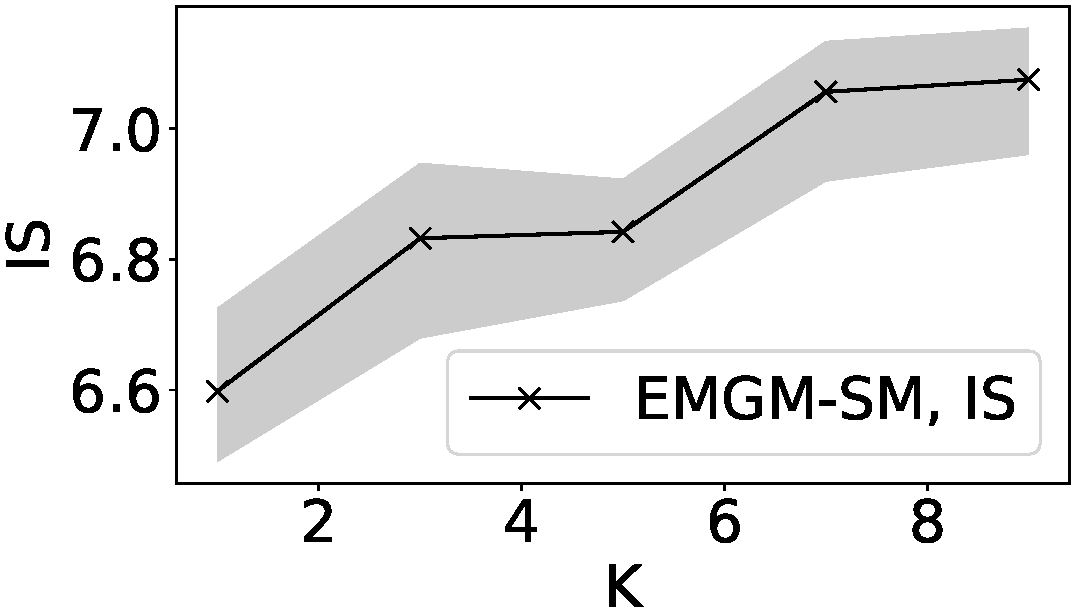
\includegraphics[width=1\linewidth]{images/mnist/scores/EMGM-NM/EMGM-NM-IS-K.pdf}
% %     \caption{IS score}
%     %     \label{fig-nm-isk}
%   \end{subfigure}
%   \vspace{-2pt}
%   \begin{subfigure}{.24\textwidth}
%     \centering
%     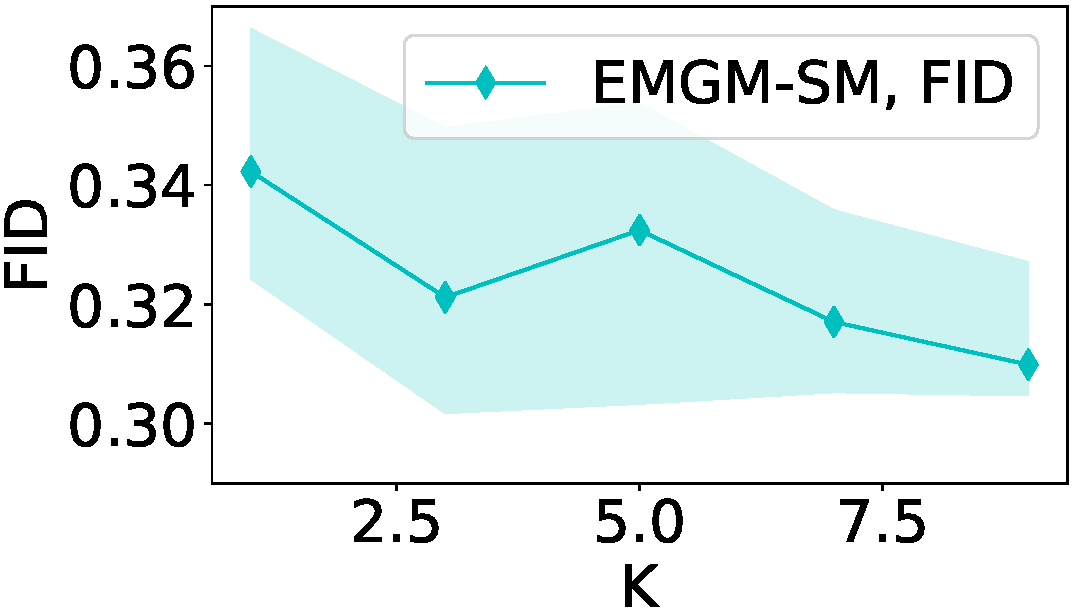
\includegraphics[width=1\linewidth]{images/mnist/scores/EMGM-NM/EMGM-NM-FID-K.pdf}
%     %     \caption{FID score}
%     %     \label{fig-nm-fidk}
%   \end{subfigure}
%   \centering
%   \begin{subfigure}{.24\textwidth}
%     \centering
%     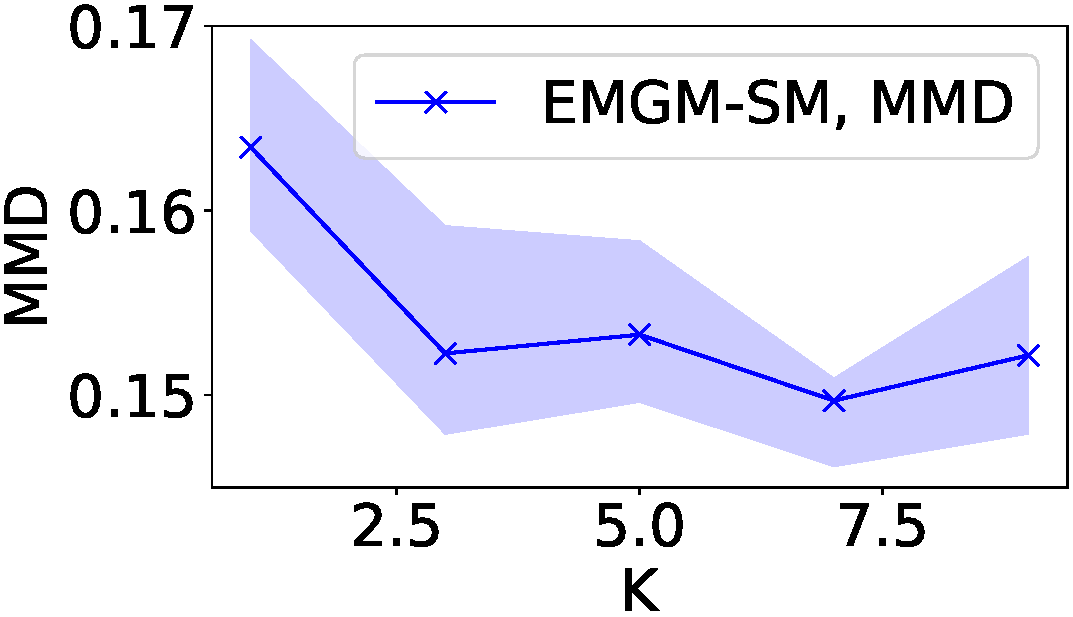
\includegraphics[width=1\linewidth]{images/mnist/scores/EMGM-NM/EMGM-NM-MMD-K.pdf}
%     %     \caption{MMD score}
%     %     \label{fig-nm-mmdk}
%   \end{subfigure}
%   \centering
%   \begin{subfigure}{0.24\textwidth}
%     \centering
%     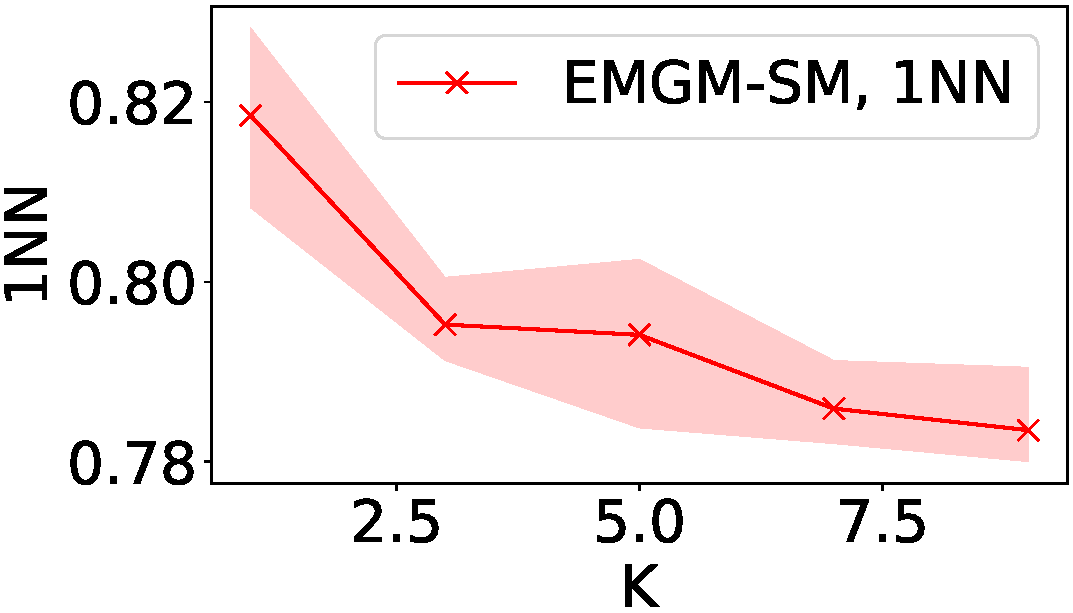
\includegraphics[width=1\linewidth]{images/mnist/scores/EMGM-NM/EMGM-NM-1NN-K.pdf}
%     %     \caption{1NN score}
%     %     \label{fig-nm-1nnk}
%   \end{subfigure}
%   \centering
%   \begin{subfigure}{.24\textwidth}
%     \centering
%     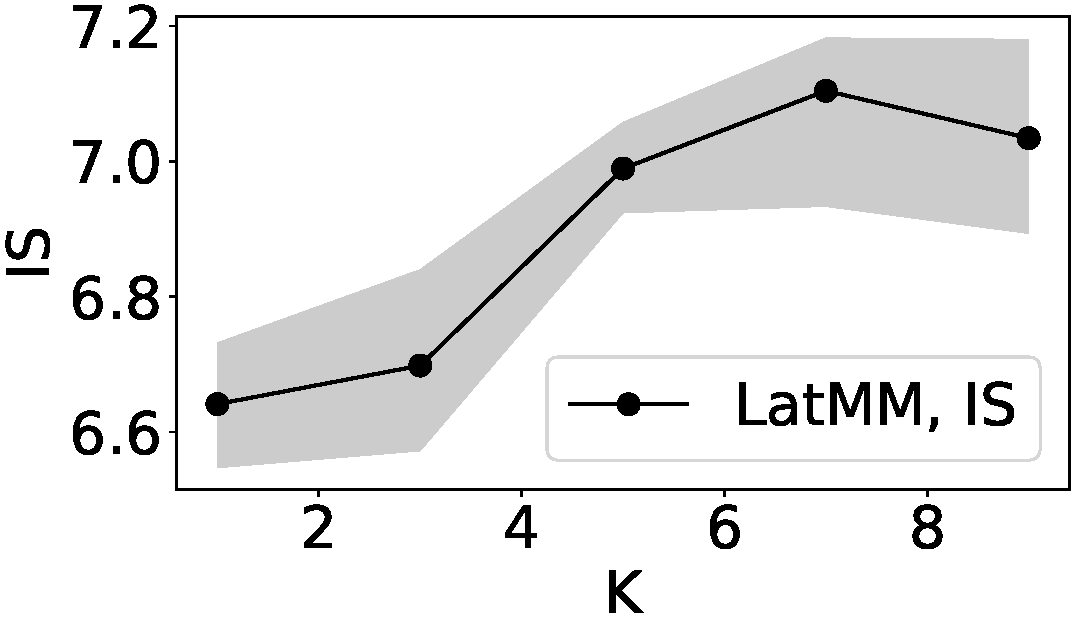
\includegraphics[width=1\linewidth]{images/mnist/scores/EMGM-SM/EMGM-SM-IS-K.pdf}
%     %     \caption{IS score}
%     %     \label{fig-sm-is}
%   \end{subfigure}
%   \centering
%   \begin{subfigure}{.24\textwidth}
%     \centering
%     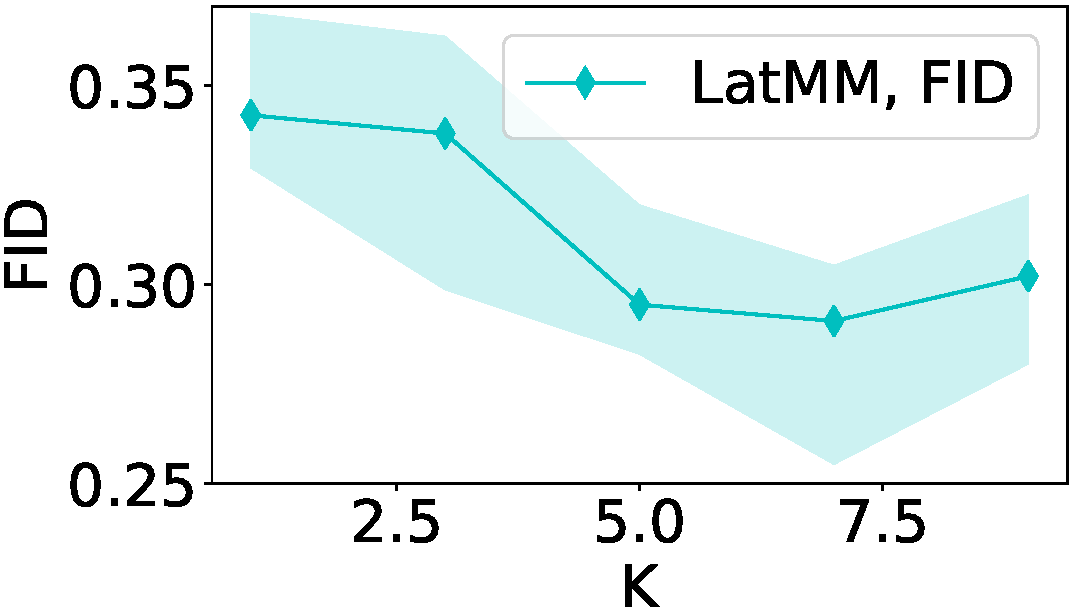
\includegraphics[width=1\linewidth]{images/mnist/scores/EMGM-SM/EMGM-SM-FID-K.pdf}
%     %     \caption{FID score}
%     %     \label{fig-sm-fid}
%   \end{subfigure}
%   \centering
%   \begin{subfigure}{.24\textwidth}
%     \centering
%     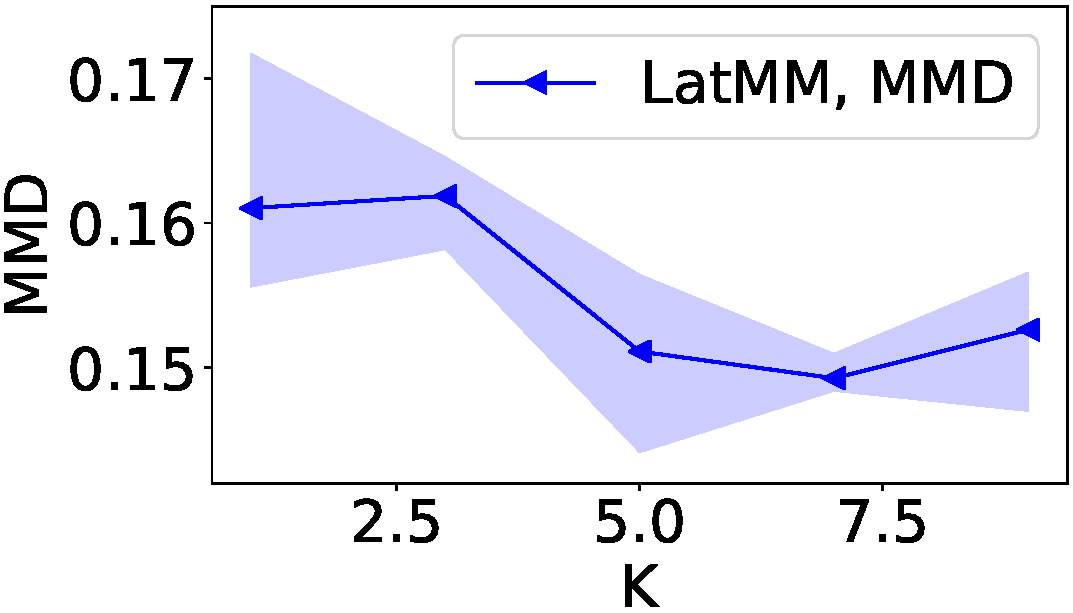
\includegraphics[width=1\linewidth]{images/mnist/scores/EMGM-SM/EMGM-SM-MMD-K.pdf}
%     %     \caption{MMD score}
%     %     \label{fig-sm-mmd}
%   \end{subfigure}
%   \begin{subfigure}{0.24\textwidth}
%     \centering
%     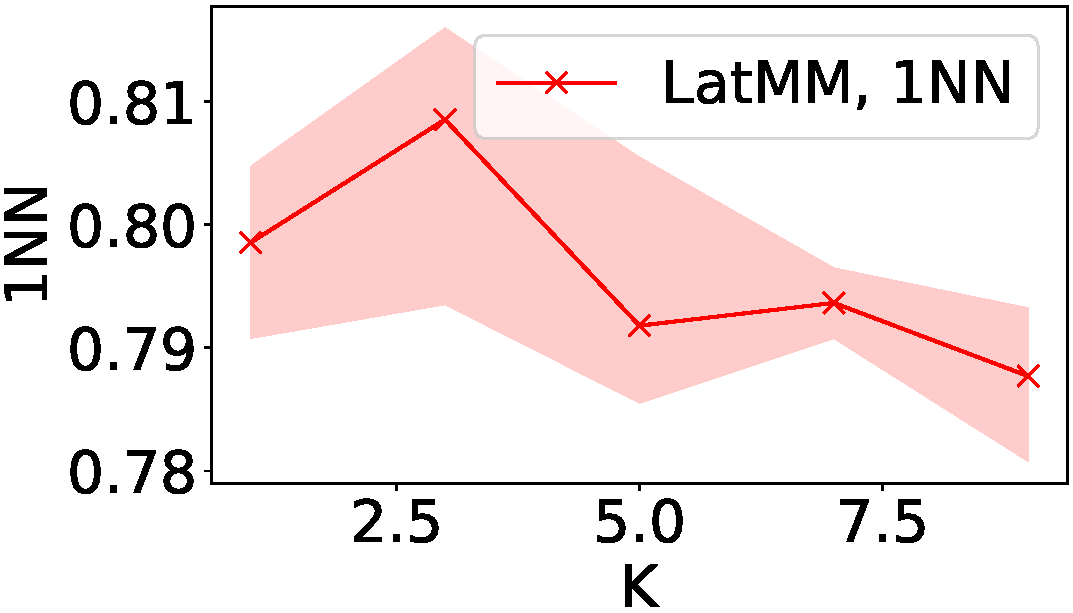
\includegraphics[width=1.\linewidth]{images/mnist/scores/EMGM-SM/EMGM-SM-1NN-K.pdf}
%     %     \caption{1NN score}
%     %     \label{fig-sm-1nn}
%   \end{subfigure}
%   \caption{IS, FID, MMD and 1NN scores of GenMM and LatMM. Evaluated
%   on $2000$ samples ($1000$ samples generated by GenMM or LatMM for
%   corresponding $K$, $1000$ samples from MNIST). $5$ experiments are
%   carried out for each assessed score at each setting of $K$. Curve
%   with marker stands for mean score and shaded area stands for the range of corresponding score. \textcolor{green}{This experiments is rechecked. Reproduced results are similar to what is shown here. (Latent standard Gaussian use standard deviation std =0.8) }}
%   \vspace{10pt}
% \end{figure*}

% \begin{figure*}[!ht]
%   \captionsetup[subfigure]{justification=centering}
%   \centering
%   \begin{subfigure}{.24\textwidth}
%     \centering
%     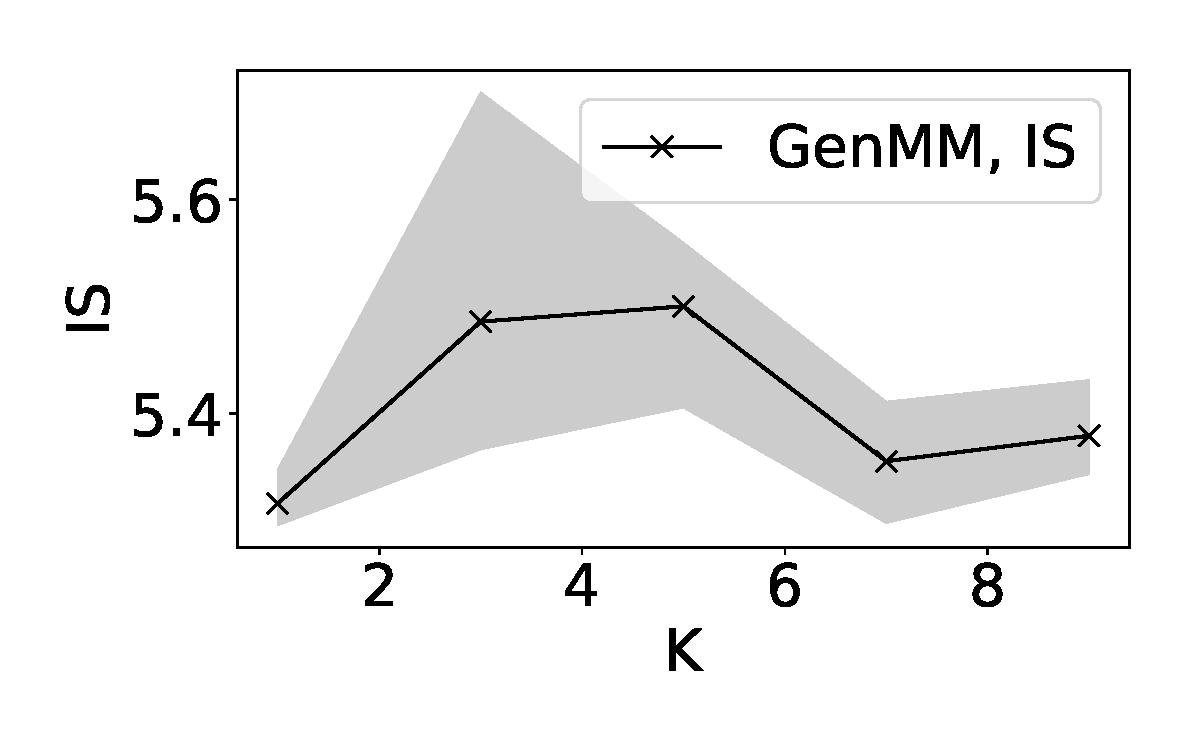
\includegraphics[width=1\linewidth]{images/fashion-mnist/scores/EMGM-NM/EMGM-NM-IS-K.pdf}
% %     \caption{IS score}
%     %     \label{fig-nm-isk}
%   \end{subfigure}
%   \vspace{-2pt}
%   \begin{subfigure}{.24\textwidth}
%     \centering
%     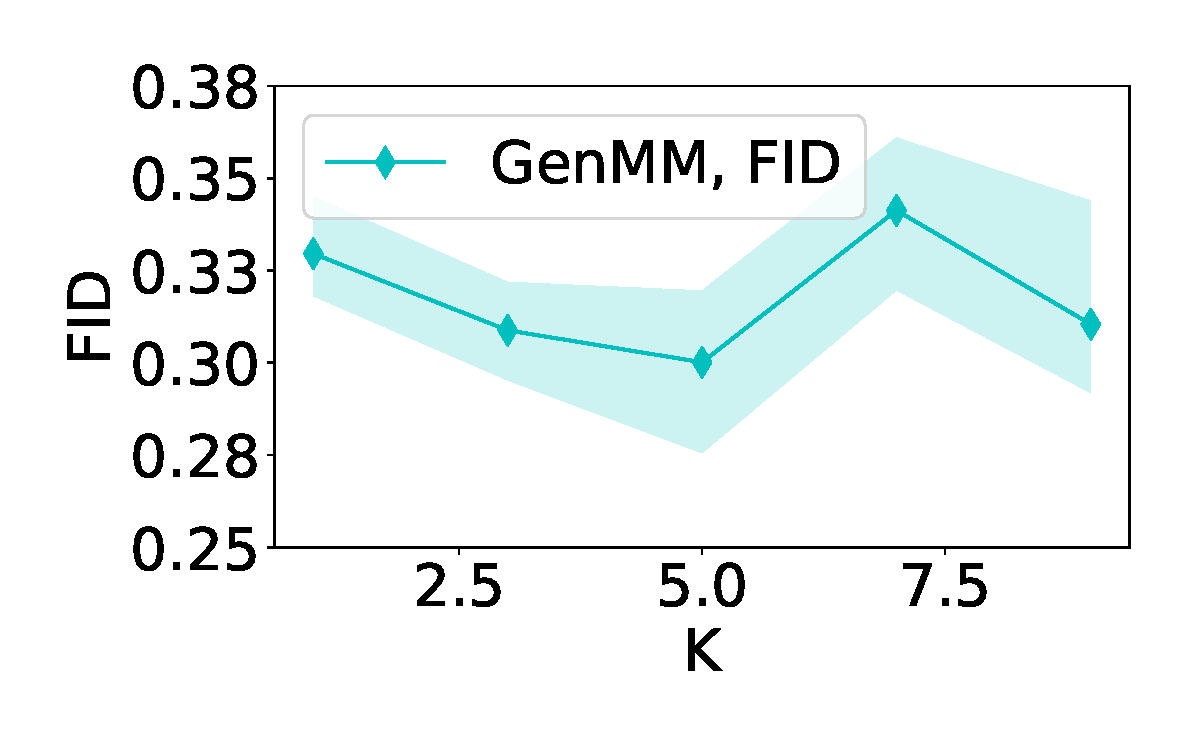
\includegraphics[width=1\linewidth]{images/fashion-mnist/scores/EMGM-NM/EMGM-NM-FID-K.pdf}
%     %     \caption{FID score}
%     %     \label{fig-nm-fidk}
%   \end{subfigure}
%   \centering
%   \begin{subfigure}{.24\textwidth}
%     \centering
%     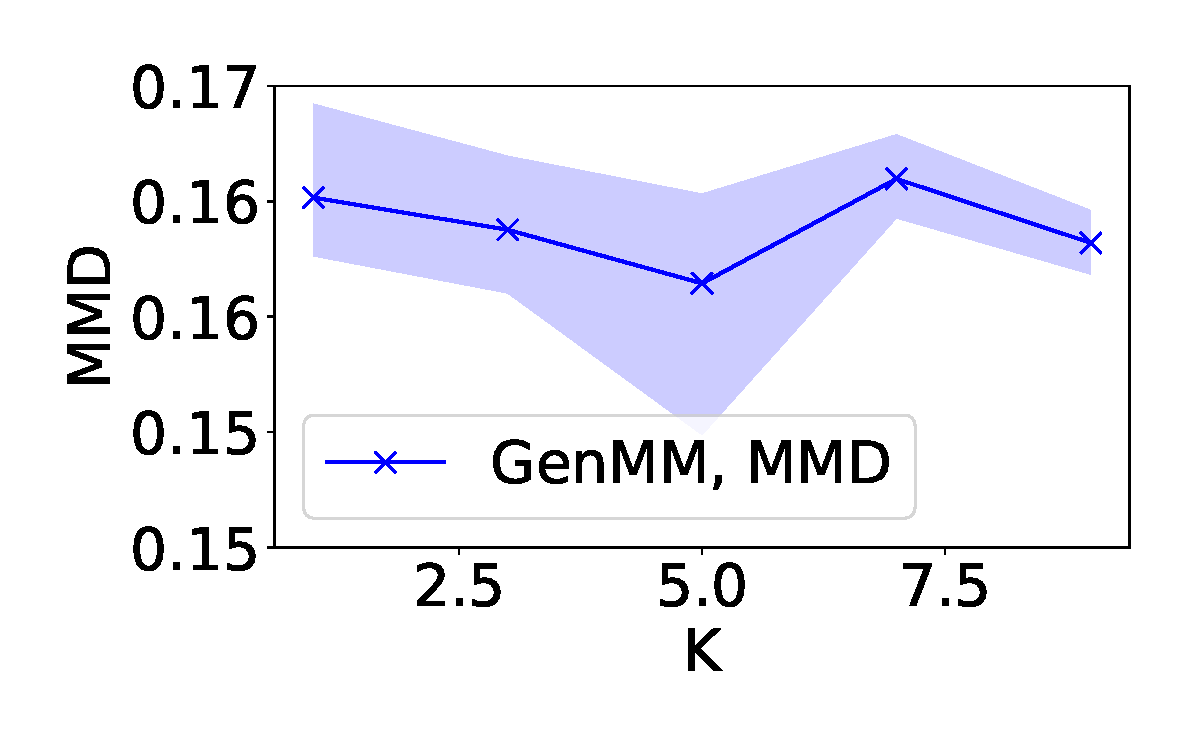
\includegraphics[width=1\linewidth]{images/fashion-mnist/scores/EMGM-NM/EMGM-NM-MMD-K.pdf}
%     %     \caption{MMD score}
%     %     \label{fig-nm-mmdk}
%   \end{subfigure}
%   \centering
%   \begin{subfigure}{0.24\textwidth}
%     \centering
%     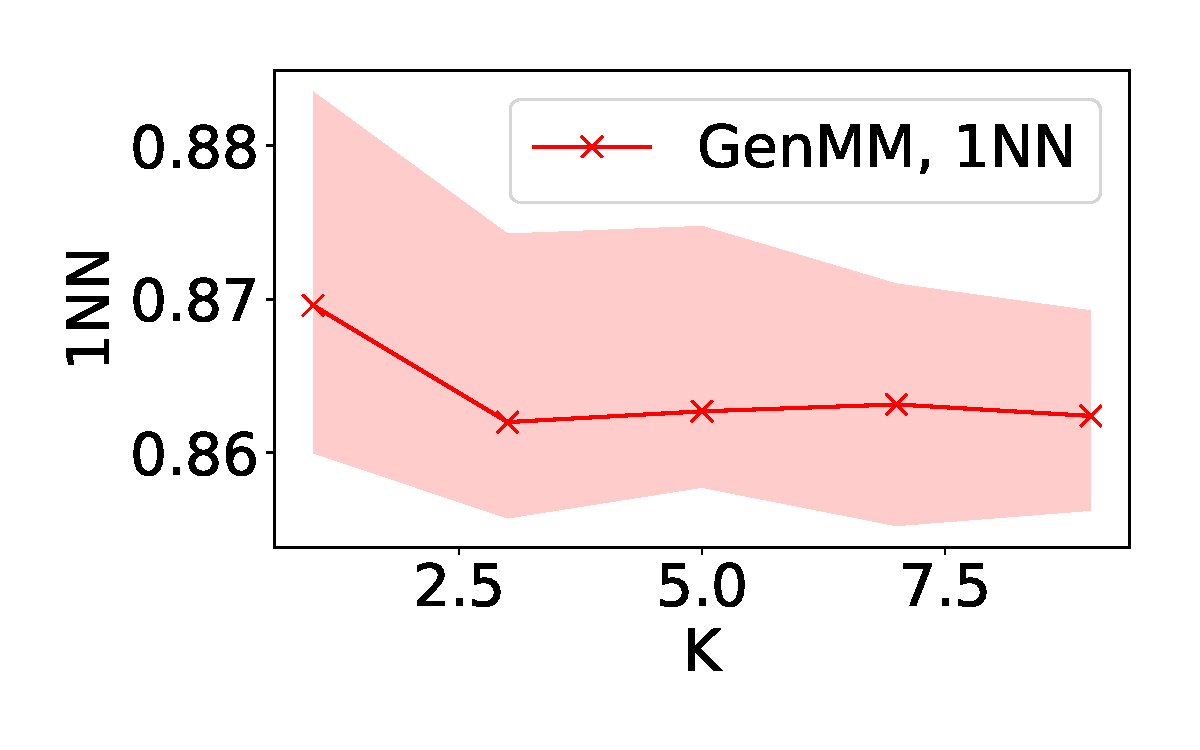
\includegraphics[width=1\linewidth]{images/fashion-mnist/scores/EMGM-NM/EMGM-NM-1NN-K.pdf}
%     %     \caption{1NN score}
%     %     \label{fig-nm-1nnk}
%   \end{subfigure}
%   \centering
%   \begin{subfigure}{.24\textwidth}
%     \centering
%     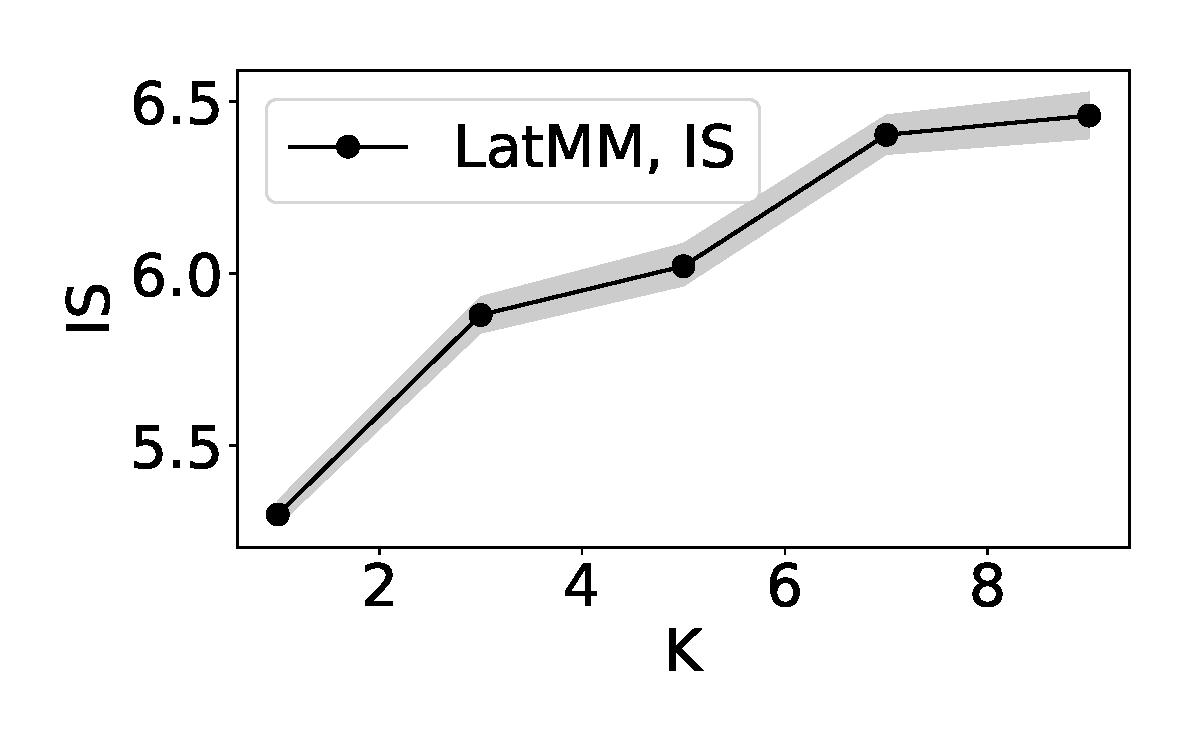
\includegraphics[width=1\linewidth]{images/fashion-mnist/scores/EMGM-SM/EMGM-SM-IS-K.pdf}
%     %     \caption{IS score}
%     %     \label{fig-sm-is}
%   \end{subfigure}
%   \centering
%   \begin{subfigure}{.24\textwidth}
%     \centering
%     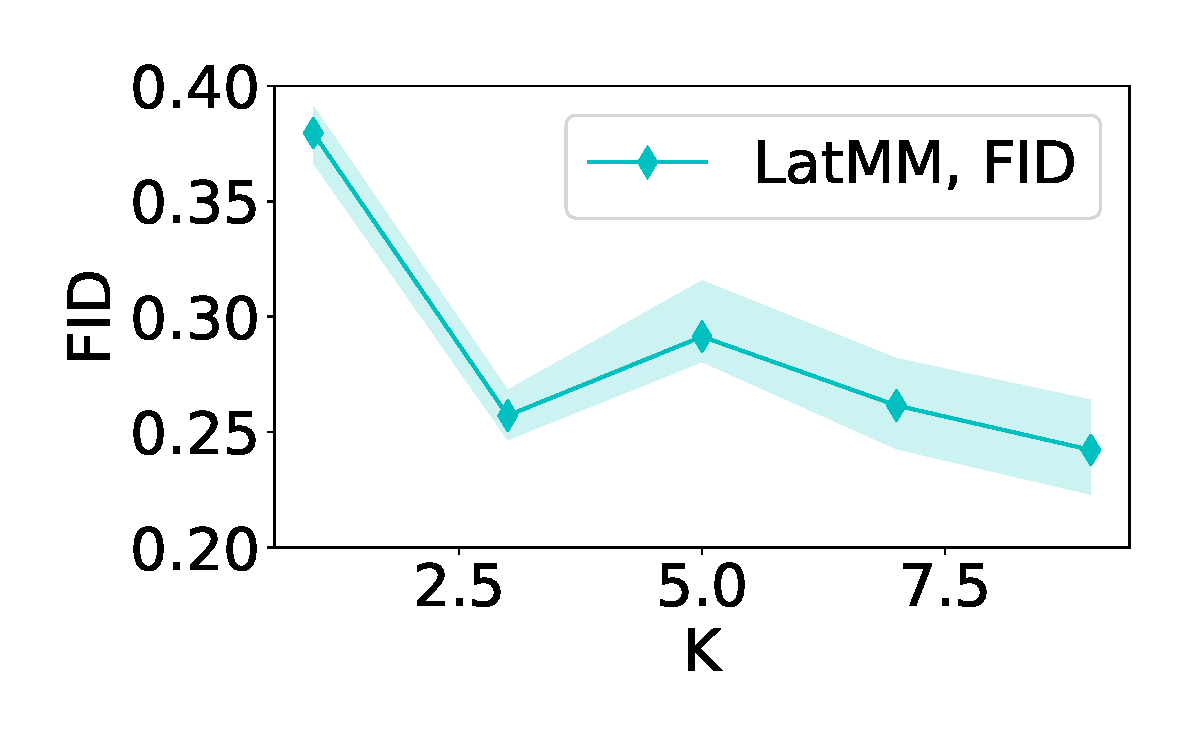
\includegraphics[width=1\linewidth]{images/fashion-mnist/scores/EMGM-SM/EMGM-SM-FID-K.pdf}
%     %     \caption{FID score}
%     %     \label{fig-sm-fid}
%   \end{subfigure}
%   \centering
%   \begin{subfigure}{.24\textwidth}
%     \centering
%     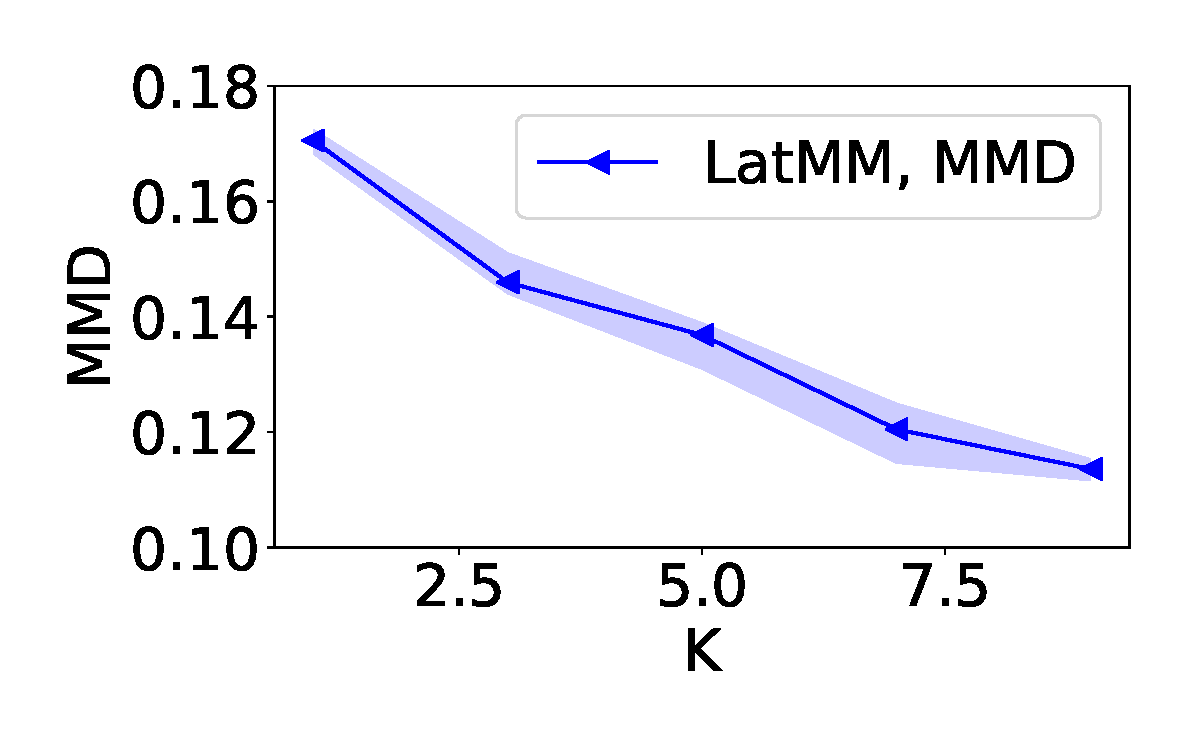
\includegraphics[width=1\linewidth]{images/fashion-mnist/scores/EMGM-SM/EMGM-SM-MMD-K.pdf}
%     %     \caption{MMD score}
%     %     \label{fig-sm-mmd}
%   \end{subfigure}
%   \begin{subfigure}{0.24\textwidth}
%     \centering
%     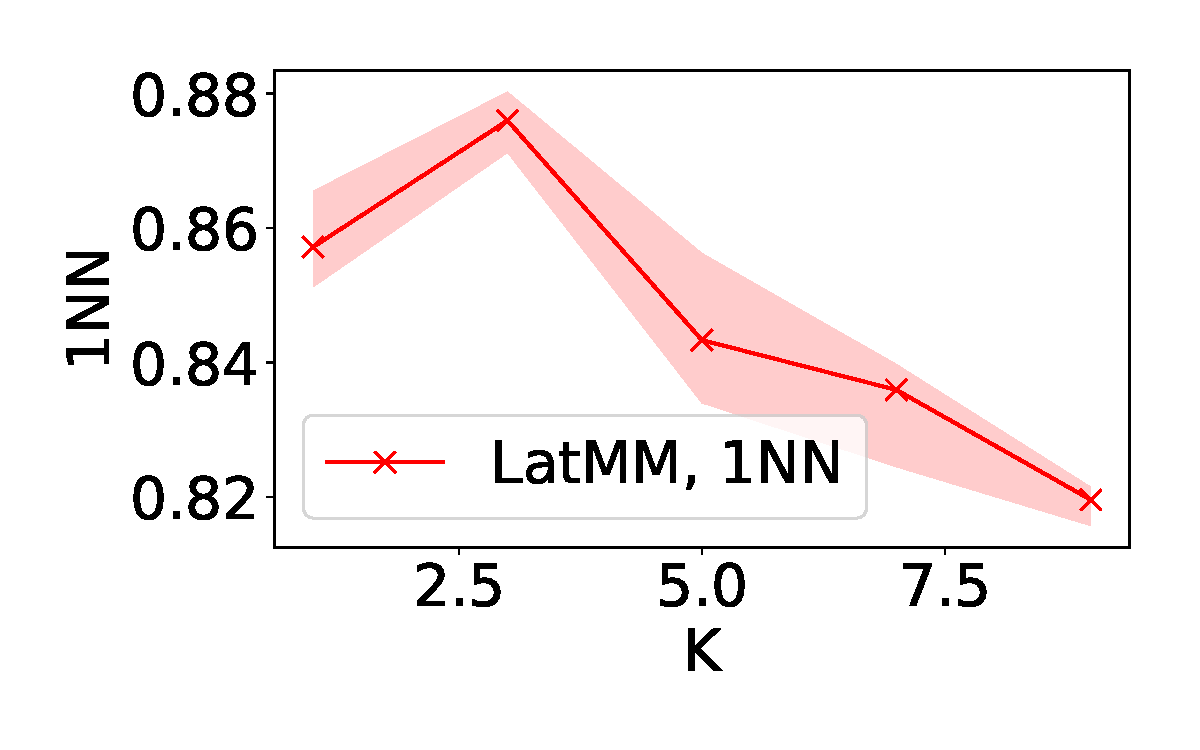
\includegraphics[width=1.\linewidth]{images/fashion-mnist/scores/EMGM-SM/EMGM-SM-1NN-K.pdf}
%     %     \caption{1NN score}
%     %     \label{fig-sm-1nn}
%   \end{subfigure}
%   \caption{ GenMM and LatMM evaluated on Fashion-MNIST (std =0.8) }
%   \vspace{10pt}
% \end{figure*}



In this section, we evaluate our proposed mixture models for generating samples and maximum likelihood classification. We will show encouraging results.

    %     under different metrics firstly. Then demos of sample generating and interpolation are shown. Lastly, we apply our model to classification tasks based on maximum likelihood criterion.

\begin{figure*}[!ht]
  \captionsetup[subfigure]{justification=centering}
  \centering
  \begin{subfigure}{.4\textwidth}
    \centering
    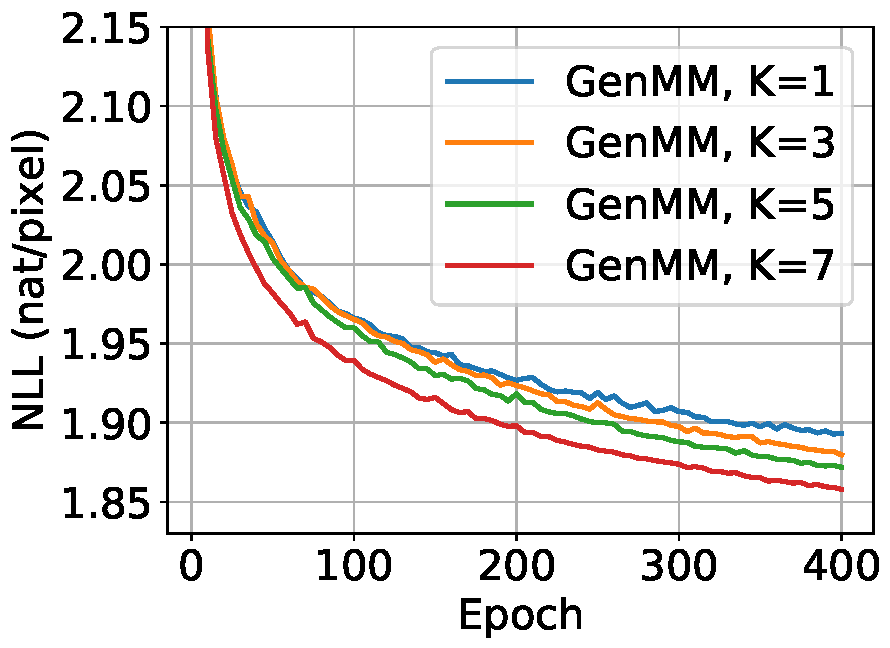
\includegraphics[width=1\linewidth]{images/supply/mnist_GenMM_nll_curves-crop.pdf}
    \vspace{-0.6cm}
    \caption{Dataset MNIST}
    \label{fig-genmm-mnist-nll-curve}
  \end{subfigure}\hspace{1cm}
  \begin{subfigure}{.4\textwidth}
    \centering
    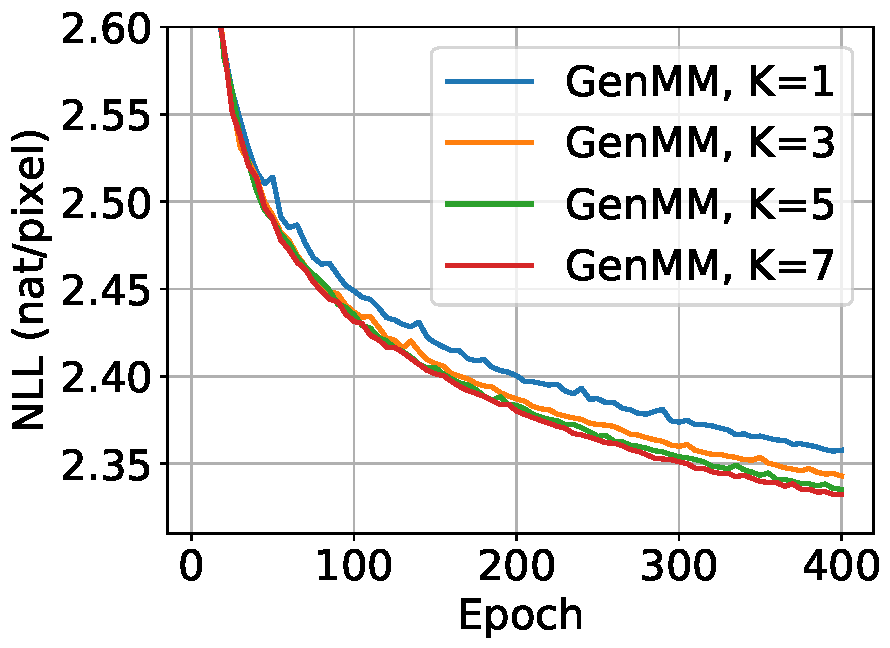
\includegraphics[width=1\linewidth]{images/supply/fashion_GenMM_nll_curves-crop.pdf}
    \vspace{-0.6cm}
    \caption{Dataset Fashion-MNIST}
    \label{fig-genmm-fsh-nll-curve}
  \end{subfigure}
  \vspace{-0.3cm}
  \caption{NLL (Unit: nat/pixel) of GenMM versus training epochs with different number of mixture component $k$. (a) $10000$ images from MNIST is used for training, (b) $10000$ images from Fashion-MNIST is used for training.}
  \label{fig:genmm-nll}
\end{figure*}

\begin{figure*}[!ht]
  \captionsetup[subfigure]{justification=centering}
  \centering
  \begin{subfigure}{.4\textwidth}
    \centering
    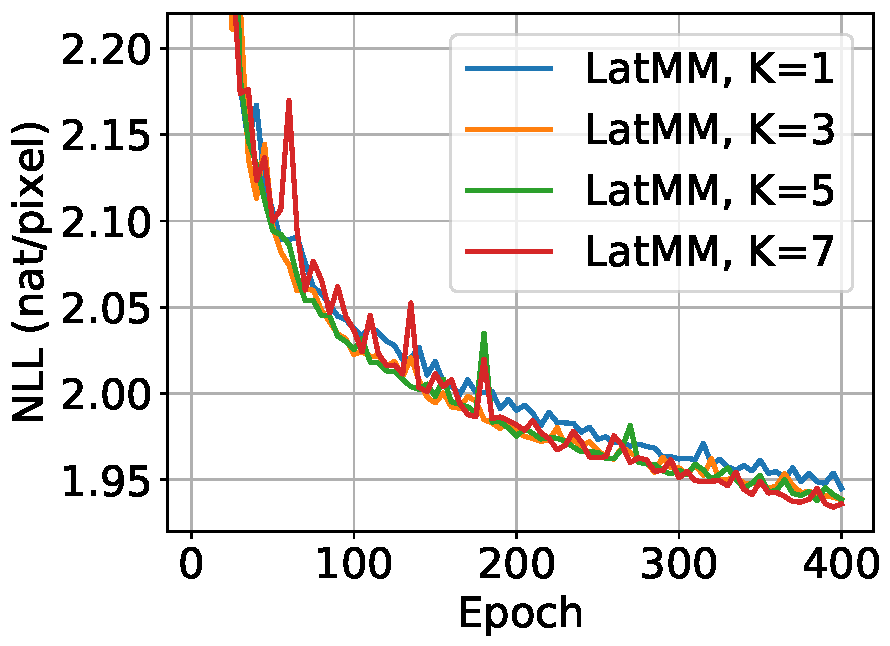
\includegraphics[width=1\linewidth]{images/supply/mnist_LatMM_nll_curves-crop.pdf}
    \vspace{-0.6cm}
    \caption{Dataset of MNIST}
    \label{fig-latmm-mnist-nll-curve}
  \end{subfigure}\hspace{1cm}
  \begin{subfigure}{.4\textwidth}
    \centering
    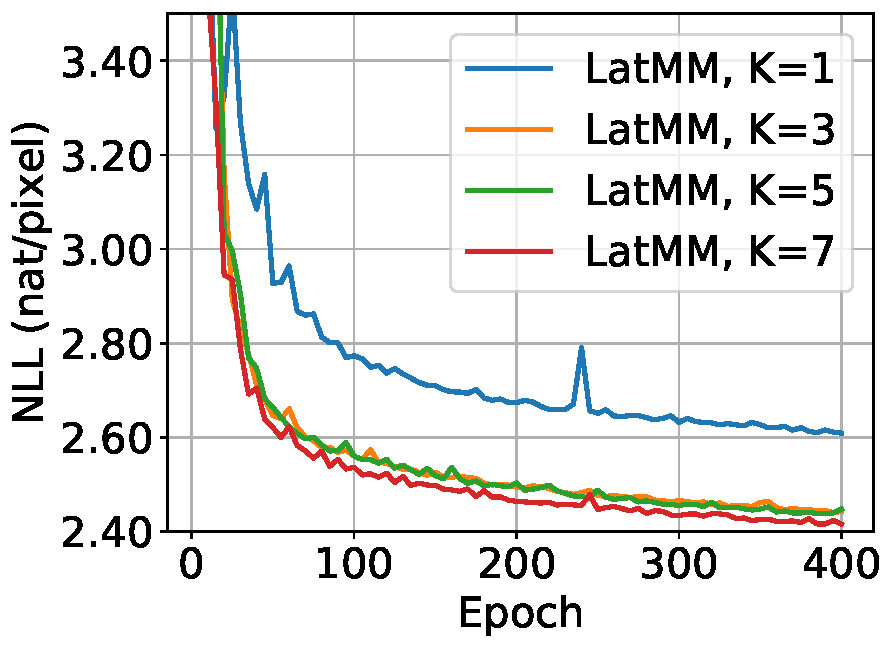
\includegraphics[width=1\linewidth]{images/supply/fashion_LatMM_nll_curves-crop.pdf}
    \vspace{-0.6cm}
    \caption{Dataset Fashion-MNIST}
    \label{fig-latmm-fsh-nll-curve}
  \end{subfigure}
  \vspace{-0.3cm}
  \caption{NLL (Unit: nat/pixel) of LatMM versus training epochs with different number of mixture component $k$. (a) $10000$ images from MNIST is used for training, (b) $10000$ images from Fashion-MNIST is used for training.}
  \label{fig:latmm-nll}
  \vspace{0.3cm}
\end{figure*}
\subsection{Experimental setup}\label{sub:exp-setup}



We use the flow-based neural network for implementing generators $\{\bm{g}_k\}_{k=1}^{K}$ in GenMM and $\bm{g}$ in LatMM. Specifically, we use the Glow structure \cite{2018arXiv180703039K} that is developed based on RealNVP \cite{2016arXiv160508803D} and NICE \cite{DBLP:journals/corr/DinhKB14}. As introduced in \autoref{subsec-flow-intro}, the operation in \autoref{eq-gl} is a coupling
layer. Since only a part of the input is mapped non-linearly after a coupling
layer and the rest part remains the same, permutation \cite{2016arXiv160508803D} or $1\times 1$ convolution operation \cite{2018arXiv180703039K} is used to alternate the part of signal that goes through identity mapping. In Glow structure, a basic \textit{flow step} is the concatenation of three layers: Actnorm (element-wise affine mapping)
$\rightarrow$ $1\times 1$ Convolution (for permutation purpose)
$\rightarrow$ Coupling layer. A \textit{flow block} consists of: a squeeze layer,
several flow steps, a split layer. A squeeze layer reshapes
signal. A split layer allows
flow model to split some elements of hidden layers out and model them
directly as standard Gaussian, which relieves computation burden. In our experiments, there are also split layers that make dimension of $\bm{z}$ one fourth of dimension $\bm{x}$, and split signal in hidden layers are modeled as standard Gaussian. 

    %     In all of our experiments, the generators $\bm{g}_k, \forall k$, in
    %     GenMM and $\bm{g}$ of LatMM use the same structure: \textit{three} flow blocks with
    %     each flow block consisting of \textit{four} coupling layers.  
All generators used in our experiments are randomly initialized before training. 
    %     In order to make comparison fair, our models with different configuration of $K$ are all trained for $30$ epochs on both datasets. Comparison are made with the trained models.  
In addition, the prior distribution $\bm{\pi}$ update in both GenMM and LatMM is every $5$ epochs, {i.e.},  $t_{\pi} = 5$. For the training of LatMM, we adopt the Gamma distribution $\Gamma(\bm{\sigma}_k^{-1}; a, b)$ as the parameter prior for $\bm{\sigma}_k^{-1}, \forall k$, with shape parameter $a=2$ and rate parameter $b = 1$.
Our models are implemented using Pytorch and experiments are carried out on Tesla P100 GPU. Code is available at github repository\footnote{https://github.com/FirstHandScientist/EM-GM}.


\begin{figure*}[!tp]
  \captionsetup[subfigure]{justification=centering}
  \centering
  \begin{subfigure}{.24\textwidth}
    \centering
    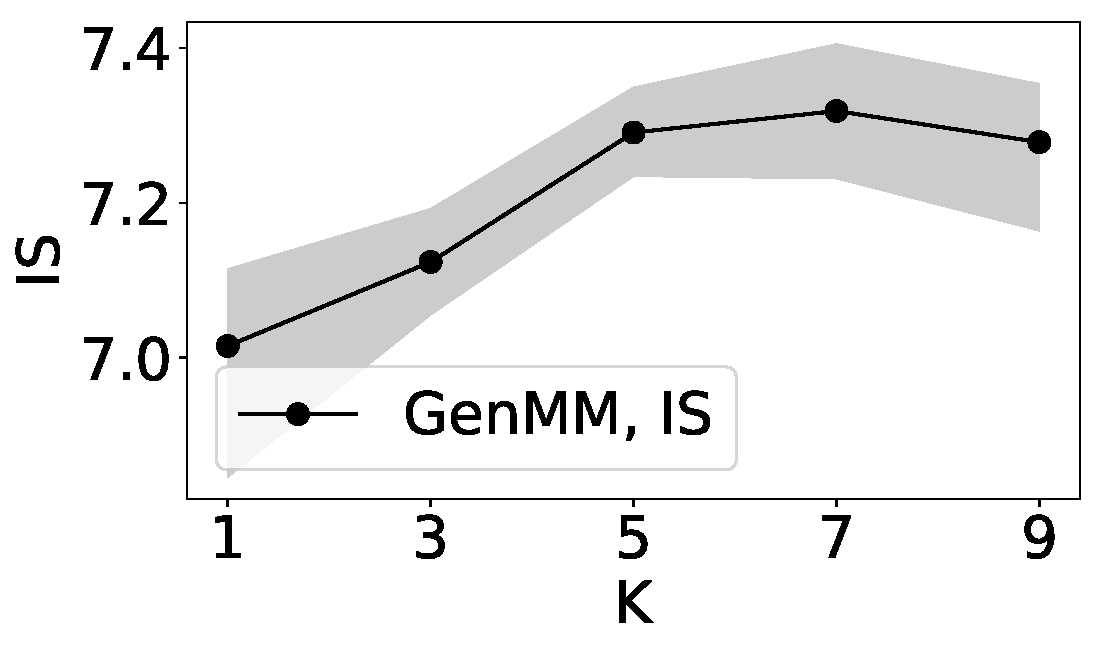
\includegraphics[width=1\linewidth]{images/mnist/scores/std1EMGM-NM/EMGM-NM-IS-K.pdf}
    % \caption{IS score}
    % \label{fig-nm-isk}
  \end{subfigure}
  \vspace{-2pt}
  \begin{subfigure}{.24\textwidth}
    \centering
    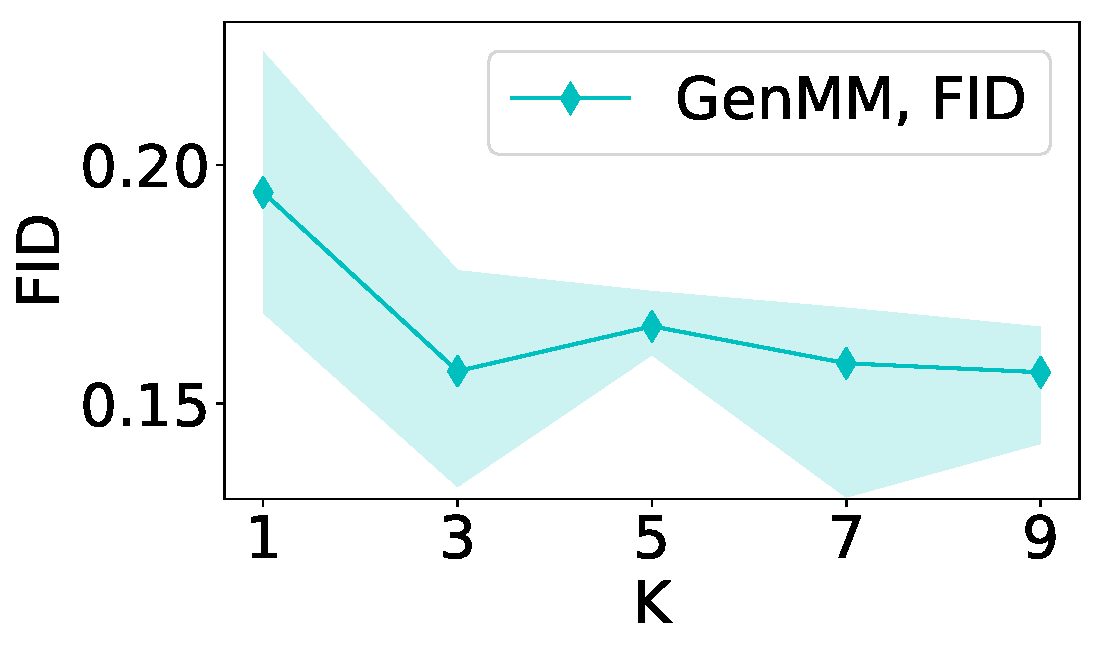
\includegraphics[width=1\linewidth]{images/mnist/scores/std1EMGM-NM/EMGM-NM-FID-K.pdf}
    % \caption{FID score}
    % \label{fig-nm-fidk}
  \end{subfigure}
  \centering
  \begin{subfigure}{.24\textwidth}
    \centering
    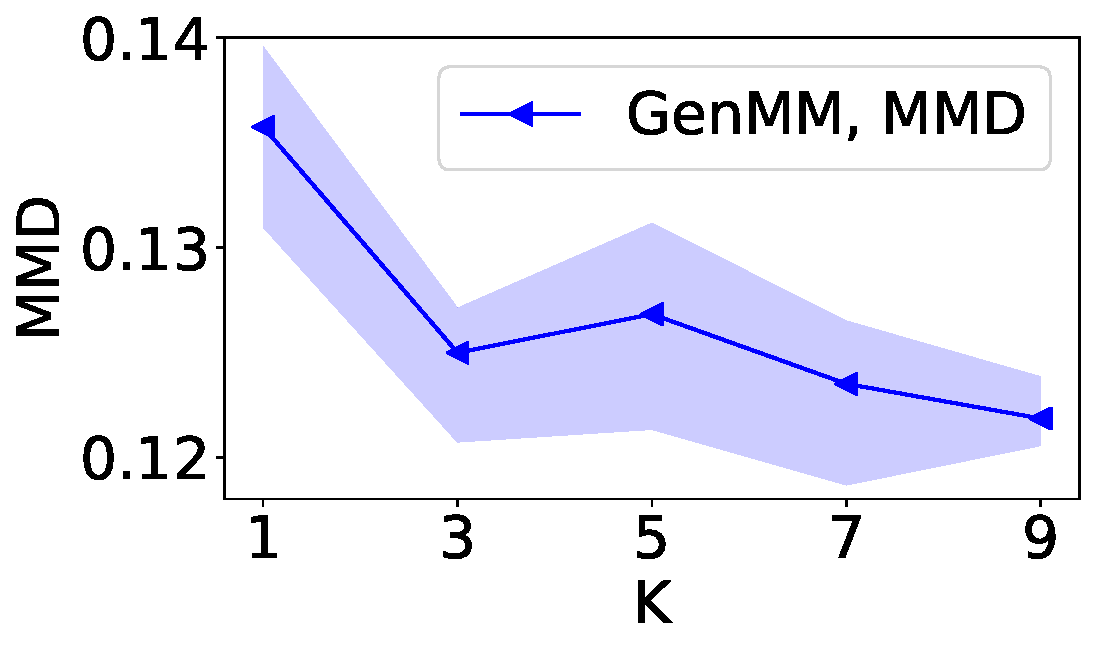
\includegraphics[width=1\linewidth]{images/mnist/scores/std1EMGM-NM/EMGM-NM-MMD-K.pdf}
    % \caption{MMD score}
    % \label{fig-nm-mmdk}
  \end{subfigure}
  \centering
  \begin{subfigure}{0.24\textwidth}
    \centering
    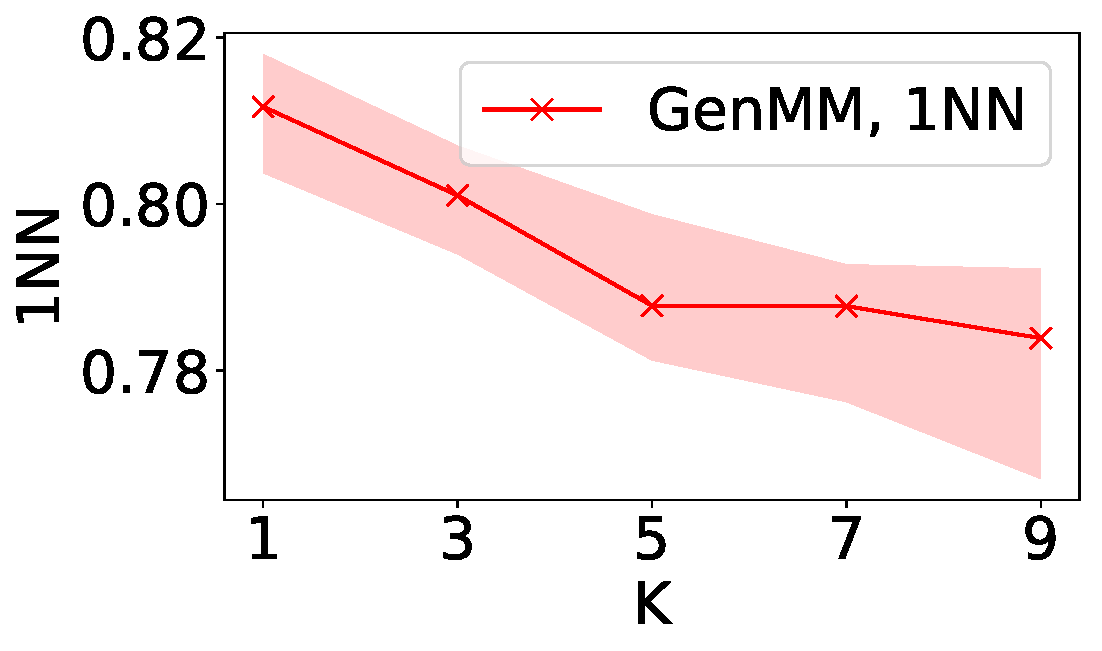
\includegraphics[width=1\linewidth]{images/mnist/scores/std1EMGM-NM/EMGM-NM-1NN-K.pdf}
    % \caption{1NN score}
    % \label{fig-nm-1nnk}
  \end{subfigure}
  \centering
  \begin{subfigure}{.24\textwidth}
    \centering
    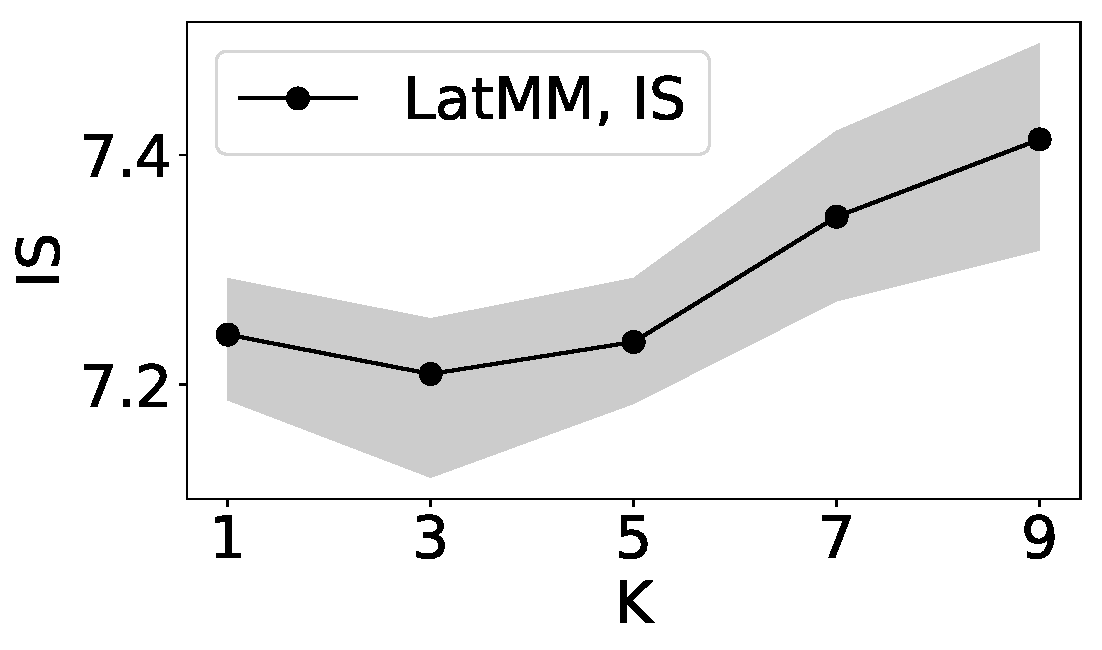
\includegraphics[width=1\linewidth]{images/mnist/scores/std1EMGM-SM/EMGM-SM-IS-K.pdf}
    % \caption{IS score}
    % \label{fig-sm-is}
  \end{subfigure}
  \centering
  \begin{subfigure}{.24\textwidth}
    \centering
    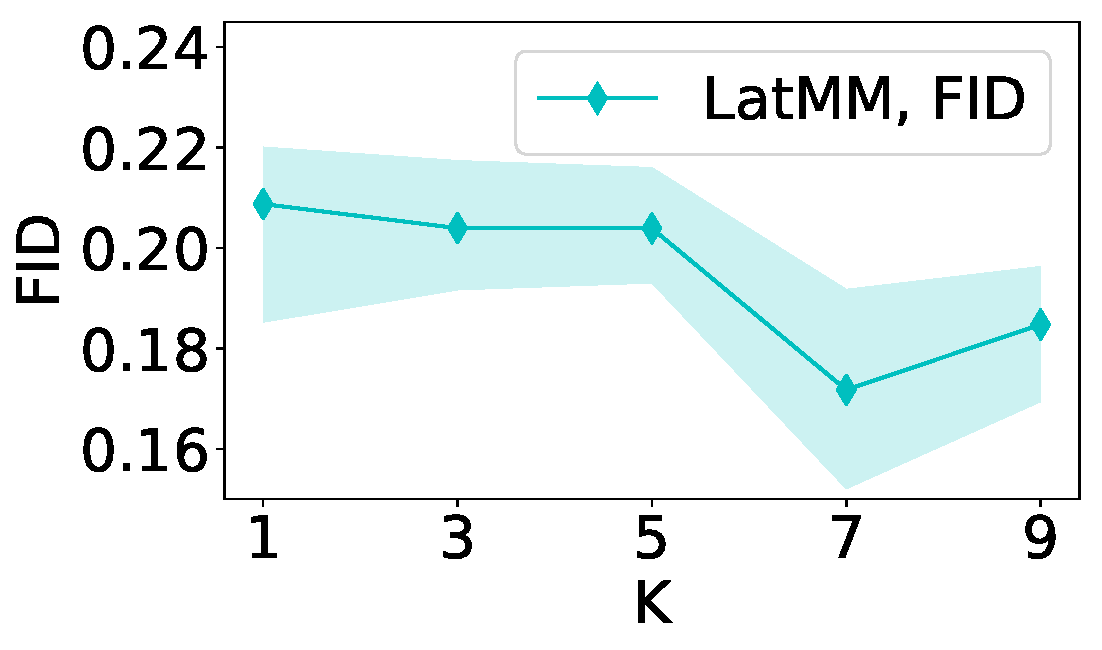
\includegraphics[width=1\linewidth]{images/mnist/scores/std1EMGM-SM/EMGM-SM-FID-K.pdf}
    % \caption{FID score}
    % \label{fig-sm-fid}
  \end{subfigure}
  \centering
  \begin{subfigure}{.24\textwidth}
    \centering
    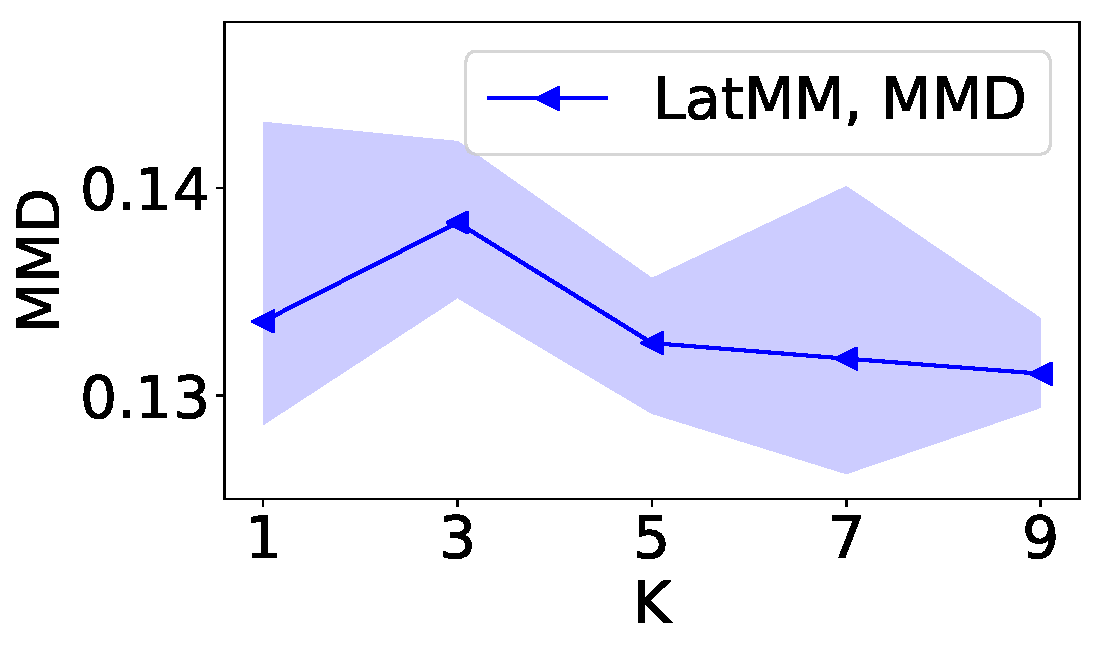
\includegraphics[width=1\linewidth]{images/mnist/scores/std1EMGM-SM/EMGM-SM-MMD-K.pdf}
    % \caption{MMD score}
    % \label{fig-sm-mmd}
  \end{subfigure}
  \begin{subfigure}{0.24\textwidth}
    \centering
    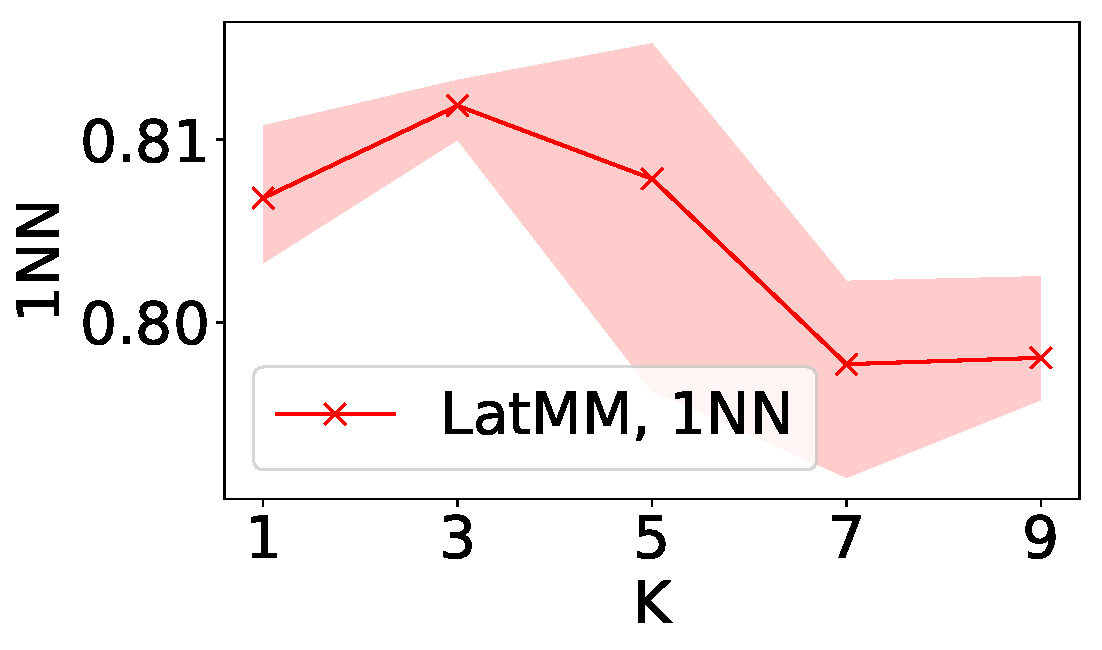
\includegraphics[width=1.\linewidth]{images/mnist/scores/std1EMGM-SM/EMGM-SM-1NN-K.pdf}
    % \caption{1NN score}
    % \label{fig-sm-1nn}
  \end{subfigure}
  \vspace{-0.35cm}
  \caption{IS, FID, MMD and 1NN of GenMM and LatMM for MNIST dataset. GenMM and LatMM are trained on $60000$ images of MNIST. The results are evaluated on $2000$ samples per simulation point ($1000$ samples generated by GenMM or LatMM for corresponding $K$, $1000$ samples from MNIST). $5$ experiments are carried out for each assessed score at each setting of $K$. Curve with marker denotes mean score and shaded area denotes the range of corresponding score.}\label{fig-scores-k}
  % \vspace{10pt}
  \vspace{-0.15cm}
\end{figure*}

\begin{figure*}[!ht]
  \captionsetup[subfigure]{justification=centering}
  \centering
  \begin{subfigure}{.24\textwidth}
    \centering
    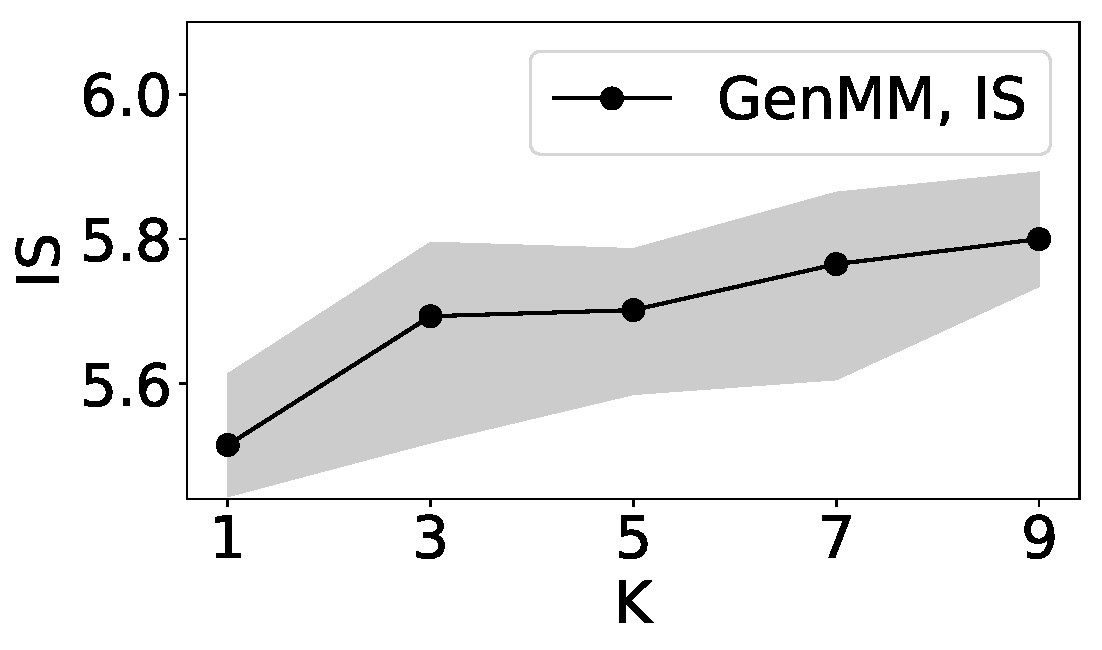
\includegraphics[width=1.0\linewidth]{images/fashion-mnist/scores/std1EMGM-NM/EMGM-NM-IS-K.pdf}
    % \caption{IS score}
    % \label{fig-nm-isk}
  \end{subfigure}
  \vspace{-2pt}
  \begin{subfigure}{.24\textwidth}
    \centering
    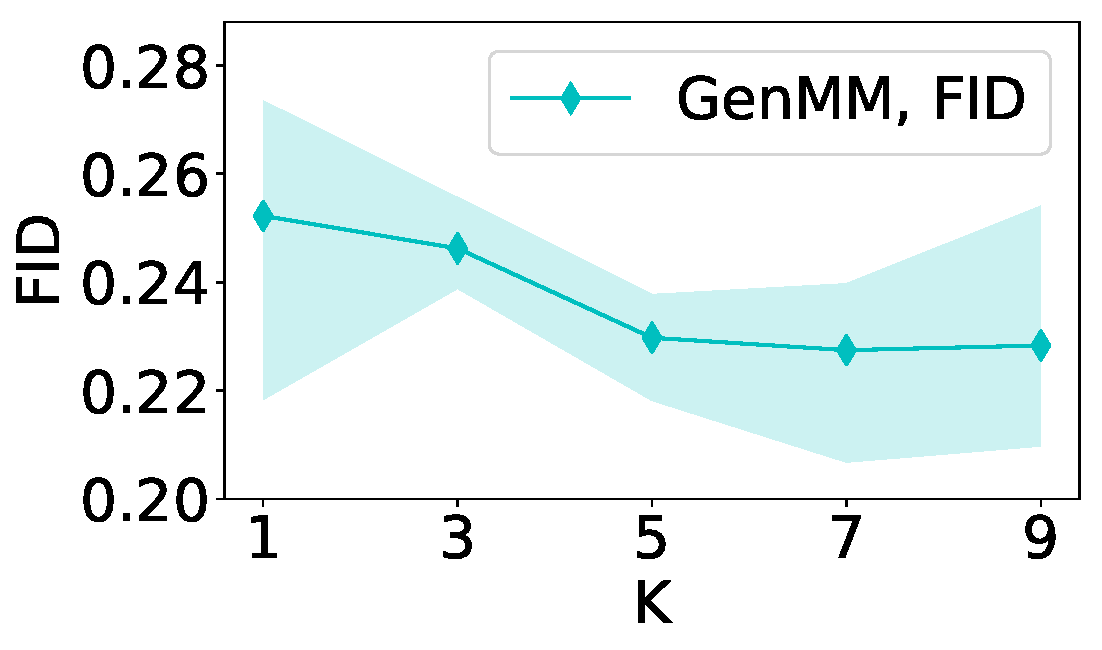
\includegraphics[width=1.0\linewidth]{images/fashion-mnist/scores/std1EMGM-NM/EMGM-NM-FID-K.pdf}
    % \caption{FID score}
    % \label{fig-nm-fidk}
  \end{subfigure}
  \centering
  \begin{subfigure}{.24\textwidth}
    \centering
    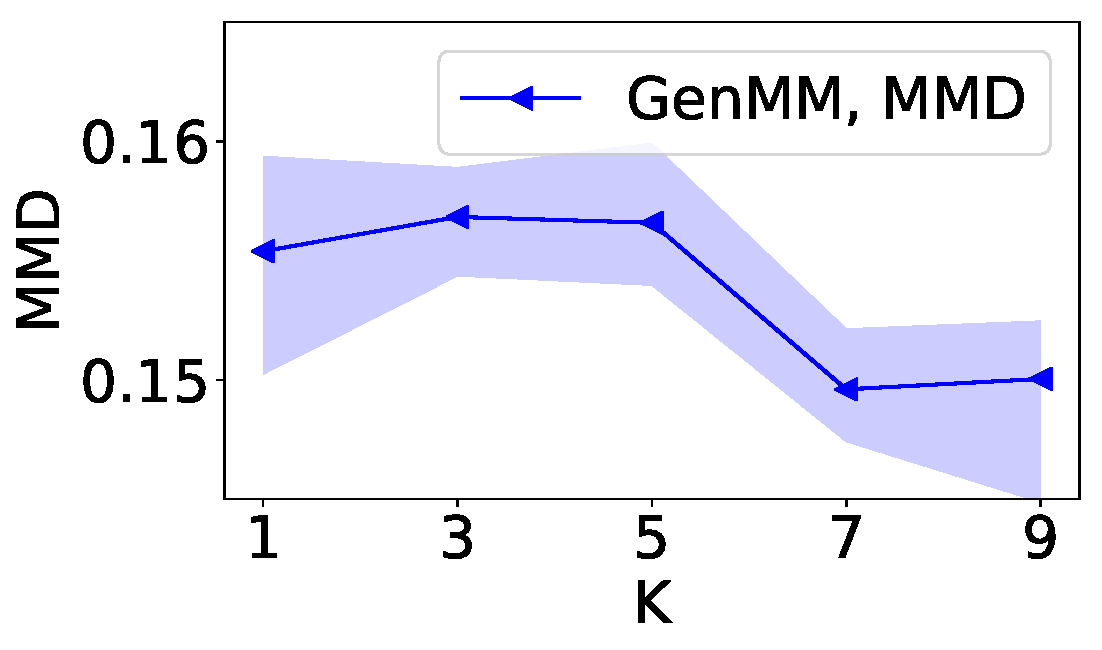
\includegraphics[width=1\linewidth]{images/fashion-mnist/scores/std1EMGM-NM/EMGM-NM-MMD-K.pdf}
    % \caption{MMD score}
    % \label{fig-nm-mmdk}
  \end{subfigure}
  \centering
  \begin{subfigure}{0.24\textwidth}
    \centering
    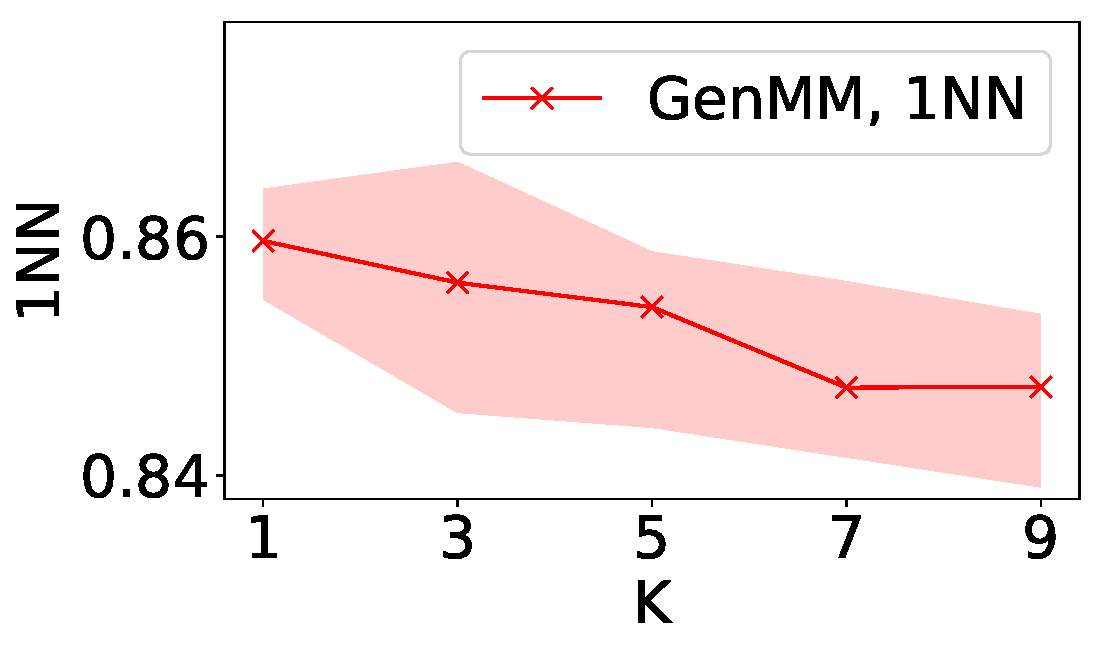
\includegraphics[width=1\linewidth]{images/fashion-mnist/scores/std1EMGM-NM/EMGM-NM-1NN-K.pdf}
    % \caption{1NN score}
    % \label{fig-nm-1nnk}
  \end{subfigure}
  \centering
  \begin{subfigure}{.24\textwidth}
    \centering
    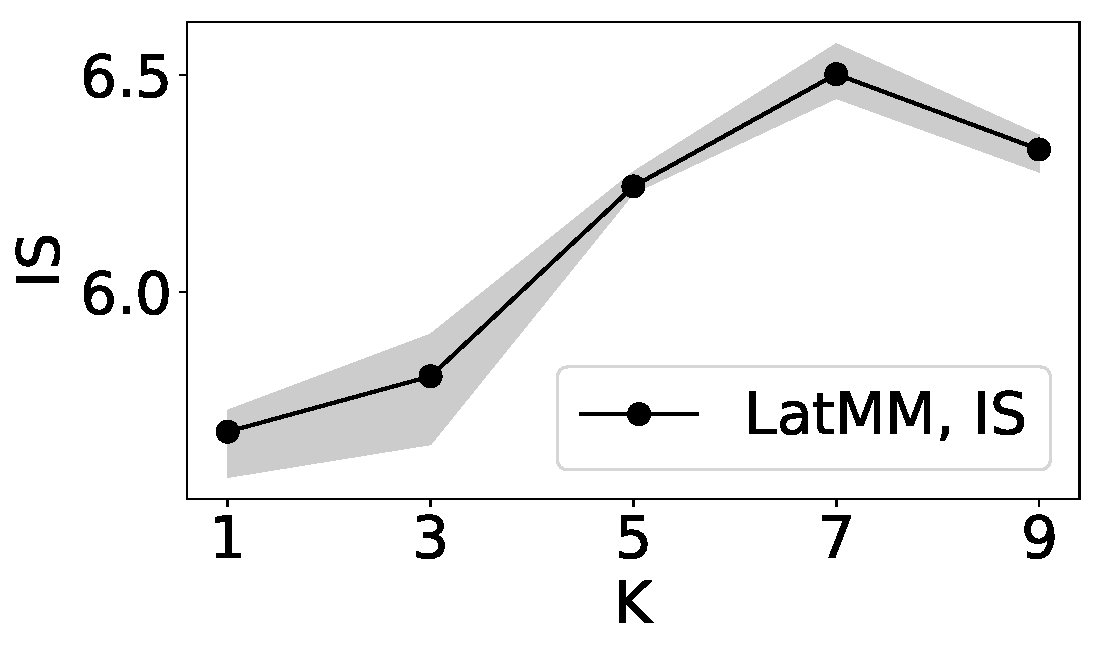
\includegraphics[width=1\linewidth]{images/fashion-mnist/scores/std1EMGM-SM/EMGM-SM-IS-K.pdf}
    % \caption{IS score}
    % \label{fig-sm-is}
  \end{subfigure}
  \centering
  \begin{subfigure}{.24\textwidth}
    \centering
    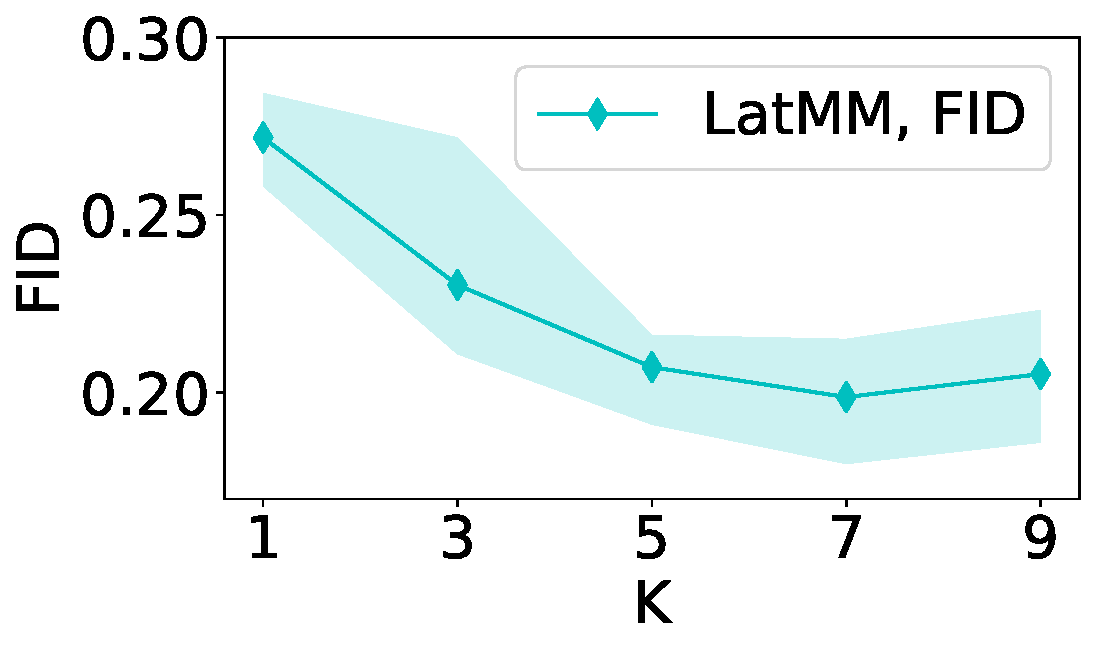
\includegraphics[width=1\linewidth]{images/fashion-mnist/scores/std1EMGM-SM/EMGM-SM-FID-K.pdf}
    % \caption{FID score}
    % \label{fig-sm-fid}
  \end{subfigure}
  \centering
  \begin{subfigure}{.24\textwidth}
    \centering
    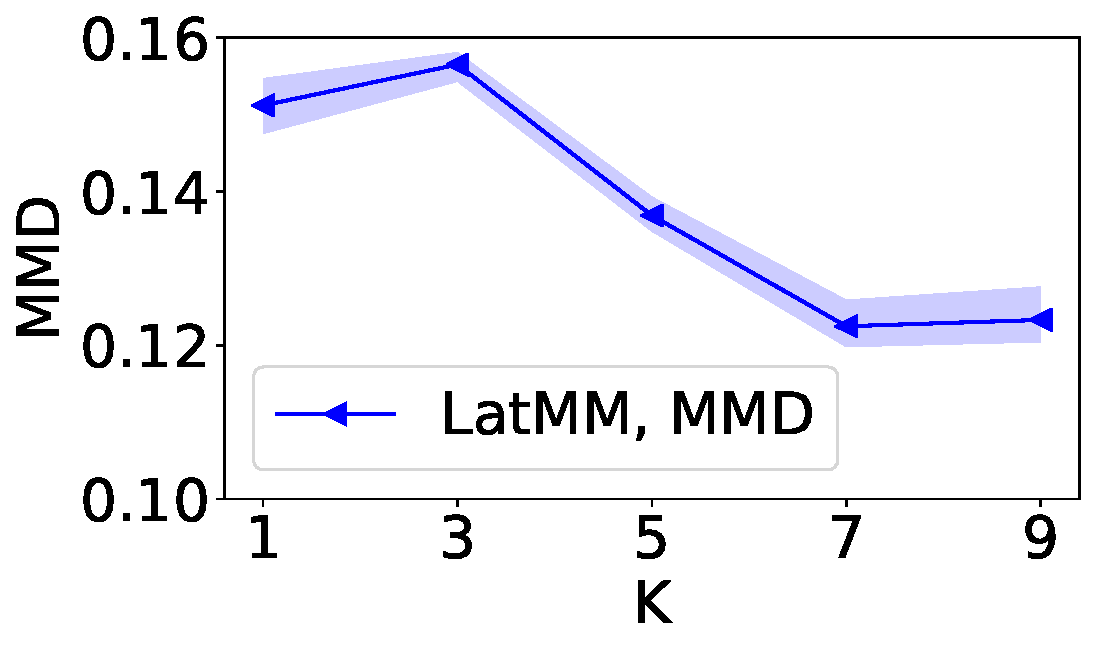
\includegraphics[width=1\linewidth]{images/fashion-mnist/scores/std1EMGM-SM/EMGM-SM-MMD-K.pdf}
    % \caption{MMD score}
    % \label{fig-sm-mmd}
  \end{subfigure}
  \begin{subfigure}{0.24\textwidth}
    \centering
    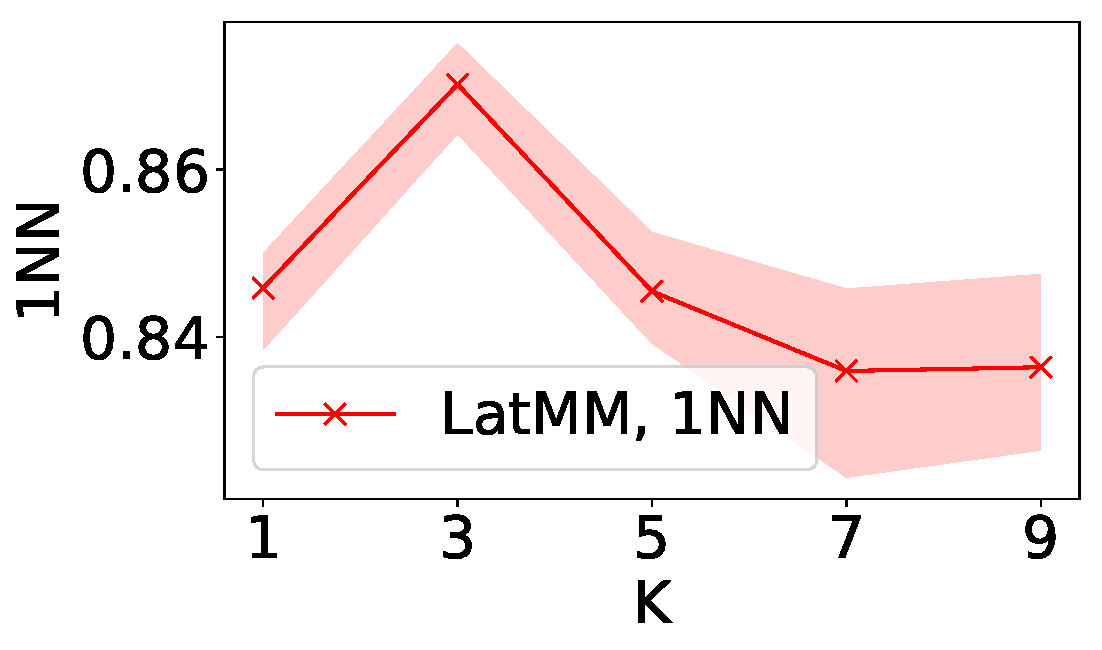
\includegraphics[width=1.\linewidth]{images/fashion-mnist/scores/std1EMGM-SM/EMGM-SM-1NN-K.pdf}
    % \caption{1NN score}
    % \label{fig-sm-1nn}
  \end{subfigure}
  \vspace{-0.35cm}
  \caption{IS, FID, MMD and 1NN of GenMM and LatMM for
    Fashion-MNIST dataset. GenMM and LatMM are trained on $60000$ images of Fashion-MNIST. The results are evaluated on $2000$ samples
    per simulation point ($1000$ samples generated by GenMM or LatMM
    for corresponding $K$, $1000$ samples from Fashion-MNIST). $5$
    experiments are carried out for each assessed score at each
    setting of $K$. Curve with marker denotes mean score and shaded
    area denotes the range of corresponding
    score.}\label{fig-scores-k-FashionMNIST}
  \vspace{0.2cm}
  % \vspace{10pt}
\end{figure*}
\subsection{Evaluation of Proposed Models}
In order to see if the proposed algorithms of GenMM and LatMM help to improve probability distribution modeling capacity, we assess our proposed algorithms with varying number of mixtures ($K$). Since our models are explicit models, the negative log likelihood (NLL) is used for comparison of our models. Apart from NLL, another four different metrics are used in assessment of models.
The metrics are Inception Score (IS) \cite{NIPS2016_6125,2018arXiv180101973B,2018arXiv180607755X}, Frechet
Inception Distance (FID) \cite{2017arXiv170608500H}, Maximum Mean
Discrepancy (MMD) \cite{2018arXiv180607755X} and two-sample test based 1-Nearest
Neighbor (1NN) score \cite{2016arXiv161006545L}. IS measures statistically if a given sample can be recognized by a classifier with high confidence. A high IS stands for high quality for generated samples. FID measures a divergence between two distributions under testing by assuming these two distribution are both Gaussian. We also use MMD with Gaussian kernel to test how dissimilar two distributions are.
Small values of FID and MMD mean that the mixture distribution model
is close to the underlying distribution of dataset. 1NN score measures
if two given distributions are empirically close by computing 1NN accuracy
on samples from two distributions under testing. The closer 1NN score is to $0.5$, the more likely 
two distributions under testing are the same. Therefore, a high IS is good, low FID and MMD scores, and 1NN score close to 0.5 are good. We use the evaluation
framework of \cite{2018arXiv180607755X} to compute these metrics scores, where
we train a ResNet on datasets MNIST and Fashion-MNIST, respectively, as the feature extractor for evaluation of the four performance metrics.

% \begin{table}%[htbp]
%   \centering
%   \caption{\textcolor{red}{Wrong Evaluation:NLL (nat/dim) of GenMM and LatMM on MNIST}}\label{tab-nll-genMM}
%   \begin{tabular}{l|r|rrrrr}
%     \toprule
%     \multirow{2}{*}{Dataset} &\multicolumn{5}{c}{K of GenMM} \\
%     \cline{2-6}
%     & 1 &   3 &   5 &   7 &   9 \\          
%     \hline                                                                                        
%     {Training} & 
%     4.208 &  4.167 &  4.015 &  4.043 &  4.067 \\                                 
%     \hline
%     Testing &  
%     4.197 &  4.165 &  4.025 &  4.053 &  4.075 \\    
%     \bottomrule
%   \end{tabular} 
%   \begin{tabular}{l|r|rrrrr}
%     \toprule
%     \multirow{2}{*}{Dataset}  & \multicolumn{5}{c}{K of LatMM} \\
%     \cline{2-6}
%     &   1 &   3 &   5 &   7 &   9 \\          
%     \hline                              
%     {Training} &
%     4.181 &  4.176 &  4.134 &  4.029 &  4.037 \\
%     \hline
%     {Testing}  &
%     4.195 &  4.178 &  4.144 &  4.042 &  4.049 \\                                \bottomrule
%   \end{tabular} 
% \end{table}

% \begin{table}%[htbp]
%   \centering
%   \caption{\textcolor{green}{Correction, Not positive result:NLL (nat/dim) of GenMM and LatMM on MNIST}}
%   \begin{tabular}{l|r|rrrrr}
%     \toprule
%     \multirow{2}{*}{Dataset} &\multicolumn{5}{c}{K of GenMM} \\
%     \cline{2-6}
%     & 1 &   3 &   5 &   7 &   9 \\          
%     \hline                                                                                        
%     {Training} & 
%     2.125 &  2.139 &  2.133 &  2.127 &  2.131 \\                                 
%     \hline
%     Testing &  
%     2.131 &  2.144 &  2.139 &  2.134 &  2.137 \\    
%     \bottomrule
%   \end{tabular} 
%   \begin{tabular}{l|r|rrrrr}
%     \toprule
%     \multirow{2}{*}{Dataset}  & \multicolumn{5}{c}{K of LatMM} \\
%     \cline{2-6}
%     &   1 &   3 &   5 &   7 &   9 \\          
%     \hline                              
%     {Training} &
%     2.127 &  2.134 &  2.133 &  2.114 &  2.138 \\
%     \hline
%     {Testing}  &
%     2.133 &  2.140 &  2.138 &  2.120 &  2.144 \\                                \bottomrule
%   \end{tabular} 
% \end{table}
% % \\on training:\\
% % \begin{tabular}{lrrrrr}                                                                                                                                       
%   \toprule                                                                                                                                                      
%   {} &   EMGM-1C &   EMGM-3C &   EMGM-5C &   EMGM-7C &   EMGM-9C \\                                                                                             
%   \midrule                                                                                                                                                      
%   0 &  4.208416 &  4.167086 &  4.015222 &  4.042882 &  4.066821 \\                                                                                              
%   1 &  4.208633 &  4.167396 &  4.015282 &  4.042878 &  4.066774 \\                                                                                              
%   2 &  4.208084 &  4.166920 &  4.015456 &  4.042807 &  4.066949 \\                                                                                              
%   3 &  4.208728 &  4.167286 &  4.015196 &  4.042803 &  4.066941 \\                                                                                              
%   4 &  4.208323 &  4.166983 &  4.015214 &  4.042674 &  4.066878 \\                                                                                              
%   \bottomrule                                                                                                                                                   
% \end{tabular}  

% \\testing\\

% \begin{tabular}{lrrrrr}                                                                                                                                       
%   \toprule                                                                                                                                                      
%   {} &   EMGM-1C &   EMGM-3C &   EMGM-5C &   EMGM-7C &   EMGM-9C \\                                                                                             
%   \midrule                                                                                                                                                      
%   0 &  4.196499 &  4.166211 &  4.025781 &  4.053625 &  4.075733 \\                                                                                              
%   1 &  4.198064 &  4.164900 &  4.025194 &  4.052824 &  4.075715 \\                                                                                              
%   2 &  4.196538 &  4.165242 &  4.024896 &  4.053364 &  4.074783 \\                                                                                              
%   3 &  4.198911 &  4.165181 &  4.025704 &  4.053324 &  4.076087 \\                                                                                              
%   4 &  4.198935 &  4.164621 &  4.026264 &  4.053708 &  4.075494 \\                                                                                              
%   \bottomrule                                                                                                                                                   
% \end{tabular}  

% \begin{table}[htbp]
%   \centering
%   \caption{NLL (nat/dim) of LatMM on MNIST}\label{tab-nll-latMM}
%   \begin{tabular}{l|r|rrrrr}
%     \toprule
%     \multirow{2}{*}{Dataset}  & \multicolumn{5}{c}{K of LatMM} \\
%     \cline{2-6}
%     &   1 &   3 &   5 &   7 &   9 \\          
%     \hline                              
%     {Training} &
%     4.181 &  4.176 &  4.134 &  4.029 &  4.037 \\
%     \hline
%     {Testing}  &
%     4.195 &  4.178 &  4.144 &  4.042 &  4.049 \\                                \bottomrule
%   \end{tabular}                                                                                    \end{table}

% training \\
% \begin{tabular}{lrrrrr}                                                                                                                                       
%   \toprule                                                                                                                                                      
%   {} &   EMGM-1S &   EMGM-3S &   EMGM-5S &   EMGM-7S &   EMGM-9S \\                                                                                             
%   \midrule                                                                                                                                                      
%   0 &  4.180553 &  4.176250 &  4.134201 &  4.028757 &  4.037176 \\                                                                                              
%   1 &  4.181187 &  4.176145 &  4.134370 &  4.028634 &  4.036834 \\                                                                                              
%   2 &  4.181523 &  4.176267 &  4.134102 &  4.028518 &  4.036781 \\                                                                                              
%   3 &  4.180647 &  4.176359 &  4.134188 &  4.028753 &  4.036891 \\                                                                                              
%   4 &  4.181394 &  4.176374 &  4.134405 &  4.028574 &  4.036821 \\                                                                                              
%   \bottomrule                                                                                                                                                   
% \end{tabular} 

% testing \\
% \begin{tabular}{lrrrrr}                                                                                                                                       
%   \toprule                                                                                                                                                      
%   {} &   EMGM-1S &   EMGM-3S &   EMGM-5S &   EMGM-7S &   EMGM-9S \\                                                                                             
%   \midrule                                                                                                                                                      
%   0 &  4.194728 &  4.178272 &  4.143965 &  4.041466 &  4.049319 \\                                                                                              
%   1 &  4.194917 &  4.178052 &  4.143046 &  4.041250 &  4.048735 \\                                                                                              
%   2 &  4.194268 &  4.178865 &  4.143759 &  4.041944 &  4.048040 \\                                                                                              
%   3 &  4.195079 &  4.177494 &  4.143818 &  4.041399 &  4.049067 \\                                                                                              
%   4 &  4.194052 &  4.179352 &  4.143538 &  4.041786 &  4.048846 \\                                                                                              
%   \bottomrule                                                                                                                                                   
% \end{tabular}   


% \begin{table}
%   \centering
%   \caption{The lowest NLL value of LatMM for curves in \autoref{fig:latmm-nll} (nat/pixel).}
%   \label{tab:lowestNLLlatMM}
%   \begin{tabular}{l|c|c|c|c}\toprule
%     \toprule
%     {Dataset} &  K=1 &  K=3 &  K=5 &  K=7 \\
%     \midrule
%     MNIST &   1.9450 &   1.9384 &    1.9379 &    1.9341 \\ \midrule
%     Fashion-MNIST &   2.6091 &   2.4405 &   2.4385 &   2.4157 \\
%     \bottomrule
%   \end{tabular}
% \end{table}


\begin{table}
  \caption{The lowest NLL value of GenMM for curves in \autoref{fig:genmm-nll} (nat/pixel).}
  \label{tab:lowestNLLgenMM}
  % \centering
  \begin{tabular}{l|c|c|c|c}
    \toprule
    {Dataset} & K=1 &  K=3 &  K=5 &  K=7 \\                                         
    \midrule                                                                                          MNIST &     1.8929 &    1.8797 &    1.8719 &    1.8579 \\
    FashionMNIST &   2.3571 &   2.3429 &   2.3353 &   2.3323 \\ 
  \end{tabular} 
\end{table}
The NLL curves of GenMM and LatMM models during model training phase are shown in \autoref{fig:genmm-nll} and \autoref{fig:latmm-nll}, respectively. Subsets of MNIST and Fashion-MNIST are used to train our mixture models in order to assess their performance w.r.t. NLL when different number of mixture components $K$ is used. All the curves in \autoref{fig:genmm-nll} and \autoref{fig:latmm-nll} show that NLL decreases as training epoch number increases in general. There is fluctuation of these decreasing NLL curves due to: (a) the iteration of E-step and M-step of EM, and (b) the use of batch-size gradient in optimization at M-step. In each figure of \autoref{fig:genmm-nll} and \autoref{fig:latmm-nll}, NLL curve corresponding to larger total number of mixture components, $K$, reaches smaller NLL value after traning for same number of epochs. The results are consistent since as $K$ increases, both GenMM and LatMM have smaller NLL. These results confirm our hypothesis that mixture models fit real data better. The lowest NLL values of curves in \autoref{fig:genmm-nll} in training GenMM models are reported in \autoref{tab:lowestNLLgenMM}.

\begin{figure*}[!ht]
  \captionsetup[subfigure]{justification=centering}
  \centering
  \begin{subfigure}[b]{0.24\textwidth}
    \centering
    % 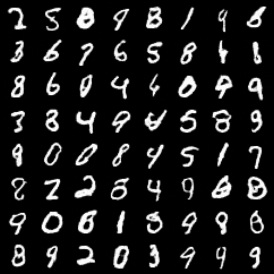
\includegraphics[width=1\linewidth]{images/mnist/samples/gen_c12_std08.png}
    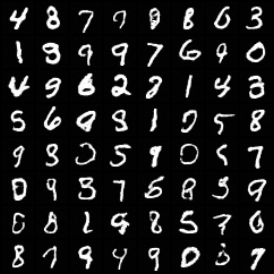
\includegraphics[width=1\linewidth]{images/mnist/samples/genMNIST_GenMM_K7_std089.png}
    \caption{Generated Samples. (GenMM, K=7)}
  \end{subfigure}
  % \begin{subfigure}[b]{0.19\textwidth}
  %   \centering
  %   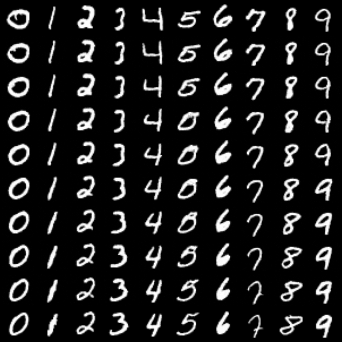
\includegraphics[width=1\linewidth]{images/mnist/interpolation/interpo_c12_mnist_std07.png}
  %   \caption{Interpolation. (GenMM, K=12)}\label{fig-interpo}
  % \end{subfigure}
  \centering
  \begin{subfigure}[b]{0.24\textwidth}
    \centering
    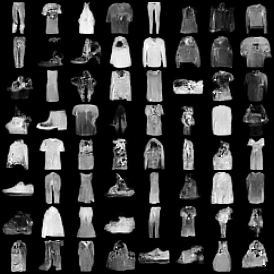
\includegraphics[width=1\linewidth]{images/fashion-mnist/samples/gene_c3_std1_samples.png}
    \caption{Generated samples. (GenMM, K=3)}
  \end{subfigure}
  \begin{subfigure}[b]{0.24\textwidth}
    \centering
    % 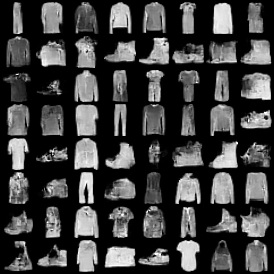
\includegraphics[width=1\linewidth]{images/fashion-mnist/samples/gen_s5_std1.png}
    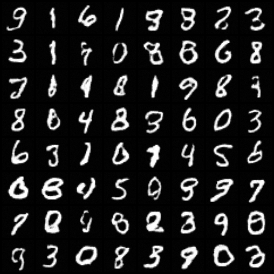
\includegraphics[width=1\linewidth]{images/mnist/samples/gen_LatMM_K3_std088.png}
    \caption{Generated samples. (LatMM, K=3)}
  \end{subfigure}
  \begin{subfigure}[b]{0.24\textwidth}
    \centering
    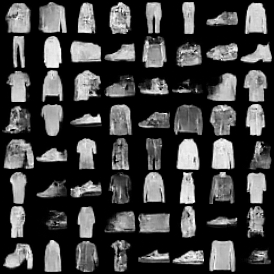
\includegraphics[width=1\linewidth]{images/fashion-mnist/samples/gen_s7_std1.png}
    \caption{Generated samples. (LatMM, K=7)}
  \end{subfigure}
  % \begin{subfigure}[b]{0.23\textwidth}
  %   \centering
  %   \includegraphics[width=1\linewidth]{images/fashion-mnist/samples/gene_c7_std1_samples.png}
  %   \caption{Generated samples. (EMGM-NM, K=7)}
  % \end{subfigure}
  \vspace{-0.3cm}
  \caption{Generated samples by GenMM and LatMM for MNIST and Fashion-MNIST datasets.}\label{fig-demo-samples}
  % \vspace{0.5cm}
\end{figure*}
% \begin{figure}
%   \centering
%   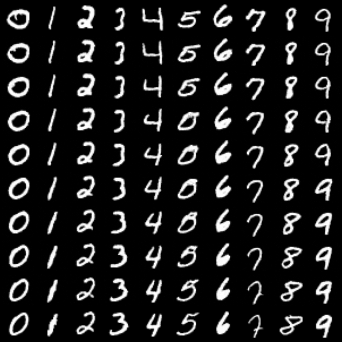
\includegraphics[width=.6\linewidth]{images/mnist/interpolation/interpo_c12_mnist_std07.png}
%   \caption{Interpolation in latent space to generate samples. We use GenMM with K=12.}
%   \vspace{0.5cm}
% \end{figure}

\begin{figure*}[!ht]
  \centering
  \captionsetup[subfigure]{justification=centering}
  \begin{subfigure}[b]{0.3\textwidth}
    \centering
    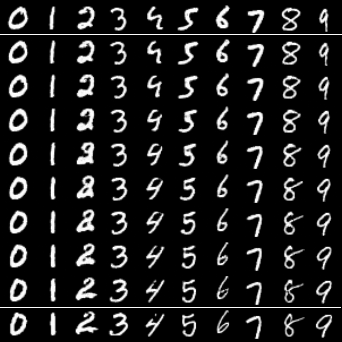
\includegraphics[width=1\linewidth]{images/mnist/interpolation/interpoMNIST_homo_GenMM_K7_map_grid.png}
    \caption{Interpolation by GenMM, K=7. Identity of $\bm{g}_k$ is chosen by $\argmax_{k}\; \gamma_k$.}\label{fig-interpo-genmm1}
  \end{subfigure}
  \hspace{10pt}
  \begin{subfigure}[b]{0.3\textwidth}
    \centering
    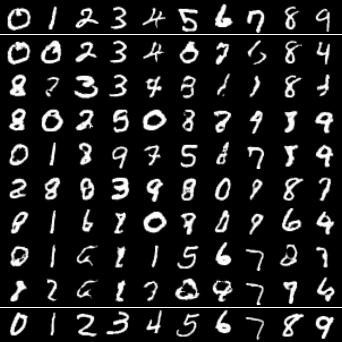
\includegraphics[width=1\linewidth]{images/mnist/interpolation/interpoMNIST_GenMM_K7_random_grid.png}
    \caption{Interpolation by GenMM, K=7. Identity of $\bm{g}_k$ is randomly chosen.}\label{fig-interpo-genmm2}
  \end{subfigure}
  \hspace{10pt}
  \begin{subfigure}[b]{0.3\textwidth}
    \centering
    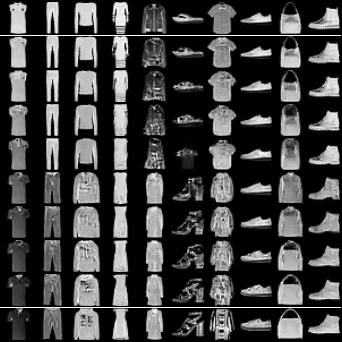
\includegraphics[width=1\linewidth]{images/fashion-mnist/interpolation/interpoFashion_homo_GenMM_K9_map_grid.png}
    \caption{Interpolation by GenMM, K=9. Identity of $\bm{g}_k$ is chosen by $\argmax_{k}\; \gamma_k$.}\label{fig-interpo-genmm3}
  \end{subfigure}
  % \caption{Interpolation in latent space to generate samples . GenMM}\label{fig-interpo}
  \vspace{0.22cm}
  % \label{fig-app-interpolation}
  % \vspace{0.2cm}
  % \end{figure*}
  % \begin{figure*}[!ht]
  \centering
  \captionsetup[subfigure]{justification=centering}
  \begin{subfigure}[b]{0.3\textwidth}
    \centering
    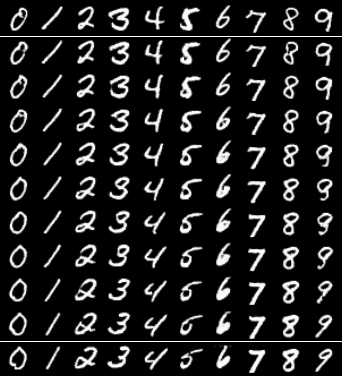
\includegraphics[width=1\linewidth]{images/mnist/interpolation/LatMMK9interpo_sample_grid.png}
    \caption{Interpolation by LatMM, K=9.}\label{fig-interpo-latmm1}
  \end{subfigure}
  \hspace{10pt}
  \begin{subfigure}[b]{0.3\textwidth}
    \centering
    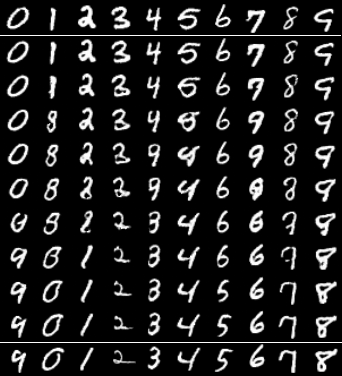
\includegraphics[width=1\linewidth]{images/mnist/interpolation/interpoMNIST_heter_LatMM_K9_sample_grid.png}
    \caption{Interpolation by LatMM, K=9.}\label{fig-interpo-latmm2}
  \end{subfigure}
  \hspace{10pt}
  \begin{subfigure}[b]{0.3\textwidth}
    \centering
    \includegraphics[width=1\linewidth]{images/fashion-mnist/interpolation/interpoFashion_heter_LatMM_K9_grid.png}
    \caption{Interpolation by LatMM, K=9.}\label{fig-interpo-latmm3}
  \end{subfigure}\vspace{-0.5cm}
  \caption{Interpolation in latent space to generate samples . First
    and last rows are real samples from MNIST. For each row, images
    are generated by interpolating latent variables of empirical
    images in first and last rows.}\label{fig-interpo}
  \vspace{0.2cm}
  \label{fig-app-interpolation}
  % \vspace{0.2cm}
\end{figure*}


As for the scores of IS, FID, MMD, and 1NN, we increase $K$ for the proposed models and check
how the four metrics vary. We do several trials of evaluation and
report the results. The results are shown in
\autoref{fig-scores-k} for MNIST datset and
\autoref{fig-scores-k-FashionMNIST} for Fashio-MNIST dataset. Let us
first address the results in \autoref{fig-scores-k}. It can be
observed that IS increases with number of mixtures $K$. The IS
improvement shows a saturation and decreasing trend for GenMM when
$K=9$. The FID, MMD and 1NN scores show a decreasing trend with
increase in $K$. Their trends also saturate with increase in $K$. The
trends obey a statistical knowledge that performance improves with
increase in the model complexity, and then deteriorates if the model
complexity continues to increase. As that in \autoref{fig-scores-k}, similar trends are also observed in \autoref{fig-scores-k-FashionMNIST}. In some cases, performance for $K=3$ is poorer than $K=1$. We assume that the random initialization of parameters in mixture models has a high influence in this regard. 
Considering the trends in all the scores for both the figures, we can conclude that GenMM and LatMM can model the underlying distributions of data and the mixture models are good.
% Therefore, if we want to model a datset's distribution using our proposed GenMM or LatMM models with large modeling capacity, it can be done by using large number of mixture components. When increasing $K$ from $1$ to $3$, $5$, $7$, the comparison between GenMM's NLL curves in \autoref{fig:genmm-nll} and LatMM's NLL curves in \autoref{fig:latmm-nll} shows that the NLL curve gap (the gain) of GenMM is larger than that of LatMM. This is consistent with our discussion about the model complexity of GenMM and LatMM in \autoref{sec:complexity}, i.e. GenMM is more complex than LatMM and we can expect GenMM has better modeling capacity than LatMM when generator networks are similarly complex. One exception happens between curve of $K=1$ and that of $K=3$ for LatMM in \autoref{fig-latmm-fsh-nll-curve}. This could be due to totally random initialization of all neural networks parameters.

% We also list the lowest NLL value observed in each curve of \autoref{fig-genmm-mnist-nll-curve}, \autoref{fig-genmm-fsh-nll-curve}, \autoref{fig-latmm-mnist-nll-curve}, and \autoref{fig-latmm-mnist-nll-curve}. They are shown in \autoref{tab:lowestNLLgenMM} and \autoref{tab:lowestNLLlatMM}. As expected, the lowest NLL value decreases as $K$ increases for both GenMM and LatMM trained on two datasets. Again, the NLL value dropping gap for GenMM is larger than that for LatMM in general sense.

% We report NLL versus number of mixture omponents ($K$). To
% avoid numerical computation problem of log-sum for high-dimension
% signal, the $\log{P_k(\bm{x})}$ is scaled 
% \footnote{Direct computation of log-likelihood
% $\log{\sum_{k=1}^{K}\;\pi_k P_k(\bm{x})}$ for high dimensional
% signal $\bm{x}$ is numerically problematic. Then the scaled NLL is
% actually reported as $\log{\sum_{k=1}^{K}\pi_k
% \left(P_k(\bm{x})\right)^{1/\mathrm{dim}(\bm{x})}}$.} by dimension of $\bm{x}$,
% \emph{i.e.} $\mathrm{dim}(\bm{x})$, and we report NLL via unit of nat
% per dimension (nat/dim).




% The tables 1 and 2 show the NLL where we use MNIST dataset. The training dataset of MNIST is used for learning the model parameters. The testing dataset of MNIST is used to verify how the trained models fit for unseen test dataset. We observe from the tables that the NLL decreases with increase in $K$ and then shows a timid upward trend. This NLL behaviour is consistent with a usual statistical knowledge that performance improves with increase in model complexity and then deteriorates if model complexity continues to increase. Also, we observe that NLL for testing dataset is close to the NLL for training dataset. This shows that our proposed models and developments of EM algorithms are able to address generalization property.

% Using the trained models for the first experiment, we report four more
% scores to show performance versus model complexity. The IS, FID, MMD
% and INN scores are shown in \autoref{fig-scores-k}. For this figure,
% we did a random selection of 1000 data samples from training dataset;
% this is true data. Then we generated 1000 data samples using trained
% models. We used 1000 (true) real data and 1000 generated data to
% compute the scores. The scores are computed for several trials. In the
% \autoref{fig-scores-k}, a solid line is the average of trials and the shaded region shows the range of scores across the average score.       


\subsection{Sample Generating and Interpolation}

\begin{table*}
  \caption{Test Accuracy Table of GenMM for Classification Task}\label{tab:acc-classification}
  % \centering
  % \subcaption{Accuracy Table of GenMM on Test Data}
  % \centering  
  \begin{tabular}{l|c|c|c|c|c|c|c} \toprule
    {Dataset} &  K=1 &  K=2 &  K=3 &  K=4 & K=10 & K=20 & State Of Art \\ \midrule
    Letter & 0.9459 &  0.9513 & 0.9578  & 0.9581 & 0.9657 & \textbf{0.9674} & {0.9582} \cite{tang2016extreme} \\ \midrule
    Satimage & 0.8900 & 0.8975 & 0.9045 & 0.9085 & 0.9105 & \textbf{0.9160} & 0.9090 \cite{jiang2013k-svd}   \\ \midrule
    Norb & 0.9184 & 0.9257 & 0.9406 & 0.9459 & 0.9538 & \textbf{0.9542} & 0.8920 \cite{pmlr-v5-salakhutdinov09a}  \\
    % \bottomrule
  \end{tabular}
  % \centering
  % \subcaption{Accuracy Table of LatMM}
  % \centering  
  % \begin{tabular}{l|c|c|c|c|c}
  %   \toprule
  %   {Dataset} &  K=1 &  K=2 &  K=3 &  K=4 &  State of Art \\
  %   \midrule
  %   Letter & 0.9453 &  0.9421 &  0.9462 &   0.9469 &  0.9582 \cite{tang2016extreme} \\ \midrule
  %   Satimage & 0.8855 & 0.8895 & 0.8730 & 0.8895 & 0.9090 \cite{jiang2013k-svd} \\ \midrule
  %   Norb & 0.9315 & 0.9221 & 0.9151 & 0.9274 & 0.8920 \cite{pmlr-v5-salakhutdinov09a} \\
  %   \bottomrule                                                                  
  % \end{tabular}                                                                
\end{table*}
\begin{figure*}[!ht]
  \captionsetup[subfigure]{justification=centering}
  \centering
  \begin{subfigure}{.33\textwidth}
    \centering
    \includegraphics[width=1\linewidth]{images/supply/train_curves/letter_1.pdf}
    \vspace{-0.8cm}
    \caption{K=1}
    % \label{fig-nm-isk}
  \end{subfigure}
  \begin{subfigure}{.33\textwidth}
    \centering
    \includegraphics[width=1\linewidth]{images/supply/train_curves/letter_2.pdf}
    \vspace{-0.8cm}
    \caption{K=2}
    % \caption{FID score}
    % \label{fig-nm-fidk}
  \end{subfigure}
  \centering
  \begin{subfigure}{.33\textwidth}
    \centering
    \includegraphics[width=1\linewidth]{images/supply/train_curves/letter_3.pdf}
    \vspace{-0.8cm}
    \caption{K=3}
    % \caption{MMD score}
    % \label{fig-nm-mmdk}
  \end{subfigure}
  \centering
  \begin{subfigure}{0.33\textwidth}
    \centering
    \includegraphics[width=1\linewidth]{images/supply/train_curves/letter_4.pdf}
    \vspace{-0.8cm}
    \caption{K=4}
    % \caption{1NN score}
    % \label{fig-nm-1nnk}
  \end{subfigure}
  \centering
  \begin{subfigure}{.33\textwidth}
    \centering
    \includegraphics[width=1\linewidth]{images/supply/train_curves/letter_10.pdf}
    \vspace{-0.8cm}
    \caption{K=10}
    % \caption{IS score}
    % \label{fig-sm-is}
  \end{subfigure}
  \centering
  \begin{subfigure}{.33\textwidth}
    \centering
    \includegraphics[width=1\linewidth]{images/supply/train_curves/letter_20.pdf}
    \vspace{-0.8cm}
    \caption{K=20}
    % \caption{FID score}
    % \label{fig-sm-fid}
  \end{subfigure}
  \vspace{-0.3cm}
  \caption{Train and Test Accuracy Curves versus Epochs on Dataset Letter.}
  \label{fig:class-letter}
  \vspace{0.2cm}
\end{figure*}




Next we show generated samples from the proposed models trained with MNIST and Fashion-MNIST in \autoref{fig-demo-samples}. In the figure, we show generated samples from GenMM and LatMM for MNIST and Fashion-MNIST datasets. We use different value of $K$ to generate images. It can be observed that LatMM is able to produce good quality image samples as GenMM. While we argue that LatMM has a lower level of complexity than GenMM, it is seen that LatMM works good in practice.    

In the second experiment, we explore power of invertibility for interpolation in the latent domain. We use samples from MNIST and Fashion-MNIST datasets for this `interpolation' experiment. In \autoref{fig-interpo}, we have six subfigures. For each subfigure, the first row and the last row are comprised of the real (true) data samples from MNIST and Fashion-MNIST dataset. In each column, we find latent codes corresponding to the real samples of the first row and the last row, $\bm{z}_1, \bm{z}_2$. This is possible as the neural networks are invertible. Then, we perform a convex combination of the two latent codes as $\alpha \bm{z}_1 + (1- \alpha)\bm{z}_2$, where $0 < \alpha <1$. The latent code produced by the convex combination is used to generate a new sample using the trained models. All other rows except the first and the last rows of the figure are the generated samples by varying $\alpha$. In \autoref{fig-interpo}, we observe the change visually from the first row to last row - how the first row slowly changes to the last row. We use GenMM for \autoref{fig-interpo-genmm1}, \autoref{fig-interpo-genmm2}, \autoref{fig-interpo-genmm3}, and LatMM for \autoref{fig-interpo-latmm1}, \autoref{fig-interpo-latmm2}, \autoref{fig-interpo-latmm3}. Interpolation experiment for LatMM is easier than GenMM. GenMM has a set of neural network generators $\{ \bm{g}_k(\bm{z}) \}_{k=1}^K$ and a fixed Gaussian distribution for latent variable $\bm{z}$. We compute $\gamma_k$ for a real image $\bm{x}$, and then find the latent code $\bm{z}$ of $\bm{x}$ using $\bm{g}_{k^{*}}^{-1}(\bm{x})=\bm{f}_{k^{*}}(\bm{x})$, where $k^{*} = \arg \max_{k} \gamma_k$. For two real images (one image is in the first row and the second image in the last row), we find the corresponding latent codes, compute their convex combination as interpolation, and then pass the computed latent code through a generator $\bm{g}_k(\bm{z})$ to produce a generated sample $\bm{x}$. Identity of the generator of GenMM is chosen as $k^{*}$ corresponding to the image of the first row if $\alpha < 0.5$, or to the image of the last row if $\alpha \geq 0.5$.

\begin{figure*}[!ht]
  \captionsetup[subfigure]{justification=centering}
  \centering
  \begin{subfigure}{.33\textwidth}
    \centering
    \includegraphics[width=1\linewidth]{images/supply/train_curves/norb_1.pdf}
    \vspace{-0.8cm}
    \caption{K=1}
    % \caption{IS score}
    % \label{fig-nm-isk}
  \end{subfigure}
  \vspace{-2pt}
  \begin{subfigure}{.33\textwidth}
    \centering
    \includegraphics[width=1\linewidth]{images/supply/train_curves/norb_2.pdf}
    \vspace{-0.8cm}
    \caption{K=2}
    % \caption{FID score}
    % \label{fig-nm-fidk}
  \end{subfigure}
  \centering
  \begin{subfigure}{.33\textwidth}
    \centering
    \includegraphics[width=1\linewidth]{images/supply/train_curves/norb_3.pdf}
    \vspace{-0.8cm}
    \caption{K=3}
    % \caption{MMD score}
    % \label{fig-nm-mmdk}
  \end{subfigure}
  \centering
  \begin{subfigure}{0.33\textwidth}
    \centering
    \includegraphics[width=1\linewidth]{images/supply/train_curves/norb_4.pdf}
    \vspace{-0.8cm}
    \caption{K=4}
    % \caption{1NN score}
    % \label{fig-nm-1nnk}
  \end{subfigure}
  \centering
  \begin{subfigure}{.33\textwidth}
    \centering
    \includegraphics[width=1\linewidth]{images/supply/train_curves/norb_10.pdf}
    \vspace{-0.8cm}
    \caption{K=10}
    % \caption{IS score}
    % \label{fig-sm-is}
  \end{subfigure}
  \centering
  \begin{subfigure}{.33\textwidth}
    \centering
    \includegraphics[width=1\linewidth]{images/supply/train_curves/norb_20.pdf}
    \vspace{-0.8cm}
    \caption{K=20}
    % \caption{FID score}
    % \label{fig-sm-fid}
  \end{subfigure}
  \vspace{-0.3cm}
  \caption{Train and Test Accuracy Curves versus Epochs on Dataset Norb}
  \label{fig:class-norb}
\end{figure*}


The second experiment on interpolation shows interesting result for
modeling multi-modal data. The distribution of ten digits together in
MNIST dataset is expected to be multi-modal. The aspect of multi-modal
distribution is addressed using the experimental result shown in
\autoref{fig-interpo-genmm2}. We use similar experimental steps
as that in \autoref{fig-interpo-genmm1} but with modifications. It
is evident that the generated digit images do not correspond well to
the real images of the first row and the last row. For example, in the
first column of \autoref{fig-interpo-genmm2}, we observe
presence of digits two and eight, while we expect that the
column should be comprised of only images of digit zero. Natural
question is why interpolation leads to generation of digits that are
unexpected. The answer lies in the procedure of performing our
experiment. The key difference for this experiment compared to the
experiment in \autoref{fig-interpo-genmm1} is that a sample is
produced by a randomly selected generator $\bm{g}_k(\bm{z})$ from $K$
possible choices. We compute interpolated latent code using the same
procedure as that in \autoref{fig-interpo-genmm1}, but use the generator where its identity $k$ is randomly sampled from the prior $\bm{\pi}$ directly. The generated images in this interpolation experiment reveals a clue that each generator models a subset of the whole training dataset. We can qualitatively argue that use of multiple generators helps for modeling the multi-modal distribution.  

\subsection{Application to Classification Task}
\begin{figure*}[!ht]
  \captionsetup[subfigure]{justification=centering}
  \centering
  \begin{subfigure}{.33\textwidth}
    \centering
    \includegraphics[width=1\linewidth]{images/supply/train_curves/satimage_1.pdf}
    \vspace{-0.8cm}
    \caption{K=1}
    % \caption{IS score}
    % \label{fig-nm-isk}
  \end{subfigure}
  \vspace{-2pt}
  \begin{subfigure}{.33\textwidth}
    \centering
    \includegraphics[width=1\linewidth]{images/supply/train_curves/satimage_2.pdf}
    \vspace{-0.8cm}
    \caption{K=2}
    % \caption{FID score}
    % \label{fig-nm-fidk}
  \end{subfigure}
  \centering
  \begin{subfigure}{.33\textwidth}
    \centering
    \includegraphics[width=1\linewidth]{images/supply/train_curves/satimage_3.pdf}
    \vspace{-0.8cm}
    \caption{K=3}
    % \caption{MMD score}
    % \label{fig-nm-mmdk}
  \end{subfigure}
  \centering
  \begin{subfigure}{0.33\textwidth}
    \centering
    \includegraphics[width=1\linewidth]{images/supply/train_curves/satimage_4.pdf}
    \vspace{-0.8cm}
    \caption{K=4}
    % \caption{1NN score}
    % \label{fig-nm-1nnk}
  \end{subfigure}
  \centering
  \begin{subfigure}{.33\textwidth}
    \centering
    \includegraphics[width=1\linewidth]{images/supply/train_curves/satimage_10.pdf}
    \vspace{-0.8cm}
    \caption{K=10}
    % \caption{IS score}
    % \label{fig-sm-is}
  \end{subfigure}
  \centering
  \begin{subfigure}{.33\textwidth}
    \centering
    \includegraphics[width=1\linewidth]{images/supply/train_curves/satimage_20.pdf}
    \vspace{-0.8cm}
    \caption{K=20}
    % \caption{FID score}
    % \label{fig-sm-fid}
  \end{subfigure}
  \vspace{-0.3cm}
  \caption{Train and Test Accuracy Curves versus Epochs on Dataset Satimage.}
  \vspace{0.3cm}
  \label{fig:class-satimage}
\end{figure*}
In this subsection, we apply our proposed mixture models to classification tasks using the maximum likelihood criterion. We compare classification performance with the state-of-art results. The state-of-art results are produced by discriminative learning approaches. The major advantage of maximum likelihood based classification is that any new class can be accommodated on-the-fly. On the contrary a discriminative learning approach requires retraining whenever new classes appear. 

For a given dataset with $Y$ classes, we divide the dataset by sample labels and each subset has the same label $y$. Then we train one GenMM model per class of data, i.e. $p(\bm{x};\bm{\Phi}_{y})$ is trained with the $y$-th class's data. After we have all $p(\bm{x};\bm{\Phi}_y)$, $\forall y = 1, 2, \cdots, Y$ trained, a new sample $\bm{x}$ is predicted by $\argmax_{y} p(\bm{x};\bm{\Phi}_y)$.

The maximum likelihood based classification experiment as described above is carried out in three different datasets: Letter, Satimage, and Norb. For each dataset, we train our models for $300$ epoches on the training data of the corresponding dataset, and the test accuracy is reported in \autoref{tab:acc-classification}. The state-of-art accuracy of each dataset in literature is also listed in this table for comparison. For each dataset, we increase the total number of mixture components $K$ and the neural network generators have the same structure. The table shows that the classification accuracy on each dataset is increased as we increase the number of generators in GenMM. When $K$ is $10$ or $20$, maximum likelihood based classification by GenMM outperforms the state-of-art accuracy. The state-of-art accuracy results are obtained by using discriminative learning approaches. For dataset Norb, more significant performance gain is observed. Our classification accuracy is boosted from $0.9184$ to $0.9542$ when $K$ is increased from $1$ to $20$ and a large improvement margin is obtained over reference accuracy. We also test LatMM on classification task, but its accuracy is more or less around the accuracy of GenMM with $K=1$. Note that LatMM is a relatively low-complexity model than GenMM. 
% The latent source mixture strategy of LatMM is not as powerful as GenMM to model multi-modal data.

\autoref{fig:class-letter} \autoref{fig:class-satimage} and \autoref{fig:class-norb} show the train and test accuracy changing along with the training epoch on dataset Letter and Satimage, respectively. For each dataset, the accuracy curves versus epoch trained with GenMM at different value of $K$ are shown. In these sets of figures, all accuracy curves climbs and flattens around some value, as training epoch increases. Train accuracy is either coincident with, or above test accuracy curve at different training phases. For each set of figures on a given dataset, the gap between train and test curve is smaller as a larger number of mixture components is used. As $K$ increases, test curve flattens at a larger accuracy value. This again speaks for validation of our proposed models and also the advantage of using our mixture models for practical tasks.

\section{Conclusion}
We conclude that the principal of expectation maximization can be used for neural network based probability distribution modeling. Our approach leads to explicit distribution modeling and the experimental results show an important aspect that the normal statistical behaviour of modeling performance versus model complexity remains valid. The proposed models are able to generate images which have good visual quality. This is also supported by several metric scores. Practical applications of our models for classification tasks are also carried out. The results confirm that our approach is good for modeling multi-modal distributions.
Further extensions using variational inference for learning
parameters of mixture models will be studied in the future.


%%% Local Variables:
%%% mode: latex
%%% TeX-master: "../../main"
%%% End:
